 
%%%%%%%%%%%%%%%%%%%%%%%%%%%%%%%%%%%%%%%%%%%%%%
%%                                          %%
%%         DOCUMENT FROM TEMPLATE           %%
%%                                          %%
%%%%%%%%%%%%%%%%%%%%%%%%%%%%%%%%%%%%%%%%%%%%%%
\documentclass[journal]{IEEEtran}
%\IEEEoverridecommandlockouts 
%\overrideIEEEmargins          

\usepackage{amsmath,amssymb,amsfonts}
\usepackage{graphicx}
\usepackage{textcomp}

%%%%%%%%%%%%%%%%%%%%%%%%%%%%%%%%%%%%%%%%%%%%%%
%%                                          %%
%%           ADDITIONAL PACKAGES            %%
%%                                          %%
%%%%%%%%%%%%%%%%%%%%%%%%%%%%%%%%%%%%%%%%%%%%%%
\usepackage{amsthm}
\usepackage{xcolor}
\usepackage[figuresright]{rotating}

\usepackage{graphicx}
\graphicspath{{/}{fig/}}

\usepackage{array}
\usepackage{textcomp}
\usepackage{xcolor}
\usepackage{multirow}
\usepackage{booktabs}
\usepackage{enumitem}

\usepackage{mathtools}
\usepackage{breqn}
\usepackage{float}

\usepackage{caption}
% \captionsetup{format=hang}
\captionsetup{font=small}
\usepackage{subcaption}%for subfigures as well

\usepackage{mathtools}
\usepackage{float}
\usepackage{hyperref}

\usepackage{pgfplots}
\pgfplotsset{compat=1.7}
\usepgfplotslibrary{groupplots}

\usepackage{multirow,tabularx}
\usepackage{flushend}

%%%%%%%%%%%%%%%%%%%%%%%%%%%%%%%%%%%%%%%%%%%%%%
%%                                          %%
%%              NEW COMMANDS                %%
%%                                          %%
%%%%%%%%%%%%%%%%%%%%%%%%%%%%%%%%%%%%%%%%%%%%%%

\newcommand{\np}{\vspace{7mm}}
\newcommand{\red}{\textcolor{red}}
\newcommand{\blue}{\textcolor{blue}}


\newcommand*\circled[1]{\tikz[baseline=(char.base)]{
            \node[shape=circle,draw,inner sep=2pt] (char) {#1};}}
    

\newcommand*{\defeq}
    {\mathrel{
        \vcenter{
            \baselineskip0.5ex \lineskiplimit0pt
            \hbox{\scriptsize.}\hbox{\scriptsize.}}}%
    =}

\DeclareMathOperator*{\argmin}{argmin}

\newtheorem{lemma}{Lemma}
\newtheorem{theorem}{Theorem}
\newtheorem{problem}{Problem}
\newtheorem{definition}{Definition}
\newtheorem{assumption}{Assumption}
\newtheorem{proposition}{Proposition}

\newlength\figureheight
\newlength\figurewidth
\setlength\figureheight{0.23\textwidth}
\setlength\figurewidth{0.24\textwidth}

\newcommand{\donemark}{\textcolor{donegreen}{\underline{\textbf{DONE \ding{51}}}}}

%%%%%%%%%%%%%%%%%%%%%%%%%%%%%%%%%%%%%%%%%%%%%%
%%                                          %%
%%            TITLE AND AUTHORS             %%
%%                                          %%
%%%%%%%%%%%%%%%%%%%%%%%%%%%%%%%%%%%%%%%%%%%%%%
\title{\LARGE \bf
    Towards Closing the Sim-to-Real Gap in \\ Collaborative Multi-Robot Deep Reinforcement Learning
}

\author{
    \IEEEauthorblockN{
        Wenshuai Zhao\textsuperscript{1},
        Jorge Pe\~{n}a Queralta\textsuperscript{1},
        Li Qingqing\textsuperscript{1},
        Tomi Westerlund\textsuperscript{1}
    }\\[6pt]
    \IEEEauthorblockA{
        \textsuperscript{1} \href{https://tiers.utu.fi}{Turku Intelligent Embedded and Robotic Systems Lab, University of Turku, Finland} \\
        Emails: \textsuperscript{1}\{wezhao, jopequ, qingqli, tovewe\}@utu.fi
    }
}

%%%%%%%%%%%%%%%%%%%%%%%%%%%%%%%%%%%%%%%%%%%%%%
%%                                          %%
%%             BEGIN DOCUMENT               %%
%%                                          %%
%%%%%%%%%%%%%%%%%%%%%%%%%%%%%%%%%%%%%%%%%%%%%%
\begin{document}


%%%%%%%%%%%%%%%%%%%%%%%%%%%%%%%%%%%%%%%%%%%%%%
%%                                          %%
%%              PAPER CONTENT               %%
%%                                          %%
%%%%%%%%%%%%%%%%%%%%%%%%%%%%%%%%%%%%%%%%%%%%%%
\maketitle

\input{sections/00_Abstract.tex}

\section{Introduction}

Reinforcement learning (RL) algorithms for robotics and cyber-physical systems have seen an increasing adoption across multiple domains over the past decade~\cite{arulkumaran2017brief, nguyen2020deep}. Deep reinforcement learning (DRL) enables agents to be trained in realistic environments without the need for large amounts of data to be gathered and labeled a priori. Specifically, reinforcement learning has enjoyed significant success in robotic control tasks involving manipulation~\cite{mnih2016asynchronous, rajeswaran2017learning, matas2018sim}. Motivated by the way humans and animals learn, DRL algorithms work on a \textit{trial and error} basis, where an agent interacts with its environment and receives a reward based on its performance. When complex agents or environments are involved, the learning process can be relatively slow. This has motivated the design and development of multi-agent DRL algorithms. In this paper, we are interested in exploring some of the challenges remaining in multi-robot collaborative DRL.

\begin{figure}
    \centering
    \includegraphics[width=0.48\textwidth]{fig/concept_v3.pdf}
    \caption{Conceptual view of the proposed scenario, where multiple robotic agents are collaboratively learning the same task. While the task is common, and the agents are a priori identical, we study how different alterations in the agents or their environments affects the performance of the collaborative learning process.}%The results of such study have potential for enabling more robust simulation-to-reality methods in deep reinforcement learning.}
    \label{fig:concept}
    \vspace{-1em}
\end{figure}

Reinforcement learning applied to multi-agent systems has two dimensions: DRL algorithms that model policies for multi-agent control and interaction, and DRL approaches that rely on multiple agents to parallelize the learning process or explore a wider variety of experiences. Within the former category, we can find examples of DRL for formation control~\cite{conde2017time}, obstacle and collision avoidance~\cite{chen2017decentralized, long2018towards}, collaborative assembly~\cite{schwung2017application}, or cooperative multi-agent control in general~\cite{gupta2017cooperative}. In the latter category, most existing approaches refer to the utilization of multiple agents to learn in parallel, but from the point of view of a multi-process or multi-threaded application~\cite{mnih2016asynchronous}. We are interested in works exploring the possibilities of using multiple robotic agents that collaborate on learning the same task. This has been identified as one of the future paradigms with 5G-and-beyond connectivity and edge computing~\cite{queralta2020enhancing, queralta2020blockchain}. For instance, in~\cite{gu2017deep} an asynchronous method for off-policy updates between robots was presented. Other works also consider network conditions and propose frameworks for multi-agent collaborative DRL over imperfect network channels~\cite{yu2020multi}. This type of scenario is illustrated in Fig.~\ref{fig:concept}, where three robotic arms are collaboratively learning the same task and sharing their experiences to update a common policy. Hereinafter, we refer to these types of scenarios as multi-agent or multi-robot collaborative RL tasks, where multiple agents collaborate to learn the same task but might be exposed to different environments, or work under different conditions.

Among the multiple challenges in DRL, recent years have seen a growing research interest in closing the simulation-to-reality gap~\cite{matas2018sim, balaji2019deepracer}, and on the design and development of robust algorithms with resilience against adversarial conditions~\cite{behzadan2017vulnerability, gleave2019adversarial, wang2020reinforcement}. This latter topic is also of paramount relevance in distributed or multi-agent DRL, where adversarial agents can hinder the collaborative learning process~\cite{song2018multi}. When multiple agents are learning a collaborative or coordinated behavior, byzantine agents can significantly reduce the performance of the system as a whole.

We aim at studying how adversarial conditions can help to bridge the simulation-to-reality gap. In~\cite{matas2018sim} and~\cite{balaji2019deepracer}, the authors analyze perturbances in the rewards towards the applicability of DRL in real-world applications. In~\cite{matas2018sim}, the focus is on learning how to manipulate deformable objects, with agents trained in a simulation environment but directly deployable in the real-world. In~\cite{arndt2019meta}, the authors present a meta-learning approach for domain adaption in simulation-to-reality transfers. Our objective in this paper is not to design a specific sim-to-real method for a given algorithm or task, but instead to analyze the performance of collaborative multi-robot DRL in the presence of disturbances in the environment as a step towards more effective sim-to-real transfers where real noises, errors or perturbances are accounted for also in the simulation environment. This includes variability in the operation of the robots, as robots might be operating in slightly different environments, or operate in different ways under the same environment. In particular, we are interested in studying how exposing multiple collaborative robots to different environments from the point of view of sensing and actuation can affect the joint learning effort.

In this paper, therefore, we focus on introducing perturbances inspired by real-world cases in a multi-agent DRL simulation. We expose different subsets of agents to slightly modified environments and study how different types of disturbances affect the collaborative learning process and the ability of the multi-robot system to converge to a common policy. The main contribution of this paper is the analysis of how input and output disturbances affect a collaborative deep reinforcement learning process with multiple robot arms. In particular, we simulate real-world perturbations that can occur on robotic arms, from the sensing and actuation perspectives. This is, to the best of our knowledge, the first study to consider the evaluation of both sensing and actuation disturbances in a multi-robot collaborative learning scenario, with different robots being exposed to different environments.

The remainder of this document is organized as follows. In Section~\ref{sec:related} we review the literature in distributed RL, adversarial RL, and robust multi-agent RL in the presence of byzantine agents. Then, Section~\ref{sec:methodology} introduces the DRL algorithm, and the methodology and simulation environment utilized in our experiments. The agent training methods and environment disturbances introduced to emulate real-world operational variability, together with the simulations results, are presented in Section~\ref{sec:results}. Section~\ref{sec:conclusion} concludes the work. % and outlines our future research directions.



\section{Related Works}
\label{sec:related}

In this work, we study adversarial conditions in a simulation environment to emulate real-world conditions in terms of variability of the environment across a set of multiple agents collaborating in learning the same task. With most of the literature in simulation-to-reality transfer aiming at specific applications or adaptation to different environments~\cite{balaji2019deepracer, matas2018sim, arndt2019meta}, in this section we focus instead on previous works analyzing the effect of adversarial of byzantine effects in multi-agent reinforcement learning, as well as considering other perturbations in the environment to better emulate real-world conditions. The literature in adversarial conditions for collaborative multi-agent learning is, nonetheless, sparse.

Adversarial RL has been a topic of extensive study over the past years. Multiple deep learning algorithms have been shown to be vulnerable when subject to adversarial input perturbations, being able to induce certain policies~\cite{behzadan2017vulnerability}. This is a general problem of reinforcement learning that affects different types of algorithms and scenarios. In multi-agent environments, the ability of an attacker to create adversarial observations increases significantly~\cite{gleave2019adversarial}. A comprehensive survey on the main challenges and potential solutions for adversarial attacks on DRL is available in~\cite{ilahi2020challenges}. The authors classify attacks in four categories: attacks targeting (i) rewards, (ii) policies, (iii) observations, and (iv) the environment. Among these, those targeting observations and the environment are the most relevant within the scope of this survey. In most of these cases, however, the literature only considers single-agent learning (or multiple agents being affected in the same way). Moreover, previous works focus on malicious perturbations aimed at decreasing the performance of the learning agent. In this paper, nonetheless, we induce perturbations that are inspired by real-world issues including changes in accuracy or calibration errors.

Other authors have explored the effects of having noisy rewards in RL. In this direction, Wang et al. presented an analysis of perturbed rewards for different RL algorithms, including PPO but also DQN and DDPG, among others~\cite{wang2020reinforcement}. Compared to their approach, we also consider perturbances on the RL process but focus on those that model real-world noises and errors. Moreover, we specifically put an emphasis on multi-robot collaborative learning, and consider situations in which the perturbances that affect different robots are also different. We also focus on the PPO algorithm as the state-of-the-art in three-dimensional locomotion. In fact, PPO has been identified as one of the most robust approaches against reward perturbances in~\cite{wang2020reinforcement}. Also within the study of noisy rewards, a method to improve performance in such scenarios is proposed in~\cite{kumar2019enhancing}.

In general, we see a gap in the literature in the study of noisy or perturbed environments that do not affect equally across multiple agents collaborating towards learning the same task. This paper thus tries to address this issue with an initial assessment of how perturbations in the environment influencing a subset of agents affect a global common model where experiences from different agents are aggregated.

\section{Methodology}
\label{sec:methodology}

In this section, we define our problem of distributed reinforcement learning with a subset of perturbed agents, as well as the simulation environment and modifications applied to it.%. From the parallel mode chosen, we then introduce the simulation environment as well as the perturbations we design.

\subsection{Multi-agent RL}

% Reinforcement learning algorithms are based on learning from experience, and therefore need large amounts of data to be able to convergence towards a robust behavior. This translates in exposing the agents to sufficient exploration to improve their generalization capacity and achieve a working policy. Compared to single-agent learning, multi-agent learning has thus emerged as a promising solution to parallelize and speed up the learning process by optimizing computational resources through multiple agents or workers on GPU/CPU processes.
%relying on multiple due that it employs the powerful computation ability to parallelize multiple agents or workers on GPU/CPU processes, which speeds up the learning process. 

In multi-agent reinforcement learning, approaches can be roughly divided into two parallel modes, asynchronous and synchronous. A3C (Asynchronous Advantage Actor-Critic)\cite{mnih2016asynchronous} is one of the most widely adopted methods for multi-agent reinforcement learning, representing the asynchronous paradigm. A3C consists of multiple independent agents with their own networks. These agents interact with different copies of the environment in parallel and update a global network periodically and asynchronously.%, but the updates do not happen simultaneously. 
After each update, the agents reset their own weights to those of the global network and then resume their independent exploration.% until they update themselves again. 
Because some of the agents will be exploring the environment with an older version of the network weights, A3C results in relatively suboptimal use of computational resources as well as more noisy updates. An alternative is A2C (Advantage Actor-Critic), which utilizes synchronous parallel mode. In this case, there are only two networks in the system. One is used by all agents equally to interact with the environment in parallel, and outputs a batch of experiences. With this data, the second network is trained and updates the former network. 


% Supervised learning has got great success in research and real-world applications. It allows users to easily implement the cost function, perform gradient descent on it, and get confident results with few hyperparameter adjustments. However, the path to achieving such success in reinforcement learning is not so obvious. As the reinforcement learning algorithm owns many active parts that make researchers hard to debug and needs a lot of tweaking work to get an acceptable result.

In this paper, we utilize a synchronous multi-agent reinforcement learning algorithm: proximal policy optimization (PPO). PPO and has been adopted as the default method of OpenAI owing to its excellent performance. The PPO algorithm takes advantage of the A2C ideas in terms of having multiple workers, and gradient policy ideas from TRPO (Trust Region Policy Optimization) to improve the actor performance by utilizing a trust region. PPO seeks to find a balance between the ease of implementation, sample complexity, and ease of adjustment, trying to update at each step to minimize the cost function while assuring that the new policies are not far from last policies. The scheme follows these steps:
\begin{enumerate}[wide, labelwidth=!, labelindent=0pt]
    \item Set the initial policy parameters $\theta^{0}$.
    \item In each iteration, use $\theta^{k}$ to interact with the environment, collect experience data (a tuple of state and action $\{s_{t},a_{t}\}$), and compute their advantage $A^{\theta^{k}}(s_{t},a_{t})$~\cite{mnih2016asynchronous}.
    \item Find the optimal $\theta$ by optimizing $J_{PPO}(\theta)$:
    \begin{equation}
    J_{PPO}^{\theta^{k}}(\theta)=J^{\theta^{k}}(\theta)-\beta\\KL\left(\theta,\theta^{k}\right)
    \end{equation}   
    where $\beta$ is a hyperparameter and will be adapted according to the value of $KL$. $J^{\theta^{k}}(\theta)$ is calculated by:
    \begin{equation}
    J^{\theta^{k}}(\theta)\approx \sum_{(s_{t},a_{t})}\dfrac{p_{\theta}(a_{t}\vert s_{t})}{p_{\theta^{k}}(a_{t}\vert s_{t})}A^{\theta^{k}}\left(s_{t},a_{t}\right)
    \end{equation}  
    where $p_{\theta^{k}}\left(a_{t}\vert s_{t}\right)$ is the probability of $(s_{t},a_{t})$ under $\theta^{k}$.

\end{enumerate}

% \begin{equation}
%     reward_{raw} = -10\cdot distance  
% \end{equation}      

% Owning to the PPO's excellent performance, the OpenAI has adopted it as the default reinforcement learning algorithm.


% \red{With supervised learning, we can easily implement the cost function, run gradient descent on it, and be very confident that we’ll get excellent results with relatively little hyperparameter tuning. The route to success in reinforcement learning isn’t as obvious — the algorithms have many moving parts that are hard to debug, and they require substantial effort in tuning in order to get good results. PPO strikes a balance between ease of implementation, sample complexity, and ease of tuning, trying to compute an update at each step that minimizes the cost function while ensuring the deviation from the previous policy is relatively small.}

% \red{The Proximal Policy Optimization algorithm combines ideas from A2C (having multiple workers) and TRPO (it uses a trust region to improve the actor). The main idea is that after an update, the new policy should be not too far from the old policy. For that, PPO uses clipping to avoid too large update. PPO has become the default reinforcement learning algorithm at OpenAI because of its ease of use and good performance.}

\subsection{Simulation Environment}

Our simulation environment is built based on top one of the Bullet physics simulators, specifically the PyBullet Kuka arm for grasping~\cite{coumans2016pybullet}. In order to simplify the training of our RL algorithm, we modify the original grasping task into a reaching task, which allows us to focus on observing the effect of adversarial agents in training distributed reinforcement learning algorithms, rather on optimizing the training itself. 

The simulation environment is shown in Figure~\ref{fig:kuka_arm_env}. The robotic arm in this environment attempts to reach the object in the bin. It takes the Cartesian coordinates of the gripper and the relative position of the object as input instead of the on-shoulder camera observation. This input can be seen as a list with nine elements:
\begin{equation}
    Input=[x_{g},y_{g},z_{g},yaw_{g},pit_{g},rol_{g},x_{og},y_{og},rol_{og}]
\end{equation}  
where $x_{g},y_{g},z_{g}$ denote the Cartesian coordinates of the center of the gripper, and $yaw_{g},pit_{g},rol_{g}$ refers to its three Euler angles, while $x_{og},y_{og},rol_{og}$ indicate the relative $x$, $y$ position and the roll angle of the object in the gripper space.

% $[x_{g},y_{g},z_{g},yaw_{g},pitch_{g},roll_{g},x_{og},y_{og},roll_{og}]$. 

Our RL algorithm receives the input and then gives a Cartesian displacement:
\begin{equation}
    Output=[dx, dy, dz, d\phi]
\end{equation}
in which $\phi$ is the rotation angle of the wrist around the $z$-axis. An inverse kinematics method is then employed to calculate the real motor control values of the joints. Note that all the units used for the position are in meters, and the angles are in radians. This environment with our training code is now open-source on Github\footnote{https://github.com/TIERS/NoisyKukaReacher}.
% $[dx, dy, dz, d\phi]$, 

\begin{figure}
    \centering
    \includegraphics[width=0.36\textwidth]{fig/kuka4}
    \caption{Kuka arm reaching environment based on Bullet simulator.}
    \label{fig:kuka_arm_env}
\end{figure}

\subsection{Collaborative Learning under Real-World Perturbations}

In real robots, some of the most characteristic sources of perturbations within a homogeneous multi-robot team come from the calibration of the robots in terms of sensing and actuation. In this paper, we thus study how these two types of input (sensing) and output (actuation) perturbations affect a collaborative learning process:

\emph{Input perturbations}: we consider both fixed and variable errors in the input to the network regarding the position of the object to be reached. This emulates the error that might result from identifying the position of the object from a camera or another sensor on the robot arm. The fixed noise represents, for instance, installation or calibration errors on the position of the camera, which might have an offset in position or orientation. Variable errors, on the other hand, try to emulate the sensing errors that come, for example, from the vibration of the arm or local odometry errors describing its orientation and position.

\emph{Output perturbations}: we simulate both fixed and variable perturbations in the actuation of the robotic arm, emulating calibration errors (e.g., a constant offset in one direction), or changes in accuracy or repeatability across different robots. 

Through multiple simulations, we study how these types of perturbations affect the collaborative learning effort when they are not common across the entire set of agents. 

% 20200628T124652: Normal
% 20200629T211808: IF5
% 20200629T183036: IF15
% 20200629T202018: IF25

% 20200628T173606: IV5 
% 20200628T182701: IV15
% 20200628T191601: IV25

% 20200628T204434: OF5
% 20200629T165257: OF15
% 20200628T222909: OF25

% 20200628T231804: OV5
% 20200629T060207: OV15
% 20200629T070507: OV25

% 20200629T135403: IF15BigNoise
% 20200629T145641: OF15BigNoise

% 20200629T101439: OFMN25
% 20200629T110510: IFMN25

\begin{figure*}
    \centering
    \begin{minipage}{0.49\textwidth}
        \begin{subfigure}[t]{0.99\textwidth}
            \centering
            \setlength{\figureheight}{0.8\textwidth}
            \setlength{\figurewidth}{\textwidth}
            \small{% This file was created by tikzplotlib v0.9.1.
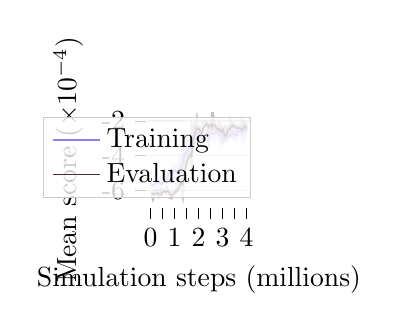
\begin{tikzpicture}

% \begin{axis}[
% axis background/.style={fill=white!82.7450980392157!black},
% axis line style={white},
% legend cell align={left},
% legend style={fill opacity=0.8, draw opacity=1, text opacity=1, at={(1,0.1)}, anchor=south east, draw=white!80!black},
% tick align=outside,
% tick pos=left,
% x grid style={white!69.0196078431373!black},
% xlabel={Simulation steps},
% xmajorgrids,
% xmin=-162030, xmax=4193970,
% xtick style={color=black},
% xtick={-500000,0,500000,1000000,1500000,2000000,2500000,3000000,3500000,4000000,4500000},
% xticklabels={-0.5M,0.0M,0.5M,1.0M,1.5M,2.0M,2.5M,3.0M,3.5M,4.0M,4.5M},
% y grid style={white!69.0196078431373!black},
% ylabel={Mean score},
% ymajorgrids,
% ymin=-7000, ymax=-1500,
% ytick style={color=black}
% ]
\definecolor{color0}{rgb}{0.83921568627451,0.152941176470588,0.156862745098039}
\definecolor{color1}{rgb}{0.12156862745098,0.966666666666667,0.205882352941177}
\definecolor{color2}{rgb}{0.580392156862745,0.503921568627451,0.941176470588235}
\definecolor{color3}{rgb}{0.290196078431372,0.166666666666667,0.23078431372549}

\begin{axis}[
    width=\figurewidth,
    height=\figureheight,
    axis background/.style={fill=white},
    axis line style={white},
    legend cell align={left},
    legend style={fill opacity=0.8, draw opacity=1, text opacity=1, at={(1,0.1)}, anchor=south east, draw=white!80!black},
    tick align=outside,
    tick pos=left,
    x grid style={white},
    xlabel={Simulation steps (millions)},
    xmajorgrids,
    xmin=-162030, 
    xmax=4193970,
    xtick style={color=black},
    xtick={-500000,0,500000,1000000,1500000,2000000,2500000,3000000,3500000,4000000,4500000},
    xticklabels={,0,,1,,2,,3,,4,},
    y grid style={white!80!black},
    ylabel={Mean score ($\times10^{-4}$)},
    ymajorgrids,
    ymin=-7000, 
    ymax=-1500,
    ytick={-10000,-8000,-6000,-4000,-2000},
    yticklabels={-10,-8,-6,-4,-2},
    ytick style={color=black},
    scaled y ticks = false,
    scaled x ticks = false
]
\addplot [ultra thick, color2, opacity=0.3, forget plot]
table {%
35970 -5648.404296875
71970 -5778.49462890625
107970 -5827.8447265625
143970 -5590.2333984375
179970 -5616.9970703125
215970 -5602.96044921875
251970 -5289.59326171875
287970 -5694.8408203125
323970 -5538.4453125
359970 -5645.56787109375
395970 -5566.94970703125
431970 -5776.55908203125
467970 -5635.69775390625
503970 -5588.0927734375
539970 -5464.24365234375
575970 -5498.279296875
611970 -5222.47314453125
647970 -5395.6767578125
683970 -5411.75927734375
719970 -4870.5322265625
755970 -4843.9150390625
791970 -4955.11474609375
827970 -4868.4658203125
863970 -4852.47705078125
899970 -5157.5712890625
935970 -4773.69482421875
971970 -4828.22900390625
1007970 -4710.587890625
1043970 -4858.072265625
1079970 -5280.48779296875
1115970 -5028.30517578125
1151970 -4911.2978515625
1187970 -4556.8466796875
1223970 -5022.69677734375
1259970 -4303.4365234375
1295970 -4020.8720703125
1331970 -4278.50439453125
1367970 -3861.1572265625
1403970 -3914.99072265625
1439970 -3630.04248046875
1475970 -3706.30322265625
1511970 -3753.4189453125
1547970 -3318.51733398438
1583970 -3371.60961914062
1619970 -3479.09350585938
1655970 -3660.86010742188
1691970 -3299.40942382812
1727970 -3428.76318359375
1763970 -2959.56079101562
1799970 -3074.47338867188
1835970 -2524.50463867188
1871970 -2629.50537109375
1907970 -2483.51928710938
1943970 -2581.51196289062
1979970 -2796.37915039062
2015970 -2796.77221679688
2051970 -2788.20190429688
2087970 -2919.04248046875
2123970 -2941.35424804688
2159970 -2906.66943359375
2195970 -2884.07836914062
2231970 -2979.5576171875
2267970 -2847.37719726562
2303970 -2683.82885742188
2339970 -2656.70043945312
2375970 -2682.86694335938
2411970 -2614.64794921875
2447970 -2930.19946289062
2483970 -2774.71875
2519970 -2591.64233398438
2555970 -2798.55590820312
2591970 -2690.65747070312
2627970 -2670.75537109375
2663970 -2841.49633789062
2699970 -2587.88061523438
2735970 -2490.17016601562
2771970 -2621.38061523438
2807970 -2685.76416015625
2843970 -2534.65698242188
2879970 -2440.62060546875
2915970 -2995.59497070312
2951970 -2826.62036132812
2987970 -3034.6533203125
3023970 -2821.01733398438
3059970 -2906.78662109375
3095970 -2679.08813476562
3131970 -3118.02807617188
3167970 -3145.10717773438
3203970 -2901.8837890625
3239970 -2841.25537109375
3275970 -2661.11767578125
3311970 -2787.5703125
3347970 -2722.17822265625
3383970 -2703.61450195312
3419970 -2749.4443359375
3455970 -2722.81640625
3491970 -2698.97924804688
3527970 -2820.46411132812
3563970 -2965.60180664062
3599970 -2789.38061523438
3635970 -2471.5283203125
3671970 -2509.18774414062
3707970 -2436.15307617188
3743970 -2638.46264648438
3779970 -2411.47509765625
3815970 -2721.51879882812
3851970 -2323.9677734375
3887970 -2382.50756835938
3923970 -2736.63061523438
3959970 -2509.34423828125
3995970 -2192.06762695312
};
\addplot [ultra thick, color3, opacity=0.3, forget plot]
table {%
35970 -6195.810546875
71970 -6159.5322265625
107970 -6327.56982421875
143970 -6189.2978515625
179970 -6141.30224609375
215970 -6218.49072265625
251970 -6197.25537109375
287970 -6115.3671875
323970 -6233.5419921875
359970 -6316.56982421875
395970 -6273.86669921875
431970 -6269.11669921875
467970 -6033.8544921875
503970 -6043.43896484375
539970 -6037.75634765625
575970 -6021.943359375
611970 -6166.298828125
647970 -6165.92626953125
683970 -5943.8388671875
719970 -6030.2138671875
755970 -6150.15625
791970 -6327.42822265625
827970 -6386.736328125
863970 -6396.77685546875
899970 -6296.11376953125
935970 -6136.9033203125
971970 -6156.91064453125
1007970 -6029.22998046875
1043970 -5996.6611328125
1079970 -6037.07470703125
1115970 -5979.60107421875
1151970 -5819.0048828125
1187970 -5731.31201171875
1223970 -5455.88330078125
1259970 -5480.69873046875
1295970 -5508.18310546875
1331970 -5824.35302734375
1367970 -5249.046875
1403970 -4952.4248046875
1439970 -4206.19482421875
1475970 -4305.826171875
1511970 -3990.046875
1547970 -4019.04418945312
1583970 -3940.41284179688
1619970 -3993.17041015625
1655970 -3765.69018554688
1691970 -4132.2822265625
1727970 -3428.8876953125
1763970 -2346.04736328125
1799970 -2405.6591796875
1835970 -2640.54125976562
1871970 -2342.4462890625
1907970 -2144.73608398438
1943970 -2558.58715820312
1979970 -2341.31518554688
2015970 -2464.5517578125
2051970 -2706.8662109375
2087970 -2936.2646484375
2123970 -2749.54931640625
2159970 -2408.203125
2195970 -2179.08837890625
2231970 -2225.91064453125
2267970 -2154.49975585938
2303970 -2068.75634765625
2339970 -2139.72045898438
2375970 -2180.9609375
2411970 -2632.62866210938
2447970 -2179.6494140625
2483970 -2159.84838867188
2519970 -2119.74951171875
2555970 -2639.37158203125
2591970 -1900.15234375
2627970 -2196.99975585938
2663970 -2273.89794921875
2699970 -2448.67041015625
2735970 -2551.84130859375
2771970 -2536.00854492188
2807970 -2408.31567382812
2843970 -2596.21752929688
2879970 -2429.89282226562
2915970 -2614.07397460938
2951970 -2734.27490234375
2987970 -2430.45288085938
3023970 -2415.29443359375
3059970 -3077.12451171875
3095970 -3029.80737304688
3131970 -2895.60913085938
3167970 -2658.9833984375
3203970 -2342.75
3239970 -2347.30810546875
3275970 -2367.08081054688
3311970 -2519.51123046875
3347970 -2104.73974609375
3383970 -2184.73901367188
3419970 -2178.01733398438
3455970 -2486.04541015625
3491970 -2276.43090820312
3527970 -2318.30493164062
3563970 -2541.2548828125
3599970 -2471.77392578125
3635970 -2391.25122070312
3671970 -2419.89794921875
3707970 -2360.78979492188
3743970 -2432.16918945312
3779970 -2578.36743164062
3815970 -2638.48608398438
3851970 -2424.4697265625
3887970 -2107.2802734375
3923970 -2167.50610351562
3959970 -2470.2724609375
3995970 -2392.4931640625
};
\addplot [semithick, color2]
table {%
35970 -5648.404296875
71970 -5700.4404296875
107970 -5751.4021484375
143970 -5686.9346484375
179970 -5658.9596171875
215970 -5636.55995
251970 -5497.7732746875
287970 -5576.6002929375
323970 -5561.3383007625
359970 -5595.030128895
395970 -5583.7979601495
431970 -5660.9024089022
467970 -5650.82054690382
503970 -5625.72943751729
539970 -5561.13512344788
575970 -5535.99279281873
611970 -5410.58493350373
647970 -5404.62166322724
683970 -5407.47670887384
719970 -5192.69891594931
755970 -5053.18536519458
791970 -5013.95711755425
827970 -4955.76059865755
863970 -4914.44717950703
899970 -5011.69682332922
935970 -4916.49602368503
971970 -4881.18921577352
1007970 -4812.94868571411
1043970 -4830.99811767847
1079970 -5010.79398779458
1115970 -5017.79846298925
1151970 -4975.19821841855
1187970 -4807.85760292613
1223970 -4893.79327269318
1259970 -4657.65057299091
1295970 -4402.93917191954
1331970 -4353.16526096423
1367970 -4156.36204720354
1403970 -4059.81351738462
1439970 -3887.90510261827
1475970 -3815.26435063346
1511970 -3790.52618850508
1547970 -3601.7226466968
1583970 -3509.67743567433
1619970 -3497.44386374835
1655970 -3562.81036121776
1691970 -3457.4499862619
1727970 -3445.97526519464
1763970 -3251.40947552304
1799970 -3180.63504078257
1835970 -2918.18287993829
1871970 -2802.71187640048
1907970 -2675.03484068404
1943970 -2637.62568956667
1979970 -2701.12707389625
2015970 -2739.3851310565
2051970 -2758.91184035265
2087970 -2822.96409639909
2123970 -2870.3201570582
2159970 -2884.85986767242
2195970 -2884.5472682597
2231970 -2922.55140783082
2267970 -2892.48172360474
2303970 -2809.0205771316
2339970 -2748.09252206021
2375970 -2722.00229057987
2411970 -2679.06055403542
2447970 -2779.5161175775
2483970 -2777.5971705465
2519970 -2703.21523592165
2555970 -2741.35150483424
2591970 -2721.07389118179
2627970 -2700.94648314658
2663970 -2757.1664250442
2699970 -2689.45210112027
2735970 -2609.73932707841
2771970 -2614.3958423408
2807970 -2642.94316946698
2843970 -2599.62869464894
2879970 -2536.02545897686
2915970 -2719.85326366737
2951970 -2762.56010273167
2987970 -2871.397389764
3023970 -2851.24536745215
3059970 -2873.46186890879
3095970 -2795.71237525152
3131970 -2924.63865561966
3167970 -3012.82606446555
3203970 -2968.44915430433
3239970 -2917.5716410201
3275970 -2814.99005492456
3311970 -2804.02215795474
3347970 -2771.28458383534
3383970 -2744.21655108245
3419970 -2746.30766502447
3455970 -2736.91116151468
3491970 -2721.73839612756
3527970 -2761.22868220779
3563970 -2842.97793198092
3599970 -2821.5390052823
3635970 -2681.53473129438
3671970 -2612.59593643288
3707970 -2542.01879232848
3743970 -2580.59633399084
3779970 -2512.947839457
3815970 -2596.37622320545
3851970 -2487.41284329827
3887970 -2445.45073332271
3923970 -2561.92268608738
3959970 -2540.89130696493
3995970 -2401.36183496021
};
\addlegendentry{Training}
\addplot [semithick, color3]
table {%
35970 -6195.810546875
71970 -6181.29921875
107970 -6239.8074609375
143970 -6219.6036171875
179970 -6188.28306875
215970 -6200.3661303125
251970 -6199.121826625
287970 -6165.619970975
323970 -6192.78877946
359970 -6242.3011973635
395970 -6254.9273981056
431970 -6260.60311855086
467970 -6169.90366800552
503970 -6119.31778674081
539970 -6086.69321110699
575970 -6060.79327041419
611970 -6102.99549349851
647970 -6128.16780391161
683970 -6054.43622922196
719970 -6044.74728440818
755970 -6086.91087064491
791970 -6183.11781144944
827970 -6264.56521811967
863970 -6317.4498730593
899970 -6308.91543164808
935970 -6240.11058711385
971970 -6206.83061008081
1007970 -6135.79035823598
1043970 -6080.13866806659
1079970 -6062.91308365245
1115970 -6029.58827987897
1151970 -5945.35492105238
1187970 -5859.73775731893
1223970 -5698.19597470386
1259970 -5611.19707700982
1295970 -5569.99148839339
1331970 -5671.73610397353
1367970 -5502.66041238412
1403970 -5282.56616930547
1439970 -4852.01763127078
1475970 -4633.54104751247
1511970 -4376.14337850748
1547970 -4233.30370288574
1583970 -4116.14735845019
1619970 -4066.95657913262
1655970 -3946.45002169832
1691970 -4020.78290364399
1727970 -3784.0248203114
1763970 -3208.83383749934
1799970 -2887.5639743746
1835970 -2788.75488853101
1871970 -2610.23144874361
1907970 -2424.03330283991
1943970 -2477.8548449852
1979970 -2423.23898120987
2015970 -2439.76409185092
2051970 -2546.60493948555
2087970 -2702.46882306633
2123970 -2721.3010204023
2159970 -2596.06186224138
2195970 -2429.27246890733
2231970 -2347.9277391569
2267970 -2270.55654583789
2303970 -2189.83646656523
2339970 -2169.79006353289
2375970 -2174.25841311973
2411970 -2357.60651271559
2447970 -2286.42367325435
2483970 -2235.79355942136
2519970 -2189.37594034032
2555970 -2369.37419701669
2591970 -2181.68545571001
2627970 -2187.81117576976
2663970 -2222.24588514936
2699970 -2312.81569515211
2735970 -2408.42594052877
2771970 -2459.45898228601
2807970 -2439.00165890286
2843970 -2501.88800706046
2879970 -2473.08993314253
2915970 -2529.48354972927
2951970 -2611.40009077506
2987970 -2539.02120680879
3023970 -2489.53049752277
3059970 -2724.56810320116
3095970 -2846.66381113945
3131970 -2866.24193902742
3167970 -2783.33852279145
3203970 -2607.10311367487
3239970 -2503.18511039242
3275970 -2448.7433904542
3311970 -2477.05052646002
3347970 -2328.12621431351
3383970 -2270.77133405686
3419970 -2233.66973402786
3455970 -2334.62000447922
3491970 -2311.34436596878
3527970 -2314.12859223752
3563970 -2404.97910846751
3599970 -2431.69703539301
3635970 -2415.51870951705
3671970 -2417.27040539773
3707970 -2394.67816120739
3743970 -2409.67457250568
3779970 -2477.15171615966
3815970 -2541.68546328955
3851970 -2494.79916859873
3887970 -2339.79161053424
3923970 -2270.87740772679
3959970 -2350.63542901107
3995970 -2367.37852303164
};
\addlegendentry{Evaluation}
\end{axis}

\end{tikzpicture}
}
            \caption{Base scenario with common perturbation-free environments.}
            \label{fig:base}
        \end{subfigure}
    \end{minipage}
    \begin{minipage}{0.49\textwidth}
        \begin{subfigure}[t]{0.49\textwidth}
            \centering
            \setlength{\figureheight}{0.8\textwidth}
            \setlength{\figurewidth}{\textwidth}
            \scriptsize{% This file was created by tikzplotlib v0.9.1.
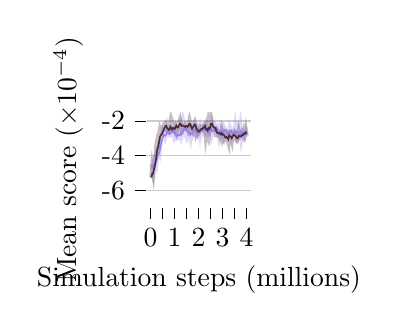
\begin{tikzpicture}

% \begin{axis}[
% axis background/.style={fill=white!82.7450980392157!black},
% axis line style={white},
% legend cell align={left},
% legend style={fill opacity=0.8, draw opacity=1, text opacity=1, at={(1,0.1)}, anchor=south east, draw=white!80!black},
% tick align=outside,
% tick pos=left,
% x grid style={white!69.0196078431373!black},
% xlabel={Simulation steps},
% xmajorgrids,
% xmin=-162030, xmax=4193970,
% xtick style={color=black},
% xtick={-500000,0,500000,1000000,1500000,2000000,2500000,3000000,3500000,4000000,4500000},
% xticklabels={-0.5M,0.0M,0.5M,1.0M,1.5M,2.0M,2.5M,3.0M,3.5M,4.0M,4.5M},
% y grid style={white!69.0196078431373!black},
% ylabel={Mean score},
% ymajorgrids,
% ymin=-7000, ymax=-1500,
% ytick style={color=black}
% ]
\definecolor{color0}{rgb}{0.83921568627451,0.152941176470588,0.156862745098039}
\definecolor{color1}{rgb}{0.12156862745098,0.966666666666667,0.205882352941177}
\definecolor{color2}{rgb}{0.580392156862745,0.503921568627451,0.941176470588235}
\definecolor{color3}{rgb}{0.290196078431372,0.166666666666667,0.23078431372549}

\begin{axis}[
    width=\figurewidth,
    height=\figureheight,
    axis background/.style={fill=white},
    axis line style={white},
    legend cell align={left},
    legend style={fill opacity=0.8, draw opacity=1, text opacity=1, at={(1,0.1)}, anchor=south east, draw=white!80!black},
    tick align=outside,
    tick pos=left,
    x grid style={white},
    xlabel={Simulation steps (millions)},
    xmajorgrids,
    xmin=-162030, 
    xmax=4193970,
    xtick style={color=black},
    xtick={-500000,0,500000,1000000,1500000,2000000,2500000,3000000,3500000,4000000,4500000},
    xticklabels={,0,,1,,2,,3,,4,},
    y grid style={white!80!black},
    ylabel={Mean score ($\times10^{-4}$)},
    ymajorgrids,
    ymin=-7000, 
    ymax=-1500,
    ytick={-10000,-8000,-6000,-4000,-2000},
    yticklabels={-10,-8,-6,-4,-2},
    ytick style={color=black},
    scaled y ticks = false,
    scaled x ticks = false
]
\addplot [ultra thick, color2, opacity=0.3, forget plot]
table {%
35970 -4520.841796875
71970 -4588.193359375
107970 -4860.650390625
143970 -4364.1865234375
179970 -4169.8779296875
215970 -4015.45483398438
251970 -4272.923828125
287970 -3768.5654296875
323970 -3679.40966796875
359970 -3806.92553710938
395970 -3225.55810546875
431970 -2963.62915039062
467970 -2933.8896484375
503970 -2632.4736328125
539970 -2753.49926757812
575970 -2713.35668945312
611970 -2891.25561523438
647970 -2706.24047851562
683970 -2412.72314453125
719970 -2656.80932617188
755970 -2825.55078125
791970 -2829.14453125
827970 -2584.2939453125
863970 -2428.57495117188
899970 -2480.43994140625
935970 -2612.64135742188
971970 -2809.39916992188
1007970 -2599.4072265625
1043970 -2993.16821289062
1079970 -2947.04321289062
1115970 -2892.09252929688
1151970 -2715.54125976562
1187970 -2877.9697265625
1223970 -2796.8291015625
1259970 -2476.60546875
1295970 -2842.07690429688
1331970 -2674.68286132812
1367970 -2158.798828125
1403970 -2424.85107421875
1439970 -2604.45288085938
1475970 -2382.38647460938
1511970 -2382.68530273438
1547970 -2839.19287109375
1583970 -2719.4365234375
1619970 -2771.50537109375
1655970 -2966.23950195312
1691970 -2606.45922851562
1727970 -2724.2666015625
1763970 -2490.03759765625
1799970 -2417.0595703125
1835970 -2416.59521484375
1871970 -2490.71557617188
1907970 -2839.4375
1943970 -2879.17749023438
1979970 -2111.65307617188
2015970 -2487.54833984375
2051970 -2757.69702148438
2087970 -2438.04077148438
2123970 -2624.18310546875
2159970 -2476.10815429688
2195970 -2379.75219726562
2231970 -2546.96313476562
2267970 -2383.81372070312
2303970 -2306.55419921875
2339970 -2715.66186523438
2375970 -2793.31762695312
2411970 -2770.84594726562
2447970 -2544.35302734375
2483970 -2448.60302734375
2519970 -2266.11865234375
2555970 -2787.0146484375
2591970 -2613.10913085938
2627970 -2509.95458984375
2663970 -2447.22216796875
2699970 -2226.22314453125
2735970 -2282.30444335938
2771970 -2577.30688476562
2807970 -2626.70043945312
2843970 -2868.96411132812
2879970 -2505.7333984375
2915970 -2690.47265625
2951970 -2478.52783203125
2987970 -2576.45825195312
3023970 -2767.47216796875
3059970 -2366.6787109375
3095970 -2455.33813476562
3131970 -2632.87646484375
3167970 -2831.68920898438
3203970 -2923.30102539062
3239970 -2711.68823242188
3275970 -2753.26806640625
3311970 -2381.50170898438
3347970 -2495.01708984375
3383970 -2862.52172851562
3419970 -2728.08911132812
3455970 -2681.72802734375
3491970 -2742.92846679688
3527970 -2363.02954101562
3563970 -2736.59790039062
3599970 -2583.7490234375
3635970 -2994.57763671875
3671970 -2915.52709960938
3707970 -2815.1884765625
3743970 -2406.69555664062
3779970 -2885.265625
3815970 -2554.3974609375
3851970 -2598.5830078125
3887970 -2682.32690429688
3923970 -2813.046875
3959970 -2665.92456054688
3995970 -2923.08911132812
};
\addplot [ultra thick, color3, opacity=0.3, forget plot]
table {%
35970 -5273.638671875
71970 -4703.49169921875
107970 -5005.84423828125
143970 -4414.65771484375
179970 -4356.93701171875
215970 -3956.94653320312
251970 -3302.10473632812
287970 -3099.02490234375
323970 -3232.68603515625
359970 -2779.42553710938
395970 -2514.8935546875
431970 -2662.09228515625
467970 -2706.76318359375
503970 -2445.41040039062
539970 -2423.65551757812
575970 -2175.04541015625
611970 -2140.1865234375
647970 -2275.37451171875
683970 -2541.9619140625
719970 -2590.41870117188
755970 -2612.5751953125
791970 -2410.49853515625
827970 -2114.88500976562
863970 -2593.32421875
899970 -2590.14501953125
935970 -2258.61572265625
971970 -2432.71166992188
1007970 -2535.3427734375
1043970 -2165.16064453125
1079970 -2155.41235351562
1115970 -2531.92529296875
1151970 -2377.77880859375
1187970 -2124.12133789062
1223970 -1975.35974121094
1259970 -2243.26831054688
1295970 -2425.49438476562
1331970 -2253.4052734375
1367970 -2277.3759765625
1403970 -2356.83422851562
1439970 -2399.28784179688
1475970 -2221.28515625
1511970 -2270.9189453125
1547970 -2428.15869140625
1583970 -2181.22192382812
1619970 -1968.44396972656
1655970 -2208.1376953125
1691970 -2559.25830078125
1727970 -2623.9091796875
1763970 -2205.08813476562
1799970 -2178.1357421875
1835970 -2077.99340820312
1871970 -2298.23168945312
1907970 -2720.52001953125
1943970 -2596.63989257812
1979970 -2739.29931640625
2015970 -2670.20654296875
2051970 -2512.6533203125
2087970 -2364.7841796875
2123970 -2406.26293945312
2159970 -2463.08081054688
2195970 -2289.37548828125
2231970 -2262.4658203125
2267970 -2189.1279296875
2303970 -2801.43408203125
2339970 -2449.57348632812
2375970 -2665.07446289062
2411970 -2192.05615234375
2447970 -2546.45532226562
2483970 -2207.75268554688
2519970 -1877.70141601562
2555970 -2134.89770507812
2591970 -2453.74780273438
2627970 -2494.10546875
2663970 -2436.92211914062
2699970 -2447.76879882812
2735970 -2820.88232421875
2771970 -2828.28857421875
2807970 -2753.89038085938
2843970 -2697.57006835938
2879970 -2724.0888671875
2915970 -2871.30859375
2951970 -2616.59936523438
2987970 -2922.9130859375
3023970 -2735.62060546875
3059970 -2875.79858398438
3095970 -3086.3271484375
3131970 -3040.94848632812
3167970 -2860.26245117188
3203970 -3002.76025390625
3239970 -3193.2421875
3275970 -2518.17944335938
3311970 -2943.5849609375
3347970 -2944.60595703125
3383970 -3129.71899414062
3419970 -2728.88549804688
3455970 -2666.51953125
3491970 -2850.87963867188
3527970 -2872.64697265625
3563970 -3050.62548828125
3599970 -3105.84912109375
3635970 -2968.66137695312
3671970 -2675.83984375
3707970 -2927.3935546875
3743970 -2881.76928710938
3779970 -2872.4638671875
3815970 -2704.06518554688
3851970 -2823.13940429688
3887970 -2604.19213867188
3923970 -2776.10107421875
3959970 -2527.93432617188
3995970 -2841.0986328125
};
\addplot [semithick, color2]
table {%
35970 -4520.841796875
71970 -4547.782421875
107970 -4672.929609375
143970 -4549.432375
179970 -4397.610596875
215970 -4244.74829171875
251970 -4256.01850628125
287970 -4061.03727564375
323970 -3908.38623257375
359970 -3867.801954388
395970 -3610.9044148203
431970 -3351.99430904843
467970 -3184.75244480406
503970 -2963.84092000743
539970 -2879.70425903571
575970 -2813.16523120268
611970 -2844.40138481536
647970 -2789.13702229546
683970 -2638.57147118978
719970 -2645.86661318262
755970 -2717.74028040957
791970 -2762.30198074574
827970 -2691.09876657245
863970 -2586.08924041222
899970 -2543.82952080983
935970 -2571.35425545465
971970 -2666.57222124154
1007970 -2639.70622336992
1043970 -2781.0910191782
1079970 -2847.47189666317
1115970 -2865.32014971665
1151970 -2805.40859373624
1187970 -2834.43304686675
1223970 -2819.39146874505
1259970 -2682.27706874703
1295970 -2746.19700296697
1331970 -2717.59134631143
1367970 -2494.07433903686
1403970 -2466.38503310961
1439970 -2521.61217220952
1475970 -2465.92189316946
1511970 -2432.62725699543
1547970 -2595.25350263476
1583970 -2644.92671095585
1619970 -2695.55817501101
1655970 -2803.83070578786
1691970 -2724.88211487896
1727970 -2724.63590955238
1763970 -2630.79658479393
1799970 -2545.30177900136
1835970 -2493.81915333831
1871970 -2492.57772247174
1907970 -2631.32163348304
1943970 -2730.46397618358
1979970 -2482.9396161789
2015970 -2484.78310564484
2051970 -2593.94867198065
2087970 -2531.58551178214
2123970 -2568.62454925679
2159970 -2531.61799127282
2195970 -2470.87167366994
2231970 -2501.30825810822
2267970 -2454.31044314618
2303970 -2395.20794557521
2339970 -2523.38951343887
2375970 -2631.36075884457
2411970 -2687.15483421299
2447970 -2630.0341114653
2483970 -2557.46167781668
2519970 -2440.92446762751
2555970 -2579.3605399515
2591970 -2592.85997631465
2627970 -2559.69782172629
2663970 -2514.70756022327
2699970 -2399.31379394647
2735970 -2352.51005371163
2771970 -2442.42878613323
2807970 -2516.13744746119
2843970 -2657.26811300796
2879970 -2596.65422717978
2915970 -2634.18159880787
2951970 -2571.92009209722
2987970 -2573.73535603958
3023970 -2651.23008081125
3059970 -2537.40953286175
3095970 -2504.5809736233
3131970 -2555.89917011148
3167970 -2666.21518566064
3203970 -2769.04952155263
3239970 -2746.10500590033
3275970 -2748.9702301027
3311970 -2601.98282165537
3347970 -2559.19652893072
3383970 -2680.52660876468
3419970 -2699.55160979006
3455970 -2692.42217681154
3491970 -2712.62469280567
3527970 -2572.78663208965
3563970 -2638.31113941004
3599970 -2616.48629302102
3635970 -2767.72283050011
3671970 -2826.84453814382
3707970 -2822.18211351129
3743970 -2655.98749076302
3779970 -2747.69874445781
3815970 -2670.37823104969
3851970 -2641.66014175481
3887970 -2657.92684677164
3923970 -2719.97485806298
3959970 -2698.35473905654
3995970 -2788.24848796517
};
%\addlegendentry{Training}
\addplot [semithick, color3]
table {%
35970 -5273.638671875
71970 -5045.5798828125
107970 -5029.685625
143970 -4783.6744609375
179970 -4612.97948125
215970 -4350.56630203125
251970 -3931.18167575
287970 -3598.3189663875
323970 -3452.065793895
359970 -3183.00969118075
395970 -2915.76323658345
431970 -2814.29485601257
467970 -2771.28218704504
503970 -2640.93347238328
539970 -2554.02229046122
575970 -2402.43153833923
611970 -2297.53353237854
647970 -2288.66992411462
683970 -2389.98672009377
719970 -2470.15951252501
755970 -2527.12578564001
791970 -2480.47488544651
827970 -2334.23893517415
863970 -2437.87304860449
899970 -2498.7818369752
935970 -2402.71539124762
971970 -2414.71390271732
1007970 -2462.96545100539
1043970 -2343.84352841573
1079970 -2268.47105845569
1115970 -2373.85275226091
1151970 -2375.42317479405
1187970 -2274.90244003268
1223970 -2155.08536050398
1259970 -2190.35854052114
1295970 -2284.41287821893
1331970 -2272.00983630636
1367970 -2274.15629240882
1403970 -2307.22746685154
1439970 -2344.05161682967
1475970 -2294.9450325978
1511970 -2285.33459768368
1547970 -2342.46423517271
1583970 -2277.96731063488
1619970 -2154.15797427155
1655970 -2175.74986268793
1691970 -2329.15323792526
1727970 -2447.05561463015
1763970 -2350.26862268434
1799970 -2281.41547048561
1835970 -2200.04664557261
1871970 -2239.32066312482
1907970 -2431.80040568739
1943970 -2497.73620044368
1979970 -2594.36144682871
2015970 -2624.69948528473
2051970 -2579.88101929584
2087970 -2493.8422834525
2123970 -2458.81054585275
2159970 -2460.5186517304
2195970 -2392.06138635074
2231970 -2340.22315993544
2267970 -2279.78506783627
2303970 -2488.44467351426
2339970 -2472.89619863981
2375970 -2549.76750434013
2411970 -2406.68296354158
2447970 -2462.5919070312
2483970 -2360.65621843747
2519970 -2167.47429746873
2555970 -2154.44366051249
2591970 -2274.16531740124
2627970 -2362.14137794075
2663970 -2392.0536744207
2699970 -2414.33972418367
2735970 -2576.9567641977
2771970 -2677.48948820612
2807970 -2708.04984526742
2843970 -2703.8579345042
2879970 -2711.95030757752
2915970 -2775.69362204651
2951970 -2712.05591932166
2987970 -2796.39878596799
3023970 -2772.0875137683
3059970 -2813.57194185473
3095970 -2922.67402448784
3131970 -2969.98380922395
3167970 -2926.09526600312
3203970 -2956.76126116437
3239970 -3051.35363169862
3275970 -2838.08395636292
3311970 -2880.28435819275
3347970 -2906.01299772815
3383970 -2995.49539629314
3419970 -2888.85143699464
3455970 -2799.91867469678
3491970 -2820.30306028682
3527970 -2841.24062523459
3563970 -2924.99457045325
3599970 -2997.33639070945
3635970 -2985.86638520692
3671970 -2861.85576862415
3707970 -2888.07088304949
3743970 -2885.55024467344
3779970 -2880.31569367907
3815970 -2809.81549042619
3851970 -2815.14505597446
3887970 -2730.76388905343
3923970 -2748.89876311956
3959970 -2660.51298834048
3995970 -2732.74724612929
};
%\addlegendentry{Evaluation}
\end{axis}

\end{tikzpicture}
}
            \caption{IF5}
            \label{fig:IF5}
        \end{subfigure}
        \begin{subfigure}[t]{0.49\textwidth}
            \centering
            \setlength{\figureheight}{0.8\textwidth}
            \setlength{\figurewidth}{\textwidth}
            \scriptsize{% This file was created by tikzplotlib v0.9.1.
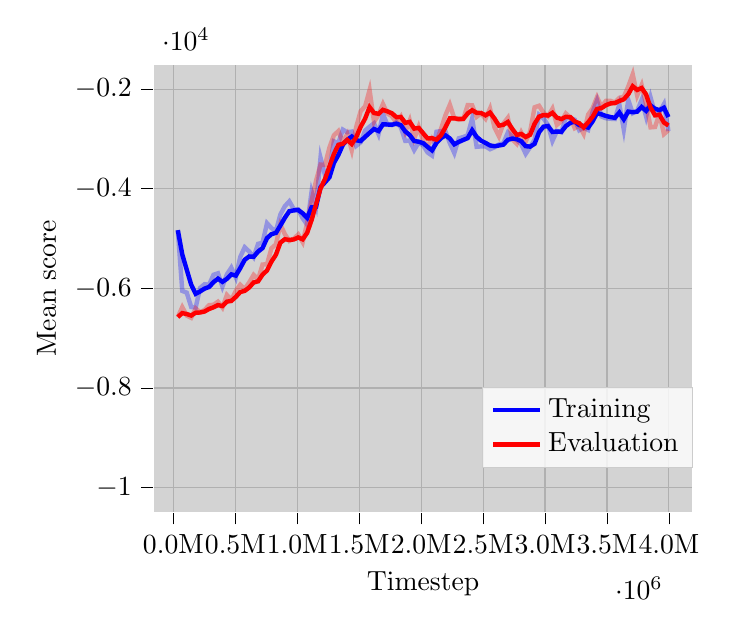
\begin{tikzpicture}

\begin{axis}[
axis background/.style={fill=white!82.7450980392157!black},
axis line style={white},
legend cell align={left},
legend style={fill opacity=0.8, draw opacity=1, text opacity=1, at={(1,0.1)}, anchor=south east, draw=white!80!black},
tick align=outside,
tick pos=left,
x grid style={white!69.0196078431373!black},
xlabel={Timestep},
xmajorgrids,
xmin=-162030, xmax=4193970,
xtick style={color=black},
xtick={-500000,0,500000,1000000,1500000,2000000,2500000,3000000,3500000,4000000,4500000},
xticklabels={-0.5M,0.0M,0.5M,1.0M,1.5M,2.0M,2.5M,3.0M,3.5M,4.0M,4.5M},
y grid style={white!69.0196078431373!black},
ylabel={Mean score},
ymajorgrids,
ymin=-10500, ymax=-1500,
ytick style={color=black}
]
\addplot [ultra thick, blue, opacity=0.3, forget plot]
table {%
35970 -4831.54248046875
71970 -6050.8564453125
107970 -6086.2001953125
143970 -6374.35986328125
179970 -6385.99072265625
215970 -5991.5986328125
251970 -5917.2763671875
287970 -5928.5966796875
323970 -5728.1884765625
359970 -5697.55810546875
395970 -5965.587890625
431970 -5720.681640625
467970 -5584.109375
503970 -5779.08056640625
539970 -5369.61669921875
575970 -5175.3935546875
611970 -5260.259765625
647970 -5374.49853515625
683970 -5106.28076171875
719970 -5084.189453125
755970 -4692.43994140625
791970 -4791.49951171875
827970 -4849.900390625
863970 -4516.984375
899970 -4350.39306640625
935970 -4253.32568359375
971970 -4410.5498046875
1007970 -4415.1962890625
1043970 -4592.60400390625
1079970 -4721.9599609375
1115970 -4055.54077148438
1151970 -4342.302734375
1187970 -3378.2939453125
1223970 -3728.51147460938
1259970 -3617.68896484375
1295970 -3048.3173828125
1331970 -3083.25830078125
1367970 -2813.51806640625
1403970 -2867.52416992188
1439970 -2852.81005859375
1475970 -3138.98486328125
1511970 -3067.44848632812
1547970 -2832.23193359375
1583970 -2755.46020507812
1619970 -2686.55932617188
1655970 -2903.44702148438
1691970 -2504.99853515625
1727970 -2715.53173828125
1763970 -2722.55029296875
1799970 -2662.45141601562
1835970 -2766.59423828125
1871970 -3039.8505859375
1907970 -3032.70166015625
1943970 -3223.37182617188
1979970 -3073.98071289062
2015970 -3128.13110351562
2051970 -3271.53637695312
2087970 -3333.59204101562
2123970 -2856.20751953125
2159970 -2842.80639648438
2195970 -2844.17211914062
2231970 -3086.70947265625
2267970 -3283.05249023438
2303970 -2988.06787109375
2339970 -2962.4287109375
2375970 -2926.52807617188
2411970 -2589.58764648438
2447970 -3157.55249023438
2483970 -3150.28784179688
2519970 -3148.67822265625
2555970 -3207.18481445312
2591970 -3168.42919921875
2627970 -3111.75073242188
2663970 -3089.14111328125
2699970 -2871.93774414062
2735970 -2955.44799804688
2771970 -3022.66430664062
2807970 -3106.46411132812
2843970 -3298.47607421875
2879970 -3165.66967773438
2915970 -3014.16381835938
2951970 -2516.01196289062
2987970 -2588.01245117188
3023970 -2720.625
3059970 -3039.2177734375
3095970 -2840.02978515625
3131970 -2865.95678710938
3167970 -2572.07788085938
3203970 -2581.2041015625
3239970 -2613.83520507812
3275970 -2824.80688476562
3311970 -2773.4306640625
3347970 -2819.5048828125
3383970 -2460.07348632812
3419970 -2227.89184570312
3455970 -2549.64965820312
3491970 -2585.41772460938
3527970 -2595.01098632812
3563970 -2600.04809570312
3599970 -2309.89477539062
3635970 -2810.8544921875
3671970 -2219.29516601562
3707970 -2482.82861328125
3743970 -2436.45043945312
3779970 -2218.75415039062
3815970 -2552.3203125
3851970 -2167.08666992188
3887970 -2494.48583984375
3923970 -2463.08374023438
3959970 -2302.12719726562
3995970 -2841.6630859375
};
\addplot [ultra thick, red, opacity=0.3, forget plot]
table {%
35970 -6576.1904296875
71970 -6377.22705078125
107970 -6545.708984375
143970 -6591.41357421875
179970 -6402.5869140625
215970 -6478.56103515625
251970 -6434.4658203125
287970 -6337.587890625
323970 -6330.97412109375
359970 -6268.19384765625
395970 -6386.35302734375
431970 -6133.541015625
467970 -6229.72412109375
503970 -6052.92138671875
539970 -5926.5537109375
575970 -6014.04443359375
611970 -5882.4208984375
647970 -5730.2626953125
683970 -5823.4765625
719970 -5521.9951171875
755970 -5516.443359375
791970 -5195.048828125
827970 -5116.88427734375
863970 -4718.5400390625
899970 -4912.38818359375
935970 -5048.171875
971970 -5004.43310546875
1007970 -4917.8125
1043970 -5072.2666015625
1079970 -4689.18017578125
1115970 -4239.4580078125
1151970 -3837.84790039062
1187970 -3514.98217773438
1223970 -3523.72021484375
1259970 -3170.83178710938
1295970 -2927.75732421875
1331970 -2842.63549804688
1367970 -3065.44604492188
1403970 -2903.61254882812
1439970 -3225.05688476562
1475970 -2760.08715820312
1511970 -2442.25244140625
1547970 -2346.19409179688
1583970 -2019.08776855469
1619970 -2657.84643554688
1655970 -2517.10595703125
1691970 -2299.05688476562
1727970 -2490.89599609375
1763970 -2542.86157226562
1799970 -2678.76928710938
1835970 -2554.13623046875
1871970 -2854.64038085938
1907970 -2630.0400390625
1943970 -2996.43432617188
1979970 -2756.54833984375
2015970 -3043.60766601562
2051970 -3150.87890625
2087970 -2979.41357421875
2123970 -3054.90991210938
2159970 -2803.32177734375
2195970 -2526.80224609375
2231970 -2313.82690429688
2267970 -2587.32568359375
2303970 -2616.17260742188
2339970 -2600.78466796875
2375970 -2321.3291015625
2411970 -2326.08374023438
2447970 -2556.53295898438
2483970 -2485.87768554688
2519970 -2594.38745117188
2555970 -2391.30883789062
2591970 -2767.50244140625
2627970 -2945.96459960938
2663970 -2691.96850585938
2699970 -2576.046875
2735970 -3009.64331054688
2771970 -3098.54052734375
2807970 -2871.2275390625
2843970 -3051.88208007812
2879970 -2850.64575195312
2915970 -2365.25366210938
2951970 -2334.92407226562
2987970 -2475.25146484375
3023970 -2546.4287109375
3059970 -2394.37744140625
3095970 -2718.22241210938
3131970 -2643.64526367188
3167970 -2489.11279296875
3203970 -2572.4423828125
3239970 -2784.28076171875
3275970 -2734.41186523438
3311970 -2897.7578125
3347970 -2513.32153320312
3383970 -2384.91674804688
3419970 -2162.5205078125
3455970 -2355.79418945312
3491970 -2235.5078125
3527970 -2235.6533203125
3563970 -2269.57958984375
3599970 -2175.91918945312
3635970 -2153.33862304688
3671970 -1950.05407714844
3707970 -1702.85119628906
3743970 -2127.69702148438
3779970 -1919.40063476562
3815970 -2302.08422851562
3851970 -2767.61157226562
3887970 -2760.234375
3923970 -2496.15844726562
3959970 -2903.02856445312
3995970 -2823.84326171875
};
\addplot [ultra thick, blue]
table {%
35970 -4831.54248046875
71970 -5319.26806640625
107970 -5626.04091796875
143970 -5925.36849609375
179970 -6109.61738671875
215970 -6062.40988515625
251970 -6004.35647796875
287970 -5974.05255865625
323970 -5875.70692581875
359970 -5804.44739767875
395970 -5868.90359485725
431970 -5809.61481316435
467970 -5719.41263789861
503970 -5743.27980930167
539970 -5593.8145652685
575970 -5426.4461610361
611970 -5359.97160287166
647970 -5365.7823757855
683970 -5261.9817301588
719970 -5190.86481934528
755970 -4991.49486816967
791970 -4911.4967255893
827970 -4886.85819160358
863970 -4738.90866496215
899970 -4583.50242553979
935970 -4451.43172876137
971970 -4435.07895913182
1007970 -4427.12589110409
1043970 -4493.31713622496
1079970 -4584.77426610997
1115970 -4373.08086825973
1151970 -4360.76961470584
1187970 -3967.77934694851
1223970 -3872.07219801285
1259970 -3770.31890474521
1295970 -3481.51829597213
1331970 -3322.21429789578
1367970 -3118.73580529997
1403970 -3018.25115114873
1439970 -2952.07471412674
1475970 -3026.83877378854
1511970 -3043.08265880438
1547970 -2958.74236872013
1583970 -2877.42950326333
1619970 -2801.08143242674
1655970 -2842.0276680498
1691970 -2707.21601489238
1727970 -2710.54230424793
1763970 -2715.34549973626
1799970 -2694.187866248
1835970 -2723.1504150613
1871970 -2849.83048341178
1907970 -2922.97895410957
1943970 -3043.13610293449
1979970 -3055.47394691694
2015970 -3084.53680955642
2051970 -3159.3366365151
2087970 -3229.03879831531
2123970 -3079.90628680169
2159970 -2985.06633067476
2195970 -2928.70864606111
2231970 -2991.90897669916
2267970 -3108.36638211325
2303970 -3060.24697770545
2339970 -3021.11967099827
2375970 -2983.28303306771
2411970 -2825.80487843438
2447970 -2958.50392315438
2483970 -3035.21749061138
2519970 -3080.60178342933
2555970 -3131.23499583885
2591970 -3146.11267719081
2627970 -3132.36789928323
2663970 -3115.07718488244
2699970 -3017.82140858571
2735970 -2992.87204437018
2771970 -3004.78894927836
2807970 -3045.45901409826
2843970 -3146.66583814646
2879970 -3154.26737398163
2915970 -3098.22595173272
2951970 -2865.34035619588
2987970 -2754.40919418628
3023970 -2740.89551651177
3059970 -2860.22441928206
3095970 -2852.14656563174
3131970 -2857.67065422279
3167970 -2743.43354487743
3203970 -2678.54176755146
3239970 -2652.65914256212
3275970 -2721.51823944352
3311970 -2742.28320929111
3347970 -2773.17187869967
3383970 -2647.93252175105
3419970 -2479.91625133188
3455970 -2507.80961408038
3491970 -2538.85285829198
3527970 -2561.31610950644
3563970 -2576.80890398511
3599970 -2470.04325254732
3635970 -2606.36774840339
3671970 -2451.53871544828
3707970 -2464.05467458147
3743970 -2453.01298053013
3779970 -2359.30944847433
3815970 -2436.5137940846
3851970 -2328.74294441951
3887970 -2395.04010258921
3923970 -2422.25755764727
3959970 -2374.20541349461
3995970 -2561.18848247177
};
\addlegendentry{Training}
\addplot [ultra thick, red]
table {%
35970 -6576.1904296875
71970 -6496.605078125
107970 -6516.246640625
143970 -6546.3134140625
179970 -6488.8228140625
215970 -6484.7181025
251970 -6464.617189625
287970 -6413.805470025
323970 -6380.6729304525
359970 -6335.681297334
395970 -6355.9499893379
431970 -6266.98639985274
467970 -6252.08148834914
503970 -6172.41744769699
539970 -6074.07195299319
575970 -6050.06094523341
611970 -5983.00492651505
647970 -5881.90803403403
683970 -5858.53544542042
719970 -5723.91931412725
755970 -5640.92893222635
791970 -5462.57689058581
827970 -5324.29984528899
863970 -5081.99592279839
899970 -5014.15282711654
935970 -5027.76044626992
971970 -5018.42950994945
1007970 -4978.18270596967
1043970 -5015.8162642068
1079970 -4885.16182883658
1115970 -4626.88030042695
1151970 -4311.26734041242
1187970 -3992.7532753412
1223970 -3805.14005114222
1259970 -3551.41674552908
1295970 -3301.95297700495
1331970 -3118.22598542172
1367970 -3097.11400922178
1403970 -3019.71342506432
1439970 -3101.85080894484
1475970 -2965.14534864815
1511970 -2755.98818575139
1547970 -2592.07054816959
1583970 -2362.87743632363
1619970 -2480.86503601293
1655970 -2495.36140442026
1691970 -2416.8395965584
1727970 -2446.46215637254
1763970 -2485.02192272978
1799970 -2562.52086848162
1835970 -2559.16701327647
1871970 -2677.35636030963
1907970 -2658.42983181078
1943970 -2793.63162955522
1979970 -2778.79831367063
2015970 -2884.72205460863
2051970 -2991.18479526518
2087970 -2986.47630684661
2123970 -3013.84974895171
2159970 -2929.63856030853
2195970 -2768.50403462262
2231970 -2586.63318249232
2267970 -2586.91018293289
2303970 -2598.61515272849
2339970 -2599.48295882459
2375970 -2488.22141591975
2411970 -2423.3663456456
2447970 -2476.63299098111
2483970 -2480.33086880742
2519970 -2525.9535017532
2555970 -2472.09563620817
2591970 -2590.2583582874
2627970 -2732.54085481619
2663970 -2716.31191523346
2699970 -2660.20589914008
2735970 -2799.9808637028
2771970 -2919.40472915918
2807970 -2900.13385312051
2843970 -2960.83314390355
2879970 -2916.75818712338
2915970 -2696.15637711778
2951970 -2551.66345517692
2987970 -2521.09865904365
3023970 -2531.23067980119
3059970 -2476.48938444321
3095970 -2573.18259550968
3131970 -2601.36766277456
3167970 -2556.46571485223
3203970 -2562.85638203634
3239970 -2651.4261339093
3275970 -2684.62042643933
3311970 -2769.8753808636
3347970 -2667.25384179941
3383970 -2554.3190042984
3419970 -2397.59960570404
3455970 -2380.87743920367
3491970 -2322.7295885222
3527970 -2287.89908123832
3563970 -2280.57128468049
3599970 -2238.71044658955
3635970 -2204.56171717248
3671970 -2102.75866116286
3707970 -1942.79567521334
3743970 -2016.75621372176
3779970 -1977.8139821393
3815970 -2107.52208068983
3851970 -2371.55787732015
3887970 -2527.02847639209
3923970 -2514.6804647415
3959970 -2670.01970462615
3995970 -2731.54912746319
};
\addlegendentry{Evaluation}
\end{axis}

\end{tikzpicture}
}
            \caption{IF15}
            \label{fig:IF15}
        \end{subfigure}
        \begin{subfigure}[t]{0.49\textwidth}
            \centering
            \setlength{\figureheight}{0.8\textwidth}
            \setlength{\figurewidth}{\textwidth}
            \scriptsize{% This file was created by tikzplotlib v0.9.1.
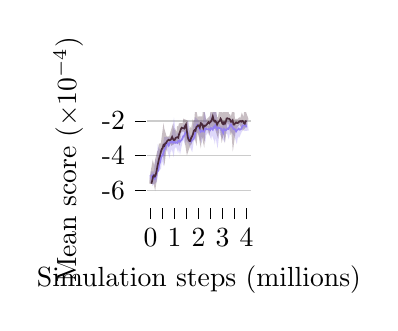
\begin{tikzpicture}

% \begin{axis}[
% axis background/.style={fill=white!82.7450980392157!black},
% axis line style={white},
% legend cell align={left},
% legend style={fill opacity=0.8, draw opacity=1, text opacity=1, at={(1,0.1)}, anchor=south east, draw=white!80!black},
% tick align=outside,
% tick pos=left,
% x grid style={white!69.0196078431373!black},
% xlabel={Simulation steps},
% xmajorgrids,
% xmin=-162030, xmax=4193970,
% xtick style={color=black},
% xtick={-500000,0,500000,1000000,1500000,2000000,2500000,3000000,3500000,4000000,4500000},
% xticklabels={-0.5M,0.0M,0.5M,1.0M,1.5M,2.0M,2.5M,3.0M,3.5M,4.0M,4.5M},
% y grid style={white!69.0196078431373!black},
% ylabel={Mean score},
% ymajorgrids,
% ymin=-7000, ymax=-1500,
% ytick style={color=black}
% ]
\definecolor{color0}{rgb}{0.83921568627451,0.152941176470588,0.156862745098039}
\definecolor{color1}{rgb}{0.12156862745098,0.966666666666667,0.205882352941177}
\definecolor{color2}{rgb}{0.580392156862745,0.503921568627451,0.941176470588235}
\definecolor{color3}{rgb}{0.290196078431372,0.166666666666667,0.23078431372549}

\begin{axis}[
    width=\figurewidth,
    height=\figureheight,
    axis background/.style={fill=white},
    axis line style={white},
    legend cell align={left},
    legend style={fill opacity=0.8, draw opacity=1, text opacity=1, at={(1,0.1)}, anchor=south east, draw=white!80!black},
    tick align=outside,
    tick pos=left,
    x grid style={white},
    xlabel={Simulation steps (millions)},
    xmajorgrids,
    xmin=-162030, 
    xmax=4193970,
    xtick style={color=black},
    xtick={-500000,0,500000,1000000,1500000,2000000,2500000,3000000,3500000,4000000,4500000},
    xticklabels={,0,,1,,2,,3,,4,},
    y grid style={white!80!black},
    ylabel={Mean score ($\times10^{-4}$)},
    ymajorgrids,
    ymin=-7000, 
    ymax=-1500,
    ytick={-10000,-8000,-6000,-4000,-2000},
    yticklabels={-10,-8,-6,-4,-2},
    ytick style={color=black},
    scaled y ticks = false,
    scaled x ticks = false
]
\addplot [ultra thick, color2, opacity=0.3, forget plot]
table {%
35970 -5117.69970703125
71970 -5566.61181640625
107970 -4929.26220703125
143970 -5499.67333984375
179970 -5458.34423828125
215970 -5087.70654296875
251970 -4675.86767578125
287970 -4794.30615234375
323970 -4750.7705078125
359970 -4019.09423828125
395970 -4175.88623046875
431970 -3783.71899414062
467970 -3804.07739257812
503970 -3973.36401367188
539970 -3539.08056640625
575970 -3427.9580078125
611970 -3422.56103515625
647970 -3061.40625
683970 -3065.36791992188
719970 -3399.5400390625
755970 -3556.74658203125
791970 -3097.1953125
827970 -3068.22534179688
863970 -3296.52319335938
899970 -3133.69555664062
935970 -3348.39526367188
971970 -2926.91479492188
1007970 -3383.4638671875
1043970 -3315.64233398438
1079970 -3183.53955078125
1115970 -3323.31469726562
1151970 -3000.82763671875
1187970 -3083.32153320312
1223970 -3310.4482421875
1259970 -3056.87866210938
1295970 -3015.7177734375
1331970 -2870.54931640625
1367970 -2679.11328125
1403970 -2835.0400390625
1439970 -2506.81811523438
1475970 -2576.3388671875
1511970 -2461.30126953125
1547970 -3010.27758789062
1583970 -3117.93603515625
1619970 -3164.52661132812
1655970 -3218.79248046875
1691970 -3336.14477539062
1727970 -2999.83813476562
1763970 -3025.4111328125
1799970 -2928.8955078125
1835970 -2612.88549804688
1871970 -2181.25610351562
1907970 -2016.48901367188
1943970 -2063.65087890625
1979970 -2432.05102539062
2015970 -2590.4423828125
2051970 -2640.5810546875
2087970 -2786.18872070312
2123970 -2474.31201171875
2159970 -2657.47631835938
2195970 -2524.50561523438
2231970 -2668.51416015625
2267970 -2175.42333984375
2303970 -2427.80249023438
2339970 -2554.85595703125
2375970 -2484.30932617188
2411970 -2446.78955078125
2447970 -2476.36547851562
2483970 -2598.67993164062
2519970 -2230.65112304688
2555970 -2473.36254882812
2591970 -2601.06640625
2627970 -2134.84326171875
2663970 -2446.15185546875
2699970 -2029.83801269531
2735970 -2430.79345703125
2771970 -2712.97290039062
2807970 -2270.22631835938
2843970 -2353.71484375
2879970 -2487.65649414062
2915970 -2450.34643554688
2951970 -2496.40112304688
2987970 -2749.9873046875
3023970 -2833.85668945312
3059970 -2132.7314453125
3095970 -2573.56396484375
3131970 -2590.04809570312
3167970 -2452.54296875
3203970 -2328
3239970 -2506.25708007812
3275970 -2243.86694335938
3311970 -2113.15869140625
3347970 -2081.20190429688
3383970 -2406.5869140625
3419970 -2520.25366210938
3455970 -2594.21069335938
3491970 -2470.15405273438
3527970 -2571.30200195312
3563970 -2744.19262695312
3599970 -2401.6669921875
3635970 -2421.8994140625
3671970 -2368.88061523438
3707970 -2598.89282226562
3743970 -2486.97412109375
3779970 -2387.5478515625
3815970 -2128.21752929688
3851970 -2152.44580078125
3887970 -2249.71533203125
3923970 -2263.99975585938
3959970 -2204.29809570312
3995970 -2567.16552734375
};
\addplot [ultra thick, color3, opacity=0.3, forget plot]
table {%
35970 -5628.083984375
71970 -5139.68408203125
107970 -4855.955078125
143970 -5057.69873046875
179970 -5311.10302734375
215970 -4984.681640625
251970 -4532.38525390625
287970 -4207.5205078125
323970 -4035.01000976562
359970 -3814.32104492188
395970 -3788.9013671875
431970 -3420.12109375
467970 -3411.97045898438
503970 -3485.94946289062
539970 -3110.95922851562
575970 -3511.10302734375
611970 -3076.82495117188
647970 -3248.55322265625
683970 -3023.25219726562
719970 -3045.92260742188
755970 -3024.78759765625
791970 -3165.74584960938
827970 -3073.68090820312
863970 -2934.90405273438
899970 -2765.8310546875
935970 -3216.38012695312
971970 -3182.70361328125
1007970 -3089.0830078125
1043970 -2813.2841796875
1079970 -2916.10815429688
1115970 -2919.66186523438
1151970 -3007.05786132812
1187970 -2449.05322265625
1223970 -2458.15600585938
1259970 -2252.12036132812
1295970 -2246.36938476562
1331970 -2449.31909179688
1367970 -2411.25537109375
1403970 -2466.8857421875
1439970 -2052.31274414062
1475970 -2074.95141601562
1511970 -3137.82788085938
1547970 -3456.9033203125
1583970 -3309.84936523438
1619970 -3285.07958984375
1655970 -3142.37524414062
1691970 -2697.19897460938
1727970 -2783.26953125
1763970 -2595.59301757812
1799970 -2314.64721679688
1835970 -2416.63842773438
1871970 -2626.98291015625
1907970 -2031.828125
1943970 -2274.41186523438
1979970 -2140.25952148438
2015970 -2284.39868164062
2051970 -2553.57763671875
2087970 -1742.37963867188
2123970 -2153.4365234375
2159970 -2412.8388671875
2195970 -2652.96508789062
2231970 -2046.41662597656
2267970 -2328.9619140625
2303970 -2194.7734375
2339970 -2138.64819335938
2375970 -2019.46533203125
2411970 -1970.86975097656
2447970 -2226.6708984375
2483970 -2001.20190429688
2519970 -1920.57788085938
2555970 -1744.34936523438
2591970 -1485.04418945312
2627970 -2206.11499023438
2663970 -2181.77661132812
2699970 -1945.79272460938
2735970 -2225.36840820312
2771970 -2391.32299804688
2807970 -1927.47265625
2843970 -1946.77783203125
2879970 -1941.63903808594
2915970 -1663.69689941406
2951970 -2042.84033203125
2987970 -2472.00146484375
3023970 -2225.5966796875
3059970 -1904.51501464844
3095970 -2291.05395507812
3131970 -1904.42028808594
3167970 -1548.81823730469
3203970 -1825.98486328125
3239970 -1921.07153320312
3275970 -1854.0703125
3311970 -1993.99645996094
3347970 -2249.92333984375
3383970 -2053.61450195312
3419970 -1850.50207519531
3455970 -2551.74340820312
3491970 -2195.9697265625
3527970 -2012.11303710938
3563970 -2012.20141601562
3599970 -2183.654296875
3635970 -2105.6533203125
3671970 -1996.03649902344
3707970 -1947.98596191406
3743970 -1982.50854492188
3779970 -2097.51489257812
3815970 -1916.29565429688
3851970 -2042.16015625
3887970 -2279.1640625
3923970 -2210.27587890625
3959970 -1804.39172363281
3995970 -1948.78283691406
};
\addplot [semithick, color2]
table {%
35970 -5117.69970703125
71970 -5297.26455078125
107970 -5150.06361328125
143970 -5289.90750390625
179970 -5357.28219765625
215970 -5249.45193578125
251970 -5020.01823178125
287970 -4929.73340000625
323970 -4858.14824312875
359970 -4522.52664118975
395970 -4383.87047690135
431970 -4143.80988379706
467970 -4007.91688730949
503970 -3994.09573785444
539970 -3812.08966927516
575970 -3658.4370046901
611970 -3564.08661687656
647970 -3363.01447012594
683970 -3243.95585004431
719970 -3306.18952565159
755970 -3406.41234820345
791970 -3282.72553392207
827970 -3196.92545707199
863970 -3236.76455158695
899970 -3195.53695360842
935970 -3256.6802776338
971970 -3124.77408454903
1007970 -3228.24999760442
1043970 -3263.2069321564
1079970 -3231.33997960634
1115970 -3268.12986667005
1151970 -3161.20897468953
1187970 -3130.05399809497
1223970 -3202.21169573198
1259970 -3144.07848228294
1295970 -3092.73419874476
1331970 -3003.86024580936
1367970 -2873.96145998561
1403970 -2858.39289161637
1439970 -2717.76298106357
1475970 -2661.19333551314
1511970 -2581.23650912039
1547970 -2752.85294062848
1583970 -2898.88617843959
1619970 -3005.142351595
1655970 -3090.6024031445
1691970 -3188.81935204295
1727970 -3113.22686513202
1763970 -3078.10057220421
1799970 -3018.41854644753
1835970 -2856.20532708727
1871970 -2586.22563765861
1907970 -2358.33098806392
1943970 -2240.45894440085
1979970 -2317.09577679676
2015970 -2426.43441920306
2051970 -2512.09307339683
2087970 -2621.73133231935
2123970 -2562.76360407911
2159970 -2600.64868979122
2195970 -2570.19145996848
2231970 -2609.52054004359
2267970 -2435.88165996365
2303970 -2432.64999207194
2339970 -2481.53237805566
2375970 -2482.64315730215
2411970 -2468.30171469379
2447970 -2471.52722022252
2483970 -2522.38830478976
2519970 -2405.69343209261
2555970 -2432.76107878682
2591970 -2500.08320977209
2627970 -2353.98723055075
2663970 -2390.85308051795
2699970 -2246.4470533889
2735970 -2320.18561484584
2771970 -2477.30052906375
2807970 -2394.470844782
2843970 -2378.1684443692
2879970 -2421.96366427777
2915970 -2433.31677278541
2951970 -2458.55051289
2987970 -2575.125229609
3023970 -2678.61781354665
3059970 -2460.26326625299
3095970 -2505.58354568929
3131970 -2539.36936569483
3167970 -2504.6388069169
3203970 -2433.98328415014
3239970 -2462.89280252133
3275970 -2375.28245885655
3311970 -2270.43295187643
3347970 -2194.74053284461
3383970 -2279.47908533176
3419970 -2375.78891604281
3455970 -2463.15762696944
3491970 -2465.95619727541
3527970 -2508.0945191465
3563970 -2602.53376226915
3599970 -2522.18705423649
3635970 -2482.07199816689
3671970 -2436.79544499389
3707970 -2501.63439590258
3743970 -2495.77028597905
3779970 -2452.48131221243
3815970 -2322.77579904621
3851970 -2254.64379974022
3887970 -2252.67241265663
3923970 -2257.20334993773
3959970 -2236.04124824389
3995970 -2368.49095988383
};
%\addlegendentry{Training}
\addplot [semithick, color3]
table {%
35970 -5628.083984375
71970 -5432.7240234375
107970 -5202.0164453125
143970 -5144.289359375
179970 -5211.0148265625
215970 -5120.4815521875
251970 -4885.243032875
287970 -4614.15402285
323970 -4382.49641761625
359970 -4155.2262685385
395970 -4008.6963079981
431970 -3773.26622229886
467970 -3628.74791697307
503970 -3571.62853534009
539970 -3387.3608126103
575970 -3436.85769850368
611970 -3292.84459957096
647970 -3275.12804880508
683970 -3174.37770818929
719970 -3122.99566788233
755970 -3083.7124397919
791970 -3116.52580371889
827970 -3099.38784551258
863970 -3033.5943284013
899970 -2926.48901891578
935970 -3042.44546213072
971970 -3098.54872259093
1007970 -3094.76243667956
1043970 -2982.17113388274
1079970 -2955.74594204839
1115970 -2941.31231132278
1151970 -2967.61053132492
1187970 -2760.18760785745
1223970 -2639.37496705822
1259970 -2484.47312476618
1295970 -2389.23162876596
1331970 -2413.26661397833
1367970 -2412.4621168245
1403970 -2434.2315669697
1439970 -2281.46403783807
1475970 -2198.85898910909
1511970 -2574.4465458092
1547970 -2927.42925561052
1583970 -3080.39729946006
1619970 -3162.27021561354
1655970 -3154.31222702437
1691970 -2971.46692605837
1727970 -2896.18796813502
1763970 -2775.94998791226
1799970 -2591.42887946611
1835970 -2521.51269877342
1871970 -2563.70078332655
1907970 -2350.95171999593
1943970 -2320.33577809131
1979970 -2248.30527544853
2015970 -2262.74263792537
2051970 -2379.07663744272
2087970 -2124.39783793438
2123970 -2136.01331213563
2159970 -2246.74353415638
2195970 -2409.23215565008
2231970 -2264.10594378067
2267970 -2290.0483318934
2303970 -2251.93837413604
2339970 -2206.62230182537
2375970 -2131.75951390772
2411970 -2067.40360873526
2447970 -2131.11052461616
2483970 -2079.14707648844
2519970 -2015.71939823682
2555970 -1907.17138503584
2591970 -1738.32050680275
2627970 -1925.4383001754
2663970 -2027.97362463649
2699970 -1995.10126462564
2735970 -2087.20812205664
2771970 -2208.85407245273
2807970 -2096.30150597164
2843970 -2036.49203639548
2879970 -1998.55083707167
2915970 -1864.60926200862
2951970 -1935.90169001767
2987970 -2150.3415999481
3023970 -2180.44363184386
3059970 -2070.07218496569
3095970 -2158.46489301067
3131970 -2056.84705104077
3167970 -1853.63552554634
3203970 -1842.5752606403
3239970 -1873.97376966543
3275970 -1866.01238679926
3311970 -1917.20601606393
3347970 -2050.29294557586
3383970 -2051.62156812676
3419970 -1971.17377095418
3455970 -2203.40162585376
3491970 -2200.42886613726
3527970 -2125.1025345261
3563970 -2079.94208712191
3599970 -2121.42697102315
3635970 -2115.11751073889
3671970 -2067.48510605271
3707970 -2019.68544839725
3743970 -2004.8146870071
3779970 -2041.89476923551
3815970 -1991.65512326006
3851970 -2011.85713645603
3887970 -2118.77990687362
3923970 -2155.37829568667
3959970 -2014.98366686513
3995970 -1988.5033348847
};
%\addlegendentry{Evaluation}
\end{axis}

\end{tikzpicture}
}
            \caption{IF25}
            \label{fig:IF25}
        \end{subfigure}
        \begin{subfigure}[t]{0.49\textwidth}
            \centering
            \setlength{\figureheight}{0.8\textwidth}
            \setlength{\figurewidth}{\textwidth}
            \scriptsize{% This file was created by tikzplotlib v0.9.1.
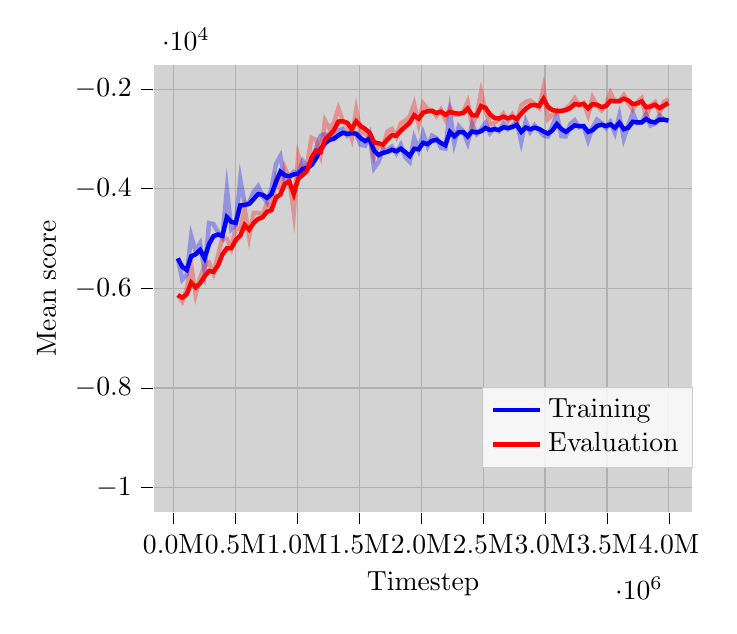
\begin{tikzpicture}

\begin{axis}[
axis background/.style={fill=white!82.7450980392157!black},
axis line style={white},
legend cell align={left},
legend style={fill opacity=0.8, draw opacity=1, text opacity=1, at={(1,0.1)}, anchor=south east, draw=white!80!black},
tick align=outside,
tick pos=left,
x grid style={white!69.0196078431373!black},
xlabel={Timestep},
xmajorgrids,
xmin=-162030, xmax=4193970,
xtick style={color=black},
xtick={-500000,0,500000,1000000,1500000,2000000,2500000,3000000,3500000,4000000,4500000},
xticklabels={-0.5M,0.0M,0.5M,1.0M,1.5M,2.0M,2.5M,3.0M,3.5M,4.0M,4.5M},
y grid style={white!69.0196078431373!black},
ylabel={Mean score},
ymajorgrids,
ymin=-10500, ymax=-1500,
ytick style={color=black}
]
\addplot [ultra thick, blue, opacity=0.3, forget plot]
table {%
35970 -5397.76611328125
71970 -5824.9013671875
107970 -5723.8037109375
143970 -4944.7802734375
179970 -5255.31982421875
215970 -5101.119140625
251970 -5641.43115234375
287970 -4688.32568359375
323970 -4710.71142578125
359970 -4869.775390625
395970 -4984.66845703125
431970 -4008.50390625
467970 -4809.35595703125
503970 -4713.62841796875
539970 -3809.2607421875
575970 -4312.02197265625
611970 -4269.966796875
647970 -4065.32983398438
683970 -3950.8896484375
719970 -4146.78466796875
755970 -4275.75830078125
791970 -3997.00537109375
827970 -3507.30810546875
863970 -3344.3037109375
899970 -3841.6962890625
935970 -3772.49951171875
971970 -3659.53735351562
1007970 -3688.72314453125
1043970 -3443.06396484375
1079970 -3567.14990234375
1115970 -3425.93212890625
1151970 -3184.6337890625
1187970 -2935.11206054688
1223970 -2908.60986328125
1259970 -2917.2001953125
1295970 -2959.74145507812
1331970 -2831.02075195312
1367970 -2798.50830078125
1403970 -2933.54858398438
1439970 -2863.06494140625
1475970 -2908.60717773438
1511970 -3118.26098632812
1547970 -3135.83911132812
1583970 -2920.68774414062
1619970 -3587.20263671875
1655970 -3461.41943359375
1691970 -3213.91845703125
1727970 -3228.37329101562
1763970 -3154.19702148438
1799970 -3291.01147460938
1835970 -3120.61840820312
1871970 -3366.9599609375
1907970 -3459.7275390625
1943970 -2982.75219726562
1979970 -3222.02954101562
2015970 -2887.15161132812
2051970 -3145.95361328125
2087970 -2936.28735351562
2123970 -2984.25634765625
2159970 -3179.91455078125
2195970 -3194.86499023438
2231970 -2457.51196289062
2267970 -3081.41796875
2303970 -2747.14208984375
2339970 -2852.1904296875
2375970 -3080.21850585938
2411970 -2701.78857421875
2447970 -2903.10717773438
2483970 -2807.80249023438
2519970 -2681.08642578125
2555970 -2883.07006835938
2591970 -2780.32958984375
2627970 -2843.0146484375
2663970 -2687.13549804688
2699970 -2803.33422851562
2735970 -2733.8642578125
2771970 -2654.15649414062
2807970 -3062.13525390625
2843970 -2643.23095703125
2879970 -2859.06469726562
2915970 -2724.53588867188
2951970 -2835.53100585938
2987970 -2933.85986328125
3023970 -2952.52709960938
3059970 -2734.47436523438
3095970 -2513.20458984375
3131970 -2947.15869140625
3167970 -2947.41064453125
3203970 -2699.8427734375
3239970 -2627.8876953125
3275970 -2769.1630859375
3311970 -2745.16186523438
3347970 -3029.08227539062
3383970 -2770.43237304688
3419970 -2613.57666015625
3455970 -2677.64721679688
3491970 -2781.5830078125
3527970 -2659.81591796875
3563970 -2878.40844726562
3599970 -2529.07958984375
3635970 -2993.85205078125
3671970 -2729.80590820312
3707970 -2479.51489257812
3743970 -2683.43334960938
3779970 -2667.57592773438
3815970 -2503.2568359375
3851970 -2731.50732421875
3887970 -2690.91015625
3923970 -2529.02978515625
3959970 -2615.31372070312
3995970 -2649.16186523438
};
\addplot [ultra thick, red, opacity=0.3, forget plot]
table {%
35970 -6135.1044921875
71970 -6262.51708984375
107970 -6017.85888671875
143970 -5531.94189453125
179970 -6122.66357421875
215970 -5784.6552734375
251970 -5549.47509765625
287970 -5485.6572265625
323970 -5696.5732421875
359970 -5348.2138671875
395970 -4982.5576171875
431970 -5009.08056640625
467970 -5193.3857421875
503970 -4777.470703125
539970 -4811.62939453125
575970 -4400.955078125
611970 -4964.40380859375
647970 -4486.35302734375
683970 -4486.52783203125
719970 -4518.92138671875
755970 -4297.1240234375
791970 -4377.44189453125
827970 -3805.82006835938
863970 -4016.26611328125
899970 -3582.90771484375
935970 -3795.1083984375
971970 -4478.3193359375
1007970 -3328.20458984375
1043970 -3619.55590820312
1079970 -3504.43237304688
1115970 -2978.04809570312
1151970 -3024.61499023438
1187970 -3315.2646484375
1223970 -2631.73315429688
1259970 -2791.87060546875
1295970 -2674.69555664062
1331970 -2388.17504882812
1367970 -2642.36157226562
1403970 -2721.48706054688
1439970 -2986.05322265625
1475970 -2416.05834960938
1511970 -2886.00390625
1547970 -2886.72534179688
1583970 -2984.13012695312
1619970 -3362.13793945312
1655970 -3114.00659179688
1691970 -3160.7978515625
1727970 -2851.890625
1763970 -2800.45556640625
1799970 -2950.8203125
1835970 -2687.63671875
1871970 -2631.76196289062
1907970 -2552.01391601562
1943970 -2301.97119140625
1979970 -2699.79150390625
2015970 -2290.90380859375
2051970 -2402.5205078125
2087970 -2426.36645507812
2123970 -2541.81176757812
2159970 -2412.48071289062
2195970 -2608.5849609375
2231970 -2373.10229492188
2267970 -2517.07495117188
2303970 -2510.37524414062
2339970 -2460.35961914062
2375970 -2255.05590820312
2411970 -2727.37231445312
2447970 -2533.22143554688
2483970 -2058.44287109375
2519970 -2433.56567382812
2555970 -2703.5166015625
2591970 -2682.40112304688
2627970 -2611.73999023438
2663970 -2494.19555664062
2699970 -2640.43212890625
2735970 -2508.57739257812
2771970 -2667.72387695312
2807970 -2329.4052734375
2843970 -2257.10107421875
2879970 -2228.2275390625
2915970 -2297.28344726562
2951970 -2376.06567382812
2987970 -1978.203125
3023970 -2599.5380859375
3059970 -2517.42602539062
3095970 -2458.29223632812
3131970 -2443.2578125
3167970 -2394.24731445312
3203970 -2314.50756835938
3239970 -2186.07006835938
3275970 -2328.79931640625
3311970 -2275.859375
3347970 -2520.69213867188
3383970 -2170.54028320312
3419970 -2336.03930664062
3455970 -2426.5869140625
3491970 -2313.95288085938
3527970 -2076.42919921875
3563970 -2251.93017578125
3599970 -2243.17529296875
3635970 -2119.73657226562
3671970 -2277.43310546875
3707970 -2409.82958984375
3743970 -2268.65454101562
3779970 -2184.08178710938
3815970 -2541.43041992188
3851970 -2327.8984375
3887970 -2261.70458984375
3923970 -2477.49096679688
3959970 -2255.99340820312
3995970 -2200.1025390625
};
\addplot [ultra thick, blue]
table {%
35970 -5397.76611328125
71970 -5568.62021484375
107970 -5630.69361328125
143970 -5356.32827734375
179970 -5315.92489609375
215970 -5230.00259390625
251970 -5394.57401728125
287970 -5112.07468380625
323970 -4951.52938059625
359970 -4918.82778460775
395970 -4945.16405357715
431970 -4570.49999464629
467970 -4666.04237960027
503970 -4685.07679494766
539970 -4334.7503738436
575970 -4325.65901336866
611970 -4303.3821267712
647970 -4208.16120965647
683970 -4105.25258516888
719970 -4121.86541828883
755970 -4183.4225712858
791970 -4108.85569120898
827970 -3868.23665691289
863970 -3658.66347852273
899970 -3731.87660273864
935970 -3748.12576633068
971970 -3712.69040120466
1007970 -3703.1034985353
1043970 -3599.08768505868
1079970 -3586.31257197271
1115970 -3522.16039474612
1151970 -3387.14975247267
1187970 -3206.33467570235
1223970 -3087.24475073391
1259970 -3019.22692856535
1295970 -2995.43273917046
1331970 -2929.66794428352
1367970 -2877.20408688261
1403970 -2899.74188572332
1439970 -2885.07110799649
1475970 -2894.48553589164
1511970 -2983.99571606624
1547970 -3044.73307417099
1583970 -2995.11494215885
1619970 -3231.95001998281
1655970 -3323.73778542718
1691970 -3279.81005406881
1727970 -3259.23534884754
1763970 -3217.22001790227
1799970 -3246.73660058511
1835970 -3196.28932363232
1871970 -3264.55757855439
1907970 -3342.62556275763
1943970 -3198.67621656083
1979970 -3208.01754634275
2015970 -3079.6711723369
2051970 -3106.18414871464
2087970 -3038.22543063503
2123970 -3016.63779744352
2159970 -3081.94849877861
2195970 -3127.11509536092
2231970 -2859.2738423728
2267970 -2948.13149292368
2303970 -2867.73573169171
2339970 -2861.51761089003
2375970 -2948.99796887776
2411970 -2850.11421101416
2447970 -2871.31139770225
2483970 -2845.9078347151
2519970 -2779.97927114156
2555970 -2821.21559002869
2591970 -2804.86118995471
2627970 -2820.12257334783
2663970 -2766.92774322745
2699970 -2781.49033734272
2735970 -2762.43990553063
2771970 -2719.12654097463
2807970 -2856.33002614728
2843970 -2771.09039850087
2879970 -2806.28011800677
2915970 -2773.58242627281
2951970 -2798.36185810744
2987970 -2852.56106017696
3023970 -2892.54747594993
3059970 -2829.31823166371
3095970 -2702.87277493572
3131970 -2800.58714152393
3167970 -2859.31654272686
3203970 -2795.52703501112
3239970 -2728.47129913167
3275970 -2744.748013854
3311970 -2744.91355440615
3347970 -2858.58104279994
3383970 -2823.32157489871
3419970 -2739.42360900173
3455970 -2714.71305211979
3491970 -2741.46103439687
3527970 -2708.80298782562
3563970 -2776.64517160162
3599970 -2677.61893889847
3635970 -2804.11218365158
3671970 -2774.3896734722
3707970 -2656.43976111457
3743970 -2667.23719651249
3779970 -2667.37268900125
3815970 -2601.72634777575
3851970 -2653.63873835295
3887970 -2668.54730551177
3923970 -2612.74029736956
3959970 -2613.76966670299
3995970 -2627.92654611554
};
\addlegendentry{Training}
\addplot [ultra thick, red]
table {%
35970 -6135.1044921875
71970 -6186.06953125
107970 -6118.7852734375
143970 -5884.047921875
179970 -5979.4941828125
215970 -5901.5586190625
251970 -5760.7252105
287970 -5650.698016925
323970 -5669.04810703
359970 -5540.714411093
395970 -5317.4516935308
431970 -5194.10324268098
467970 -5193.81624248359
503970 -5027.27802674015
539970 -4941.01857385659
575970 -4724.99317556396
611970 -4820.75742877587
647970 -4686.99566820302
683970 -4606.80853373431
719970 -4571.65367492809
755970 -4461.84181433185
791970 -4428.08184641161
827970 -4179.17713519072
863970 -4114.01272642693
899970 -3901.57072179366
935970 -3858.9857924512
971970 -4106.71920984572
1007970 -3795.31336184493
1043970 -3725.01038038821
1079970 -3636.77917745167
1115970 -3373.28674475225
1151970 -3233.8180429451
1187970 -3266.39668514206
1223970 -3012.53127280399
1259970 -2924.26700586989
1295970 -2824.43842617819
1331970 -2649.93307523816
1367970 -2646.90447404915
1403970 -2676.73750864824
1439970 -2800.46379425144
1475970 -2646.70161639462
1511970 -2742.42253233677
1547970 -2800.14365612081
1583970 -2873.73824445374
1619970 -3069.09812245349
1655970 -3087.06151019085
1691970 -3116.55604673951
1727970 -3010.6898780437
1763970 -2926.59615338872
1799970 -2936.28581703323
1835970 -2836.82617771994
1871970 -2754.80049178821
1907970 -2673.68586147918
1943970 -2524.99999345001
1979970 -2594.9165976325
2015970 -2473.311482017
2051970 -2444.9950923352
2087970 -2437.54363743237
2123970 -2479.25088949067
2159970 -2452.54281885065
2195970 -2514.95967568539
2231970 -2458.21672337999
2267970 -2481.76001449674
2303970 -2493.20610635429
2339970 -2480.06751146883
2375970 -2390.06287016255
2411970 -2524.98664787878
2447970 -2528.28056294602
2483970 -2340.34548620511
2519970 -2377.63356125432
2555970 -2507.98677737759
2591970 -2577.7525156453
2627970 -2591.34750548093
2663970 -2552.48672594481
2699970 -2587.66488712939
2735970 -2556.02988930888
2771970 -2600.70748436658
2807970 -2492.18659999495
2843970 -2398.15238968447
2879970 -2330.18244943568
2915970 -2317.02284856766
2951970 -2340.63997867184
2987970 -2195.66523720311
3023970 -2357.21437669686
3059970 -2421.29903617437
3095970 -2436.09631623587
3131970 -2438.96091474152
3167970 -2421.07547462616
3203970 -2378.44831211945
3239970 -2301.49701461542
3275970 -2312.41793533175
3311970 -2297.79451119905
3347970 -2386.95356218818
3383970 -2300.38825059416
3419970 -2314.64867301274
3455970 -2359.42396943265
3491970 -2341.23553400334
3527970 -2235.3130000895
3563970 -2241.9598703662
3599970 -2242.44603940722
3635970 -2193.36225255058
3671970 -2226.99059371785
3707970 -2300.12619216821
3743970 -2287.53753170718
3779970 -2246.15523386806
3815970 -2364.26530828958
3851970 -2349.71855997375
3887970 -2314.51297192175
3923970 -2379.7041698718
3959970 -2330.21986520433
3995970 -2278.1729347476
};
\addlegendentry{Evaluation}
\end{axis}

\end{tikzpicture}
}
            \caption{IV5}
            \label{fig:IV5}
        \end{subfigure}
    \end{minipage}
    \begin{subfigure}[t]{0.24\textwidth}
        \centering
        \setlength{\figureheight}{0.8\textwidth}
        \setlength{\figurewidth}{\textwidth}
        \footnotesize{% This file was created by tikzplotlib v0.9.1.
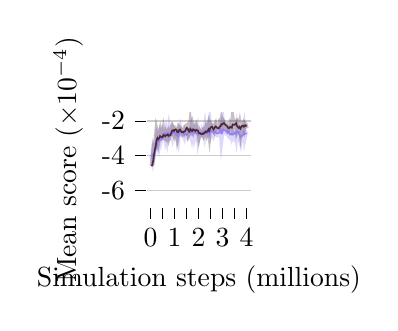
\begin{tikzpicture}

% \begin{axis}[
% axis background/.style={fill=white!82.7450980392157!black},
% axis line style={white},
% legend cell align={left},
% legend style={fill opacity=0.8, draw opacity=1, text opacity=1, at={(1,0.1)}, anchor=south east, draw=white!80!black},
% tick align=outside,
% tick pos=left,
% x grid style={white!69.0196078431373!black},
% xlabel={Timestep},
% xmajorgrids,
% xmin=-162030, xmax=4193970,
% xtick style={color=black},
% xtick={-500000,0,500000,1000000,1500000,2000000,2500000,3000000,3500000,4000000,4500000},
% xticklabels={-0.5M,0.0M,0.5M,1.0M,1.5M,2.0M,2.5M,3.0M,3.5M,4.0M,4.5M},
% y grid style={white!69.0196078431373!black},
% ylabel={Mean score},
% ymajorgrids,
% ymin=-10500, ymax=-1500,
% ytick style={color=black}
% ]
\definecolor{color0}{rgb}{0.83921568627451,0.152941176470588,0.156862745098039}
\definecolor{color1}{rgb}{0.12156862745098,0.966666666666667,0.205882352941177}
\definecolor{color2}{rgb}{0.580392156862745,0.503921568627451,0.941176470588235}
\definecolor{color3}{rgb}{0.290196078431372,0.166666666666667,0.23078431372549}

\begin{axis}[
    width=\figurewidth,
    height=\figureheight,
    axis background/.style={fill=white},
    axis line style={white},
    legend cell align={left},
    legend style={fill opacity=0.8, draw opacity=1, text opacity=1, at={(1,0.1)}, anchor=south east, draw=white!80!black},
    tick align=outside,
    tick pos=left,
    x grid style={white},
    xlabel={Simulation steps (millions)},
    xmajorgrids,
    xmin=-162030, 
    xmax=4193970,
    xtick style={color=black},
    xtick={-500000,0,500000,1000000,1500000,2000000,2500000,3000000,3500000,4000000,4500000},
    xticklabels={,0,,1,,2,,3,,4,},
    y grid style={white!80!black},
    ylabel={Mean score ($\times10^{-4}$)},
    ymajorgrids,
    ymin=-7000, 
    ymax=-1500,
    ytick={-10000,-8000,-6000,-4000,-2000},
    yticklabels={-10,-8,-6,-4,-2},
    ytick style={color=black},
    scaled y ticks = false,
    scaled x ticks = false
]
\addplot [ultra thick, color2, opacity=0.3, forget plot]
table {%
35970 -3943.32153320312
71970 -4174.580078125
107970 -3728.65161132812
143970 -3953.30126953125
179970 -3659.85571289062
215970 -3391.6826171875
251970 -3347.9912109375
287970 -2788.56665039062
323970 -2893.0927734375
359970 -3241.16381835938
395970 -2910.32641601562
431970 -3123.80419921875
467970 -2943.07006835938
503970 -2595.45190429688
539970 -2686.21508789062
575970 -2631.10302734375
611970 -2933.50463867188
647970 -2642.30078125
683970 -2948.55078125
719970 -2530.48217773438
755970 -3146.33666992188
791970 -2490.07275390625
827970 -2732.2109375
863970 -2625.02783203125
899970 -2831.88110351562
935970 -2437.00512695312
971970 -2533.31274414062
1007970 -2820.98120117188
1043970 -2841.92358398438
1079970 -2940.00048828125
1115970 -2779.38647460938
1151970 -3021.89013671875
1187970 -2528.52563476562
1223970 -2378.953125
1259970 -2689.07421875
1295970 -2643.09716796875
1331970 -2791.11328125
1367970 -2763.35400390625
1403970 -2900.74609375
1439970 -2666.15063476562
1475970 -2793.33081054688
1511970 -2871.4287109375
1547970 -2633.66723632812
1583970 -2541.12329101562
1619970 -2535.890625
1655970 -2718.03637695312
1691970 -2485.76245117188
1727970 -2800.32397460938
1763970 -2492.77392578125
1799970 -2408.18798828125
1835970 -2908.32861328125
1871970 -2738.55004882812
1907970 -2765.95776367188
1943970 -2547.8994140625
1979970 -3022.29272460938
2015970 -2732.92602539062
2051970 -2655.00927734375
2087970 -2729.59814453125
2123970 -2779.12231445312
2159970 -2524.3916015625
2195970 -2603.1005859375
2231970 -2813.43969726562
2267970 -2421.3720703125
2303970 -2800.23364257812
2339970 -2796.22192382812
2375970 -2712.96435546875
2411970 -2425.703125
2447970 -2961.40283203125
2483970 -2280.67700195312
2519970 -2642.11572265625
2555970 -2458.82348632812
2591970 -2652.8583984375
2627970 -2807.80004882812
2663970 -2694.13427734375
2699970 -2533.6142578125
2735970 -2763.36791992188
2771970 -2792.79150390625
2807970 -2699.0849609375
2843970 -2656.10693359375
2879970 -2505.2978515625
2915970 -2348.64916992188
2951970 -3020.15307617188
2987970 -2627.13134765625
3023970 -2186.30908203125
3059970 -2577.08227539062
3095970 -2578.4423828125
3131970 -2630.99340820312
3167970 -2732.62255859375
3203970 -2764.54809570312
3239970 -2262.10571289062
3275970 -2893.1865234375
3311970 -2937.20629882812
3347970 -2653.59985351562
3383970 -2871.04028320312
3419970 -2688.47192382812
3455970 -2817.1611328125
3491970 -2556.62084960938
3527970 -2582.46557617188
3563970 -2878.61938476562
3599970 -2385.15649414062
3635970 -2625.80517578125
3671970 -2745.83813476562
3707970 -2962.18383789062
3743970 -3155.08544921875
3779970 -2791.56689453125
3815970 -2851.30493164062
3851970 -2679.41772460938
3887970 -2399.96850585938
3923970 -2920.44653320312
3959970 -2689.23315429688
3995970 -2793.76904296875
};
\addplot [ultra thick, color3, opacity=0.3, forget plot]
table {%
35970 -4605.3837890625
71970 -4454.2998046875
107970 -3984.07348632812
143970 -3409.05395507812
179970 -3199.03662109375
215970 -3135.71752929688
251970 -2587.67065429688
287970 -2800.51147460938
323970 -3170.73950195312
359970 -2925.49658203125
395970 -2684.72119140625
431970 -2984.34594726562
467970 -2946.0244140625
503970 -2961.98681640625
539970 -2602.04736328125
575970 -2884.98046875
611970 -2955.76440429688
647970 -2727.80517578125
683970 -2846.62475585938
719970 -2714.01489257812
755970 -2963.49560546875
791970 -2817.5
827970 -2788.8271484375
863970 -2490.05200195312
899970 -2359.640625
935970 -2496.37329101562
971970 -2667.63916015625
1007970 -2407.30908203125
1043970 -2443.68579101562
1079970 -2523.6748046875
1115970 -2903.61303710938
1151970 -2638.89477539062
1187970 -2366.74877929688
1223970 -2425.63623046875
1259970 -2697.43798828125
1295970 -2733.15258789062
1331970 -2625.33032226562
1367970 -2692.90576171875
1403970 -2524.06958007812
1439970 -2583.76513671875
1475970 -2308.6572265625
1511970 -2271.65112304688
1547970 -2493.46630859375
1583970 -2780.18969726562
1619970 -2674.34594726562
1655970 -2218.89697265625
1691970 -2621.55541992188
1727970 -2676.0302734375
1763970 -2331.87548828125
1799970 -2515.83129882812
1835970 -2641.15161132812
1871970 -2619.27368164062
1907970 -2408.83666992188
1943970 -2584.90161132812
1979970 -2606.70166015625
2015970 -2888.70385742188
2051970 -2684.32177734375
2087970 -2815.11938476562
2123970 -2794.44165039062
2159970 -2681.7734375
2195970 -2780.7265625
2231970 -2600.76733398438
2267970 -2665.57788085938
2303970 -2482.95556640625
2339970 -2691.0771484375
2375970 -2523.96875
2411970 -2311.76342773438
2447970 -2703.81591796875
2483970 -2185.7958984375
2519970 -2267.03198242188
2555970 -2281.19311523438
2591970 -2546.48364257812
2627970 -2602.609375
2663970 -2275.27368164062
2699970 -2183.68115234375
2735970 -2378.84130859375
2771970 -2482.1904296875
2807970 -2461.61572265625
2843970 -2414.36450195312
2879970 -2183.81494140625
2915970 -2276.53784179688
2951970 -2002.92041015625
2987970 -2227.72998046875
3023970 -2023.66198730469
3059970 -2104.08715820312
3095970 -2279.24096679688
3131970 -2341.57666015625
3167970 -2285.05859375
3203970 -2459.90698242188
3239970 -2503.74438476562
3275970 -2439.59838867188
3311970 -2232.07690429688
3347970 -2346.38354492188
3383970 -2447.67065429688
3419970 -1922.345703125
3455970 -2237.4677734375
3491970 -2235.92724609375
3527970 -2089.3681640625
3563970 -2049.4765625
3599970 -2543.5546875
3635970 -2414.015625
3671970 -2492.52172851562
3707970 -2248.7939453125
3743970 -2592.58178710938
3779970 -2198.42553710938
3815970 -2160.37622070312
3851970 -2263.35400390625
3887970 -2422.40551757812
3923970 -2158.77465820312
3959970 -2220.48803710938
3995970 -2432.9677734375
};
\addplot [semithick, color2]
table {%
35970 -3943.32153320312
71970 -4035.82495117188
107970 -3912.95561523438
143970 -3929.09387695313
179970 -3821.39861132813
215970 -3649.51221367188
251970 -3528.90381257813
287970 -3232.76894770313
323970 -3096.89847799688
359970 -3154.60461414188
395970 -3056.89333489138
431970 -3083.65768062233
467970 -3027.42263571715
503970 -2854.63434314904
539970 -2787.26664104567
575970 -2724.8011955649
611970 -2808.28257280769
647970 -2741.88985618462
683970 -2824.55422621077
719970 -2706.92540682021
755970 -2882.68991206088
791970 -2725.64304879903
827970 -2728.27020427942
863970 -2686.97325538015
899970 -2744.93639463434
935970 -2621.76388756185
971970 -2586.38343019336
1007970 -2680.22253858477
1043970 -2744.90295674461
1079970 -2822.94196935927
1115970 -2805.51977145931
1151970 -2892.06791756309
1187970 -2746.6510044441
1223970 -2599.57185266646
1259970 -2635.37279909988
1295970 -2638.46254664743
1331970 -2699.52284048846
1367970 -2725.05530585557
1403970 -2795.33162101334
1439970 -2743.65922651426
1475970 -2763.5278601273
1511970 -2806.68820045138
1547970 -2737.47981480208
1583970 -2658.9372052875
1619970 -2609.7185731725
1655970 -2653.04569468475
1691970 -2586.1323972796
1727970 -2671.80902821151
1763970 -2600.19498723941
1799970 -2523.39218765614
1835970 -2677.36675790619
1871970 -2701.84007427496
1907970 -2727.48715003373
1943970 -2655.65205564524
1979970 -2802.30832323089
2015970 -2774.55540409478
2051970 -2726.73695339437
2087970 -2727.88142984912
2123970 -2748.37778369072
2159970 -2658.78331083943
2195970 -2636.51022087866
2231970 -2707.28201143345
2267970 -2592.91803498507
2303970 -2675.84427802229
2339970 -2723.99533634462
2375970 -2719.58294399427
2411970 -2602.03101639656
2447970 -2745.77974265044
2483970 -2559.73864637151
2519970 -2592.68947688541
2555970 -2539.14308066249
2591970 -2584.6292077725
2627970 -2673.89754419475
2663970 -2681.99223745435
2699970 -2622.64104559761
2735970 -2678.93179532732
2771970 -2724.47567875889
2807970 -2714.31939163033
2843970 -2691.0344084157
2879970 -2616.73978567442
2915970 -2509.5035393734
2951970 -2713.76335409279
2987970 -2679.11055151817
3023970 -2481.9899637234
3059970 -2520.02688839029
3095970 -2543.39308615918
3131970 -2578.43321497676
3167970 -2640.10895242355
3203970 -2689.88460973538
3239970 -2518.77305099748
3275970 -2668.53843997349
3311970 -2776.00558351534
3347970 -2727.04329151546
3383970 -2784.64208819052
3419970 -2746.17402244556
3455970 -2774.56886659234
3491970 -2687.38965979915
3527970 -2645.42002634824
3563970 -2738.69976971519
3599970 -2597.28245948537
3635970 -2608.69154600372
3671970 -2663.55018150848
3707970 -2783.00364406134
3743970 -2931.8363661243
3779970 -2875.72857748708
3815970 -2865.9591191485
3851970 -2791.34256133285
3887970 -2634.79293914346
3923970 -2749.05437676733
3959970 -2725.12588777915
3995970 -2752.58314985499
};
% \addlegendentry{Training}
\addplot [semithick, color3]
table {%
35970 -4605.3837890625
71970 -4544.9501953125
107970 -4320.59951171875
143970 -3955.9812890625
179970 -3653.203421875
215970 -3446.20906484375
251970 -3102.793700625
287970 -2981.88081021875
323970 -3057.4242869125
359970 -3004.65320496
395970 -2876.6803995385
431970 -2919.74661862935
467970 -2930.25773680261
503970 -2942.94936864407
539970 -2806.58856649894
575970 -2837.94532739936
611970 -2885.07295815837
647970 -2822.16584520752
683970 -2831.94940946826
719970 -2784.77560271221
755970 -2856.26360381482
791970 -2840.75816228889
827970 -2819.98575674834
863970 -2688.01225483025
899970 -2556.66360289815
935970 -2532.54747814514
971970 -2586.58415094958
1007970 -2514.87412338225
1043970 -2486.3987904356
1079970 -2501.30919613636
1115970 -2662.23073252557
1151970 -2652.89634967159
1187970 -2538.4373215217
1223970 -2493.31688510052
1259970 -2574.96532637281
1295970 -2638.24023097994
1331970 -2633.07626749421
1367970 -2657.00806518403
1403970 -2603.83267114167
1439970 -2595.8056573725
1475970 -2480.9462850485
1511970 -2397.22822024785
1547970 -2435.72345558621
1583970 -2573.50995225798
1619970 -2613.84435026104
1655970 -2455.86539921912
1691970 -2522.14140750022
1727970 -2583.69695387513
1763970 -2482.96836763758
1799970 -2496.1135401138
1835970 -2554.12876859953
1871970 -2580.18673381597
1907970 -2511.64670825833
1943970 -2540.94866948625
1979970 -2567.24986575425
2015970 -2695.8314624213
2051970 -2691.22758839028
2087970 -2740.78430694042
2123970 -2762.2472443205
2159970 -2730.0577215923
2195970 -2750.32525795538
2231970 -2690.50208836698
2267970 -2680.53240536394
2303970 -2601.50166978086
2339970 -2637.33186124352
2375970 -2591.98661674611
2411970 -2479.89734114142
2447970 -2569.46477187235
2483970 -2415.99722249841
2519970 -2356.4111264678
2555970 -2326.32392197443
2591970 -2414.38781021591
2627970 -2489.67643612954
2663970 -2403.91533433398
2699970 -2315.82166153789
2735970 -2341.02952036023
2771970 -2397.49388409114
2807970 -2423.14261951718
2843970 -2419.63137249156
2879970 -2325.30480005744
2915970 -2305.79801675321
2951970 -2184.64697411443
2987970 -2201.88017665616
3023970 -2130.59290091557
3059970 -2119.99060383059
3095970 -2183.6907490171
3131970 -2246.84511347276
3167970 -2262.13050558366
3203970 -2341.24109631894
3239970 -2406.24241169762
3275970 -2419.58480248732
3311970 -2344.58164321114
3347970 -2345.30240389544
3383970 -2386.24970405601
3419970 -2200.68810368361
3455970 -2215.39997158516
3491970 -2223.6108813886
3527970 -2169.91379445816
3563970 -2121.7389016749
3599970 -2290.46521600494
3635970 -2339.88537960296
3671970 -2400.93991916803
3707970 -2340.08152962582
3743970 -2441.08163261924
3779970 -2344.01919441529
3815970 -2270.56200493043
3851970 -2267.67880452076
3887970 -2329.5694897437
3923970 -2261.25155712747
3959970 -2244.94614912023
3995970 -2320.15479884714
};
% \addlegendentry{Evaluation}
\end{axis}

\end{tikzpicture}
}
        \caption{IV15}
        \label{fig:IV15}
    \end{subfigure}
    \begin{subfigure}[t]{0.24\textwidth}
        \centering
        \setlength{\figureheight}{0.8\textwidth}
        \setlength{\figurewidth}{\textwidth}
        \footnotesize{\input{fig_latex_v2/20200628T191601}}
        \caption{IV25}
        \label{fig:IV25}
    \end{subfigure}
    \begin{subfigure}[t]{0.24\textwidth}
        \centering
        \setlength{\figureheight}{0.8\textwidth}
        \setlength{\figurewidth}{\textwidth}
        \footnotesize{% This file was created by tikzplotlib v0.9.1.
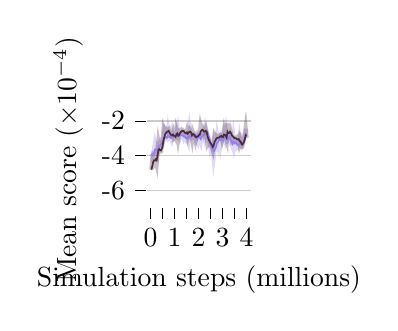
\begin{tikzpicture}

% \begin{axis}[
% axis background/.style={fill=white!82.7450980392157!black},
% axis line style={white},
% legend cell align={left},
% legend style={fill opacity=0.8, draw opacity=1, text opacity=1, at={(1,0.1)}, anchor=south east, draw=white!80!black},
% tick align=outside,
% tick pos=left,
% x grid style={white!69.0196078431373!black},
% xlabel={Timestep},
% xmajorgrids,
% xmin=-162030, xmax=4193970,
% xtick style={color=black},
% xtick={-500000,0,500000,1000000,1500000,2000000,2500000,3000000,3500000,4000000,4500000},
% xticklabels={-0.5M,0.0M,0.5M,1.0M,1.5M,2.0M,2.5M,3.0M,3.5M,4.0M,4.5M},
% y grid style={white!69.0196078431373!black},
% ylabel={Mean score},
% ymajorgrids,
% ymin=-10500, ymax=-1500,
% ytick style={color=black}
% ]
\definecolor{color0}{rgb}{0.83921568627451,0.152941176470588,0.156862745098039}
\definecolor{color1}{rgb}{0.12156862745098,0.966666666666667,0.205882352941177}
\definecolor{color2}{rgb}{0.580392156862745,0.503921568627451,0.941176470588235}
\definecolor{color3}{rgb}{0.290196078431372,0.166666666666667,0.23078431372549}

\begin{axis}[
    width=\figurewidth,
    height=\figureheight,
    axis background/.style={fill=white},
    axis line style={white},
    legend cell align={left},
    legend style={fill opacity=0.8, draw opacity=1, text opacity=1, at={(1,0.1)}, anchor=south east, draw=white!80!black},
    tick align=outside,
    tick pos=left,
    x grid style={white},
    xlabel={Simulation steps (millions)},
    xmajorgrids,
    xmin=-162030, 
    xmax=4193970,
    xtick style={color=black},
    xtick={-500000,0,500000,1000000,1500000,2000000,2500000,3000000,3500000,4000000,4500000},
    xticklabels={,0,,1,,2,,3,,4,},
    y grid style={white!80!black},
    ylabel={Mean score ($\times10^{-4}$)},
    ymajorgrids,
    ymin=-7000, 
    ymax=-1500,
    ytick={-10000,-8000,-6000,-4000,-2000},
    yticklabels={-10,-8,-6,-4,-2},
    ytick style={color=black},
    scaled y ticks = false,
    scaled x ticks = false
]
\addplot [ultra thick, color2, opacity=0.3, forget plot]
table {%
35970 -3915.8544921875
71970 -4076.91870117188
107970 -3958.078125
143970 -3671.94897460938
179970 -3355.51098632812
215970 -3607.49755859375
251970 -3644.24267578125
287970 -3826.96484375
323970 -3309.06860351562
359970 -3258.05908203125
395970 -3325.81323242188
431970 -3377.33447265625
467970 -3123.90673828125
503970 -3153.3564453125
539970 -3038.0302734375
575970 -2644.17138671875
611970 -2837.12280273438
647970 -3033.94897460938
683970 -3021.00854492188
719970 -2624.51098632812
755970 -2997.88110351562
791970 -2946.87475585938
827970 -2905.60766601562
863970 -3039.15869140625
899970 -2739.63916015625
935970 -3025.28588867188
971970 -2969.04760742188
1007970 -2917.43408203125
1043970 -2934.50732421875
1079970 -2682.57885742188
1115970 -2467.85620117188
1151970 -2943.46264648438
1187970 -2998.7744140625
1223970 -2730.64672851562
1259970 -2685.75952148438
1295970 -2888.66137695312
1331970 -2874.32739257812
1367970 -2992.83911132812
1403970 -2858.82006835938
1439970 -3011.85034179688
1475970 -3100.70874023438
1511970 -2986.54541015625
1547970 -2841.91088867188
1583970 -3059.84741210938
1619970 -2591.93872070312
1655970 -3020.82299804688
1691970 -2973.62841796875
1727970 -2743.37646484375
1763970 -2802.54614257812
1799970 -2891.52294921875
1835970 -2828.9521484375
1871970 -2773.7978515625
1907970 -3169.73217773438
1943970 -3252.18188476562
1979970 -2799.0302734375
2015970 -2780.54931640625
2051970 -3023.10302734375
2087970 -3181.5322265625
2123970 -2816.99047851562
2159970 -2768.22241210938
2195970 -2657.44506835938
2231970 -2868.66235351562
2267970 -2548.42797851562
2303970 -2854.86059570312
2339970 -2679.15942382812
2375970 -2774.43237304688
2411970 -3017.29541015625
2447970 -3111.79248046875
2483970 -3434.90991210938
2519970 -3817.65991210938
2555970 -3785.60107421875
2591970 -3503.9326171875
2627970 -4074.04541015625
2663970 -3682.9697265625
2699970 -3341.5400390625
2735970 -3359.8076171875
2771970 -2901.99975585938
2807970 -3213.32055664062
2843970 -2823.9873046875
2879970 -2853.09692382812
2915970 -3316.70629882812
2951970 -3010.1025390625
2987970 -3150.01293945312
3023970 -3139.49194335938
3059970 -2804.68115234375
3095970 -3014.3994140625
3131970 -2684.22827148438
3167970 -3178.53662109375
3203970 -3192.02587890625
3239970 -2881.2216796875
3275970 -2782.79614257812
3311970 -3111.74096679688
3347970 -3288.59716796875
3383970 -3362.5947265625
3419970 -3498.51171875
3455970 -3015.7138671875
3491970 -3419.44067382812
3527970 -3175.27661132812
3563970 -3274.55249023438
3599970 -3515.66528320312
3635970 -3464.11303710938
3671970 -3448.57666015625
3707970 -3036.11499023438
3743970 -3362.47485351562
3779970 -3444.77294921875
3815970 -3285.79638671875
3851970 -3248.38940429688
3887970 -2981.15502929688
3923970 -2779.26000976562
3959970 -2666.37670898438
3995970 -2454.32348632812
};
\addplot [ultra thick, color3, opacity=0.3, forget plot]
table {%
35970 -4813.912109375
71970 -4331.92041015625
107970 -4038.95361328125
143970 -4116.0400390625
179970 -4301.83056640625
215970 -4099.47216796875
251970 -4364.0009765625
287970 -3718.70361328125
323970 -3213.50366210938
359970 -3494.62475585938
395970 -3776.07763671875
431970 -3751.2060546875
467970 -3461.390625
503970 -3250.34936523438
539970 -2538.26684570312
575970 -2707.6572265625
611970 -2496.45849609375
647970 -2583.46215820312
683970 -2519.9716796875
719970 -2590.21069335938
755970 -2527.14965820312
791970 -2828.83984375
827970 -2888.07739257812
863970 -2903.79370117188
899970 -2862.34814453125
935970 -2695.0546875
971970 -2963.19921875
1007970 -2891.41259765625
1043970 -2988.04296875
1079970 -2501.94848632812
1115970 -2683.12060546875
1151970 -3053.14819335938
1187970 -2752.16943359375
1223970 -2543.63549804688
1259970 -2551.75463867188
1295970 -2500.20849609375
1331970 -2529.75463867188
1367970 -2596.32177734375
1403970 -2710.9775390625
1439970 -2787.81079101562
1475970 -2750.07177734375
1511970 -2569.25927734375
1547970 -2847.68725585938
1583970 -2612.88354492188
1619970 -2509.84838867188
1655970 -2609.15185546875
1691970 -2788.12817382812
1727970 -3051.61352539062
1763970 -2652.46215820312
1799970 -2788.2646484375
1835970 -2883.46240234375
1871970 -3119.67211914062
1907970 -2910.58837890625
1943970 -2862.87573242188
1979970 -2845.36596679688
2015970 -2705.49682617188
2051970 -2780.0751953125
2087970 -2300.19702148438
2123970 -2496.1826171875
2159970 -2428.32348632812
2195970 -2579.78491210938
2231970 -2753.93798828125
2267970 -2629.43212890625
2303970 -2476.4052734375
2339970 -2701.86010742188
2375970 -3329.9482421875
2411970 -3236.9140625
2447970 -3330.17602539062
2483970 -3387.93188476562
2519970 -3446.62768554688
2555970 -3500.95703125
2591970 -3659.83422851562
2627970 -3297.06689453125
2663970 -2894.64868164062
2699970 -3013.78662109375
2735970 -2869.55102539062
2771970 -2925.97998046875
2807970 -2953.6962890625
2843970 -2945.58129882812
2879970 -2869.30078125
2915970 -2809.2294921875
2951970 -2825.39624023438
2987970 -3075.74780273438
3023970 -2888.55786132812
3059970 -2565.46997070312
3095970 -2828.2548828125
3131970 -2928.26293945312
3167970 -3105.0771484375
3203970 -2123.70043945312
3239970 -2850.58569335938
3275970 -2660.31127929688
3311970 -2531.015625
3347970 -2790.98120117188
3383970 -3049.35571289062
3419970 -2950.01928710938
3455970 -2991.62573242188
3491970 -3083.21508789062
3527970 -3022.90795898438
3563970 -2981.74951171875
3599970 -3155.03491210938
3635970 -3100.83642578125
3671970 -2986.91137695312
3707970 -3333.6220703125
3743970 -3174.84375
3779970 -3485.25317382812
3815970 -3480.28686523438
3851970 -3223.09887695312
3887970 -3064.23999023438
3923970 -2849.73706054688
3959970 -2460.72973632812
3995970 -2980.91284179688
};
\addplot [semithick, color2]
table {%
35970 -3915.8544921875
71970 -3980.28017578125
107970 -3971.39935546875
143970 -3851.619203125
179970 -3653.17591640625
215970 -3634.90457328125
251970 -3638.63981428125
287970 -3713.96982606875
323970 -3552.0093370475
359970 -3434.429235041
395970 -3390.98283399335
431970 -3385.52348945851
467970 -3280.87678898761
503970 -3229.86865151756
539970 -3153.13330028554
575970 -2949.54853485882
611970 -2904.57824200904
647970 -2956.32653504918
683970 -2982.19933899826
719970 -2839.1239979302
755970 -2902.62684016437
791970 -2920.32600644237
827970 -2914.43867027167
863970 -2964.3266787255
899970 -2874.4516712978
935970 -2934.78535824743
971970 -2948.49025791721
1007970 -2936.06778756283
1043970 -2935.44360222519
1079970 -2834.29770430387
1115970 -2687.72110305107
1151970 -2790.01772042439
1187970 -2873.52039787964
1223970 -2816.37093013403
1259970 -2764.12636667417
1295970 -2813.94037078575
1331970 -2838.0951795027
1367970 -2899.99275223287
1403970 -2883.52367868347
1439970 -2934.85434392883
1475970 -3001.19610245105
1511970 -2995.33582553313
1547970 -2933.96585078863
1583970 -2984.31847531693
1619970 -2827.36657347141
1655970 -2904.74914330159
1691970 -2932.30085316846
1727970 -2856.73109783857
1763970 -2835.05711573439
1799970 -2857.64344912814
1835970 -2846.16692885188
1871970 -2817.21929793613
1907970 -2958.22444985543
1943970 -3075.80742381951
1979970 -2965.0965636667
2015970 -2891.27766476252
2051970 -2944.00780979501
2087970 -3039.01757650201
2123970 -2950.20673730746
2159970 -2877.41300722822
2195970 -2789.42583168068
2231970 -2821.12044041466
2267970 -2712.04345565505
2303970 -2769.17031167428
2339970 -2733.16595653582
2375970 -2749.67252314024
2411970 -2856.72167794664
2447970 -2958.74999895549
2483970 -3149.21396421704
2519970 -3416.59234337397
2555970 -3564.19583571189
2591970 -3540.09054830213
2627970 -3753.67249304378
2663970 -3725.39138645127
2699970 -3571.85084749576
2735970 -3487.03355537246
2771970 -3253.02003556722
2807970 -3237.14024399658
2843970 -3071.87906827295
2879970 -2984.36621049502
2915970 -3117.30224582826
2951970 -3074.42236312196
2987970 -3104.65859365442
3023970 -3118.5919335364
3059970 -2993.02762105934
3095970 -3001.57633826061
3131970 -2874.63711155011
3167970 -2996.19691536757
3203970 -3074.52850078304
3239970 -2997.20577234482
3275970 -2911.44192043814
3311970 -2991.56153898164
3347970 -3110.37579057648
3383970 -3211.26336497089
3419970 -3326.16270648253
3455970 -3201.98317076452
3491970 -3288.96617198996
3527970 -3243.49034772523
3563970 -3255.91520472889
3599970 -3359.81523611858
3635970 -3401.5343565149
3671970 -3420.35127797144
3707970 -3266.65676287661
3743970 -3304.98399913222
3779970 -3360.89957916683
3815970 -3330.8583021876
3851970 -3297.87074303131
3887970 -3171.18445753754
3923970 -3014.41467842877
3959970 -2875.19949065101
3995970 -2706.84908892186
};
% \addlegendentry{Training}
\addplot [semithick, color3]
table {%
35970 -4813.912109375
71970 -4621.1154296875
107970 -4388.250703125
143970 -4279.3664375
179970 -4288.3520890625
215970 -4212.800120625
251970 -4273.280463
287970 -4051.4497231125
323970 -3716.27129871125
359970 -3627.6126815705
395970 -3686.9986636298
431970 -3712.68162005288
467970 -3612.16522203173
503970 -3467.43887931279
539970 -3095.77006586892
575970 -2940.52493014635
611970 -2762.89835652531
647970 -2691.12387719644
683970 -2622.66299819286
719970 -2609.68207625947
755970 -2576.66910903693
791970 -2677.53740292216
827970 -2761.75339878454
863970 -2818.56951973948
899970 -2836.08096965619
935970 -2779.67045679371
971970 -2853.08196157623
1007970 -2868.41421600824
1043970 -2916.26571710494
1079970 -2750.53882479422
1115970 -2723.57153706403
1151970 -2855.40219958217
1187970 -2814.1090931868
1223970 -2705.91965513083
1259970 -2644.25364854725
1295970 -2586.63558756585
1331970 -2563.88320800826
1367970 -2576.85863574246
1403970 -2630.50619707047
1439970 -2693.42803464853
1475970 -2716.08553172662
1511970 -2657.35502997347
1547970 -2733.48792032783
1583970 -2685.24617016545
1619970 -2615.08705756802
1655970 -2612.71297672831
1691970 -2682.87905556824
1727970 -2830.37284349719
1763970 -2759.20856937957
1799970 -2770.83100100274
1835970 -2815.88356153914
1871970 -2937.39898457974
1907970 -2926.67474231034
1943970 -2901.15513835495
1979970 -2878.83946973172
2015970 -2809.50241230778
2051970 -2797.73152550967
2087970 -2598.71772389955
2123970 -2557.70368121473
2159970 -2505.95160326009
2195970 -2535.4849267998
2231970 -2622.86615139238
2267970 -2625.49254239793
2303970 -2565.85763481376
2339970 -2620.258623857
2375970 -2904.1344711892
2411970 -3037.24630771352
2447970 -3154.41819478436
2483970 -3247.82367077687
2519970 -3327.34527668487
2555970 -3396.78997851092
2591970 -3502.0076785128
2627970 -3420.03136492018
2663970 -3209.87829160836
2699970 -3131.44162340252
2735970 -3026.68538419776
2771970 -2986.40322270616
2807970 -2973.32044924869
2843970 -2962.22478908047
2879970 -2925.05518594828
2915970 -2878.72490844397
2951970 -2857.39344116013
2987970 -2944.73518578983
3023970 -2922.26425600515
3059970 -2779.54654188434
3095970 -2799.0298782556
3131970 -2850.72310273461
3167970 -2952.46472101577
3203970 -2620.95900839071
3239970 -2712.80968237818
3275970 -2691.81032114566
3311970 -2627.49244268739
3347970 -2692.88794608119
3383970 -2835.47505280496
3419970 -2881.29274652673
3455970 -2925.42594088479
3491970 -2988.54159968712
3527970 -3002.28814340602
3563970 -2994.07269073111
3599970 -3058.45757928242
3635970 -3075.40911788195
3671970 -3040.01002151042
3707970 -3157.45484103125
3743970 -3164.41040461875
3779970 -3292.7475123025
3815970 -3367.76325347525
3851970 -3309.8975028664
3887970 -3211.63449781359
3923970 -3066.8755229069
3959970 -2824.41720827539
3995970 -2887.01546168399
};
% \addlegendentry{Evaluation}
\end{axis}

\end{tikzpicture}
}
        \caption{OF5}
        \label{fig:OF5}
    \end{subfigure}
    \begin{subfigure}[t]{0.24\textwidth}
        \centering
        \setlength{\figureheight}{0.8\textwidth}
        \setlength{\figurewidth}{\textwidth}
        \footnotesize{% This file was created by tikzplotlib v0.9.1.
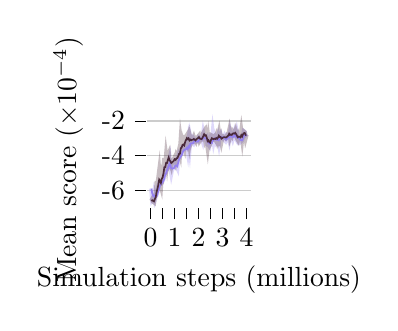
\begin{tikzpicture}

% \begin{axis}[
% axis background/.style={fill=white!82.7450980392157!black},
% axis line style={white},
% legend cell align={left},
% legend style={fill opacity=0.8, draw opacity=1, text opacity=1, at={(1,0.1)}, anchor=south east, draw=white!80!black},
% tick align=outside,
% tick pos=left,
% x grid style={white!69.0196078431373!black},
% xlabel={Simulation steps},
% xmajorgrids,
% xmin=-162030, xmax=4193970,
% xtick style={color=black},
% xtick={-500000,0,500000,1000000,1500000,2000000,2500000,3000000,3500000,4000000,4500000},
% xticklabels={-0.5M,0.0M,0.5M,1.0M,1.5M,2.0M,2.5M,3.0M,3.5M,4.0M,4.5M},
% y grid style={white!69.0196078431373!black},
% ylabel={Mean score},
% ymajorgrids,
% ymin=-7000, ymax=-1500,
% ytick style={color=black}
% ]
\definecolor{color0}{rgb}{0.83921568627451,0.152941176470588,0.156862745098039}
\definecolor{color1}{rgb}{0.12156862745098,0.966666666666667,0.205882352941177}
\definecolor{color2}{rgb}{0.580392156862745,0.503921568627451,0.941176470588235}
\definecolor{color3}{rgb}{0.290196078431372,0.166666666666667,0.23078431372549}

\begin{axis}[
    width=\figurewidth,
    height=\figureheight,
    axis background/.style={fill=white},
    axis line style={white},
    legend cell align={left},
    legend style={fill opacity=0.8, draw opacity=1, text opacity=1, at={(1,0.1)}, anchor=south east, draw=white!80!black},
    tick align=outside,
    tick pos=left,
    x grid style={white},
    xlabel={Simulation steps (millions)},
    xmajorgrids,
    xmin=-162030, 
    xmax=4193970,
    xtick style={color=black},
    xtick={-500000,0,500000,1000000,1500000,2000000,2500000,3000000,3500000,4000000,4500000},
    xticklabels={,0,,1,,2,,3,,4,},
    y grid style={white!80!black},
    ylabel={Mean score ($\times10^{-4}$)},
    ymajorgrids,
    ymin=-7000, 
    ymax=-1500,
    ytick={-10000,-8000,-6000,-4000,-2000},
    yticklabels={-10,-8,-6,-4,-2},
    ytick style={color=black},
    scaled y ticks = false,
    scaled x ticks = false
]
\addplot [ultra thick, color2, opacity=0.3, forget plot]
table {%
35970 -5913.4248046875
71970 -6612.62451171875
107970 -6560.20947265625
143970 -6252.6220703125
179970 -6524.3447265625
215970 -6370.4326171875
251970 -6256.2900390625
287970 -6073.8330078125
323970 -5802.22314453125
359970 -5631.0859375
395970 -5497.71435546875
431970 -5477.76513671875
467970 -5537.65576171875
503970 -5439.17919921875
539970 -5354.07958984375
575970 -5101.16650390625
611970 -4811.8076171875
647970 -4854.8369140625
683970 -4609.49853515625
719970 -4580.0498046875
755970 -4414.71240234375
791970 -4211.41357421875
827970 -4737.1005859375
863970 -5011.326171875
899970 -4764.38037109375
935970 -4731.58837890625
971970 -4720.0751953125
1007970 -4441.76806640625
1043970 -4519.2509765625
1079970 -4582.1083984375
1115970 -4693.45361328125
1151970 -4098.52490234375
1187970 -3924.73803710938
1223970 -4002.23803710938
1259970 -3931.80908203125
1295970 -3898.1591796875
1331970 -3561.73120117188
1367970 -3588.7607421875
1403970 -3591.3017578125
1439970 -3593.28076171875
1475970 -3633.51782226562
1511970 -3423.96362304688
1547970 -3726.09765625
1583970 -3240.6884765625
1619970 -3593.21166992188
1655970 -3005.28686523438
1691970 -3263.4541015625
1727970 -3288.17651367188
1763970 -3316.23583984375
1799970 -3041.0537109375
1835970 -3108.55029296875
1871970 -3201.77001953125
1907970 -3199.33276367188
1943970 -3187.41870117188
1979970 -3186.95385742188
2015970 -2972.97534179688
2051970 -3007.4638671875
2087970 -2977.42041015625
2123970 -2972.68505859375
2159970 -3122.46923828125
2195970 -2744.6806640625
2231970 -2987.82275390625
2267970 -3046.50244140625
2303970 -3076.34838867188
2339970 -2997.95434570312
2375970 -3344.91552734375
2411970 -3338.61254882812
2447970 -3418.57641601562
2483970 -3171.68090820312
2519970 -3332.3095703125
2555970 -3274.57080078125
2591970 -2744.90063476562
2627970 -3129.59838867188
2663970 -2871.13671875
2699970 -3025.42358398438
2735970 -3200.48828125
2771970 -3111.06811523438
2807970 -2933.73510742188
2843970 -3219.30419921875
2879970 -2852.0009765625
2915970 -2770.75732421875
2951970 -2958.61352539062
2987970 -2953.34716796875
3023970 -3009.40698242188
3059970 -2913.00659179688
3095970 -3113.16333007812
3131970 -3166.88452148438
3167970 -3085.89624023438
3203970 -2802.0927734375
3239970 -2795.37841796875
3275970 -3024.24926757812
3311970 -2709.1083984375
3347970 -2963.13647460938
3383970 -2874.77416992188
3419970 -3025.48999023438
3455970 -2847.39086914062
3491970 -2677.82592773438
3527970 -2939.99438476562
3563970 -3026.6064453125
3599970 -2714.23583984375
3635970 -2956.1728515625
3671970 -3137.74438476562
3707970 -3073.24682617188
3743970 -3199.78442382812
3779970 -3155.69921875
3815970 -3105.81982421875
3851970 -2871.8466796875
3887970 -2608.95703125
3923970 -2648.74194335938
3959970 -2881.42407226562
3995970 -2934.59008789062
};
\addplot [ultra thick, color3, opacity=0.3, forget plot]
table {%
35970 -6625.818359375
71970 -6527.32861328125
107970 -6661.0634765625
143970 -6700.21044921875
179970 -6299.39892578125
215970 -6278.72216796875
251970 -5641.09375
287970 -5659.3154296875
323970 -5332.92138671875
359970 -4941.28857421875
395970 -5579.4755859375
431970 -5763.27001953125
467970 -4992.27294921875
503970 -5126.96533203125
539970 -4690.49560546875
575970 -4147.84716796875
611970 -4657.21826171875
647970 -4054.84326171875
683970 -4441.57666015625
719970 -3999.38232421875
755970 -3885.93310546875
791970 -4513.3828125
827970 -4418.93896484375
863970 -4587.9375
899970 -4321.91650390625
935970 -4284.76220703125
971970 -4200.990234375
1007970 -4100.91064453125
1043970 -4300.9521484375
1079970 -4025.72924804688
1115970 -4127.48779296875
1151970 -3901.67114257812
1187970 -3690.72021484375
1223970 -3882.24682617188
1259970 -3107.34252929688
1295970 -3457.18969726562
1331970 -3153.13037109375
1367970 -3327.98681640625
1403970 -3499.34692382812
1439970 -2922.75341796875
1475970 -2915.46435546875
1511970 -2836.1640625
1547970 -3141.78686523438
1583970 -2929.51831054688
1619970 -3311.26293945312
1655970 -2987.1796875
1691970 -3185.28247070312
1727970 -3038.93920898438
1763970 -3095.25512695312
1799970 -2961.84350585938
1835970 -3129.59643554688
1871970 -3195.27221679688
1907970 -2959.7734375
1943970 -2964.23022460938
1979970 -2916.59375
2015970 -2854.4345703125
2051970 -3146.5546875
2087970 -3072.0888671875
2123970 -3072.4296875
2159970 -2887.51171875
2195970 -2704.45751953125
2231970 -2618.33349609375
2267970 -2961.9873046875
2303970 -2781.89184570312
2339970 -3133.41821289062
2375970 -3489.41845703125
2411970 -3041.49731445312
2447970 -3409.41845703125
2483970 -3300.56298828125
2519970 -2829.58325195312
2555970 -2858.45141601562
2591970 -3081.4765625
2627970 -3086.08178710938
2663970 -2976.14404296875
2699970 -3066.64331054688
2735970 -2896.92309570312
2771970 -3094.90966796875
2807970 -2881.3447265625
2843970 -2671.57470703125
2879970 -3045.76708984375
2915970 -2908.80200195312
2951970 -3180.97143554688
2987970 -2943.90258789062
3023970 -2893.21362304688
3059970 -2908.25463867188
3095970 -2936.43505859375
3131970 -2992.7998046875
3167970 -2915.62622070312
3203970 -2789.51049804688
3239970 -2796.99584960938
3275970 -2568.59619140625
3311970 -2912.1298828125
3347970 -2752.18969726562
3383970 -2835.23657226562
3419970 -2616.48388671875
3455970 -2687.08666992188
3491970 -2757.44360351562
3527970 -2608.81762695312
3563970 -2874.1953125
3599970 -3000.22802734375
3635970 -3086.31640625
3671970 -2827.85571289062
3707970 -2940.609375
3743970 -2994.15649414062
3779970 -2621.73681640625
3815970 -3005.3017578125
3851970 -2574.92431640625
3887970 -2619.31811523438
3923970 -2670.2734375
3959970 -2977.56713867188
3995970 -2788.70947265625
};
\addplot [semithick, color2]
table {%
35970 -5913.4248046875
71970 -6193.1046875
107970 -6339.9466015625
143970 -6305.0167890625
179970 -6392.7479640625
215970 -6383.8218253125
251970 -6332.8091108125
287970 -6229.2186696125
323970 -6058.42045958
359970 -5887.486650748
395970 -5731.5777326363
431970 -5630.05269426928
467970 -5593.09392124907
503970 -5531.52803243694
539970 -5460.54865539967
575970 -5316.7957948023
611970 -5114.80052375638
647970 -5010.81507987883
683970 -4850.2884619898
719970 -4742.19299906888
755970 -4611.20076037883
791970 -4451.2858859148
827970 -4565.61176592388
863970 -4743.89752830433
899970 -4752.0906654201
935970 -4743.88975081456
971970 -4734.36392861373
1007970 -4617.32558373074
1043970 -4578.09574086344
1079970 -4579.70080389307
1115970 -4625.20192764834
1151970 -4414.5311175265
1187970 -4218.61388535965
1223970 -4132.06354605954
1259970 -4051.96176044823
1295970 -3990.44072814393
1331970 -3818.95691735511
1367970 -3726.87844728807
1403970 -3672.64777149784
1439970 -3640.9009675862
1475970 -3637.94770945797
1511970 -3552.35407489353
1547970 -3621.85150743612
1583970 -3469.38629508667
1619970 -3518.91644502075
1655970 -3313.4646131062
1691970 -3293.46040848872
1727970 -3291.34685056198
1763970 -3301.30244627469
1799970 -3197.20295213981
1835970 -3161.74188847139
1871970 -3177.75314089533
1907970 -3186.38499000595
1943970 -3186.79847447232
1979970 -3186.86062765214
2015970 -3101.30651331003
2051970 -3063.76945486102
2087970 -3029.22983697911
2123970 -3006.61192562497
2159970 -3052.95485068748
2195970 -2929.64517603749
2231970 -2952.91620718499
2267970 -2990.3507008735
2303970 -3024.74977599285
2339970 -3014.03160387696
2375970 -3146.38517326368
2411970 -3223.27612348946
2447970 -3301.39624049992
2483970 -3249.5101075812
2519970 -3282.62989267372
2555970 -3279.40625591673
2591970 -3065.60400745629
2627970 -3091.20175994252
2663970 -3003.17574346551
2699970 -3012.07487967306
2735970 -3087.44024030383
2771970 -3096.89139027605
2807970 -3031.62887713438
2843970 -3106.69900596813
2879970 -3004.81979420588
2915970 -2911.19480621103
2951970 -2930.16229388287
2987970 -2939.43624351722
3023970 -2967.42453907908
3059970 -2945.6573601662
3095970 -3012.65974813097
3131970 -3074.34965747233
3167970 -3078.96829057715
3203970 -2968.21808372129
3239970 -2899.08221742027
3275970 -2949.14903748341
3311970 -2853.13278186505
3347970 -2897.13425896278
3383970 -2888.19022334642
3419970 -2943.1101301016
3455970 -2904.82242571721
3491970 -2814.02382652408
3527970 -2864.4120498207
3563970 -2929.28980801742
3599970 -2843.26822074795
3635970 -2888.43007307377
3671970 -2988.15579775051
3707970 -3022.19220911906
3743970 -3093.22909500268
3779970 -3118.21714450161
3815970 -3113.25821638847
3851970 -3016.69360170808
3887970 -2853.59897352485
3923970 -2771.65616145866
3959970 -2815.56332578145
3995970 -2863.17403062512
};
%\addlegendentry{Training}
\addplot [semithick, color3]
table {%
35970 -6625.818359375
71970 -6586.4224609375
107970 -6616.2788671875
143970 -6649.8515
179970 -6509.6704703125
215970 -6417.291149375
251970 -6106.812189625
287970 -5927.81348565
323970 -5689.8566460775
359970 -5390.429417334
395970 -5466.0478847754
431970 -5584.93673867774
467970 -5347.87122289414
503970 -5259.50886654899
539970 -5031.90356211689
575970 -4678.28100445763
611970 -4669.85590736208
647970 -4423.85084910475
683970 -4430.94117352535
719970 -4258.31763380271
755970 -4109.36382246913
791970 -4270.97141848148
827970 -4330.15843702639
863970 -4433.27006221583
899970 -4388.728638892
935970 -4347.1420661477
971970 -4288.68133343862
1007970 -4213.57305787567
1043970 -4248.5246941004
1079970 -4159.40651567899
1115970 -4146.63902659489
1151970 -4048.65187298819
1187970 -3905.47920973041
1223970 -3896.186256307
1259970 -3580.64876550295
1295970 -3531.26513820802
1331970 -3380.01123136231
1367970 -3359.20146537989
1403970 -3415.25964875918
1439970 -3218.25715644301
1475970 -3097.14003605331
1511970 -2992.74964663198
1547970 -3052.36453407294
1583970 -3003.22604466251
1619970 -3126.44080257876
1655970 -3070.73635654726
1691970 -3116.5548022096
1727970 -3085.50856491951
1763970 -3089.40718973296
1799970 -3038.38171618352
1835970 -3074.86760392886
1871970 -3123.02944907607
1907970 -3057.72704444564
1943970 -3020.32831651113
1979970 -2978.83448990668
2015970 -2929.07452206901
2051970 -3016.06658824141
2087970 -3038.47549981984
2123970 -3052.05717489191
2159970 -2986.23899243514
2195970 -2873.52640327359
2231970 -2771.44924040165
2267970 -2847.66446611599
2303970 -2821.35541795084
2339970 -2946.18053592676
2375970 -3163.47570436855
2411970 -3114.68434840238
2447970 -3232.57799185393
2483970 -3259.77199042486
2519970 -3087.69649503616
2555970 -2995.99846342795
2591970 -3030.18970305677
2627970 -3052.54653667781
2663970 -3021.98553919419
2699970 -3039.84864773526
2735970 -2982.67842692241
2771970 -3027.57092334094
2807970 -2969.08044462957
2843970 -2850.07814959024
2879970 -2928.35372569164
2915970 -2920.53303619624
2951970 -3024.70839593649
2987970 -2992.38607271814
3023970 -2952.71709284964
3059970 -2934.93211117853
3095970 -2935.53329014462
3131970 -2958.43989596177
3167970 -2941.31442585831
3203970 -2880.59285473374
3239970 -2847.15405268399
3275970 -2735.7309081729
3311970 -2806.29049802874
3347970 -2784.65017772349
3383970 -2804.88473554035
3419970 -2729.52439601171
3455970 -2712.54930557577
3491970 -2730.50702475171
3527970 -2681.83126563228
3563970 -2758.77688437937
3599970 -2855.35734156512
3635970 -2947.74096743907
3671970 -2899.78686561969
3707970 -2916.11586937182
3743970 -2947.33211927934
3779970 -2817.0939981301
3815970 -2892.37710200306
3851970 -2765.39598776434
3887970 -2706.96483875235
3923970 -2692.28827825141
3959970 -2806.3998224196
3995970 -2799.32368251426
};
%\addlegendentry{Evaluation}
\end{axis}

\end{tikzpicture}
}
        \caption{OF15}
        \label{fig:OF15}
    \end{subfigure}
    \begin{subfigure}[t]{0.24\textwidth}
        \centering
        \setlength{\figureheight}{0.8\textwidth}
        \setlength{\figurewidth}{\textwidth}
        \footnotesize{% This file was created by tikzplotlib v0.9.1.
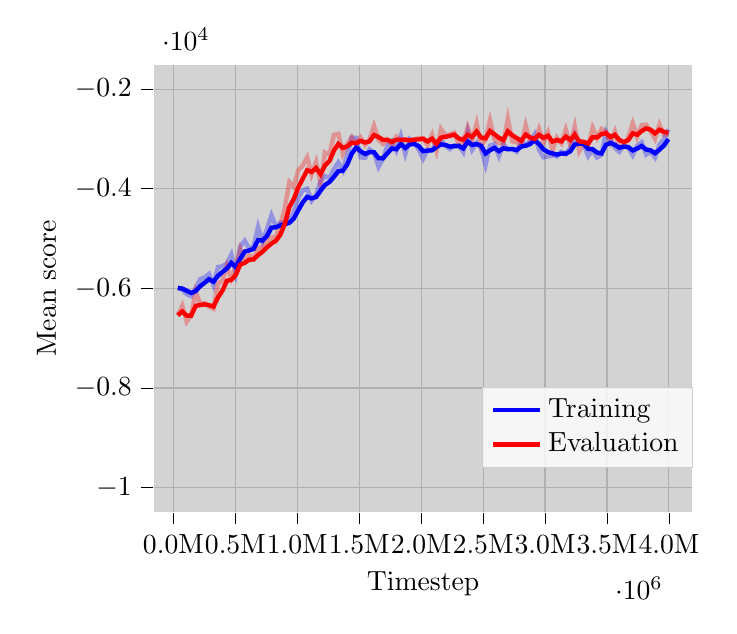
\begin{tikzpicture}

\begin{axis}[
axis background/.style={fill=white!82.7450980392157!black},
axis line style={white},
legend cell align={left},
legend style={fill opacity=0.8, draw opacity=1, text opacity=1, at={(1,0.1)}, anchor=south east, draw=white!80!black},
tick align=outside,
tick pos=left,
x grid style={white!69.0196078431373!black},
xlabel={Timestep},
xmajorgrids,
xmin=-162030, xmax=4193970,
xtick style={color=black},
xtick={-500000,0,500000,1000000,1500000,2000000,2500000,3000000,3500000,4000000,4500000},
xticklabels={-0.5M,0.0M,0.5M,1.0M,1.5M,2.0M,2.5M,3.0M,3.5M,4.0M,4.5M},
y grid style={white!69.0196078431373!black},
ylabel={Mean score},
ymajorgrids,
ymin=-10500, ymax=-1500,
ytick style={color=black}
]
\addplot [ultra thick, blue, opacity=0.3, forget plot]
table {%
35970 -5991.072265625
71970 -6026.36865234375
107970 -6115.931640625
143970 -6155.86865234375
179970 -6000.7548828125
215970 -5814.5498046875
251970 -5781.6865234375
287970 -5710.0458984375
323970 -5938.85205078125
359970 -5573.5205078125
395970 -5556.4765625
431970 -5500.55419921875
467970 -5322.4072265625
503970 -5695.19580078125
539970 -5158.52197265625
575970 -5043.44091796875
611970 -5204.25537109375
647970 -5158.6015625
683970 -4766.82666015625
719970 -5056.22216796875
755970 -4808.16552734375
791970 -4533.33642578125
827970 -4759.8349609375
863970 -4677.61669921875
899970 -4679.38232421875
935970 -4639.49267578125
971970 -4474.11083984375
1007970 -4185.14306640625
1043970 -4037.4189453125
1079970 -3998.4404296875
1115970 -4238.029296875
1151970 -4123.99755859375
1187970 -3848.3369140625
1223970 -3751.53735351562
1259970 -3778.37451171875
1295970 -3608.55810546875
1331970 -3472.13012695312
1367970 -3628.73510742188
1403970 -3318.55615234375
1439970 -2972.48095703125
1475970 -2980.09838867188
1511970 -3371.88525390625
1547970 -3380.54248046875
1583970 -3210.69995117188
1619970 -3273.17333984375
1655970 -3560.6640625
1691970 -3396.5908203125
1727970 -3134.35913085938
1763970 -3044.49829101562
1799970 -3232.84643554688
1835970 -2945.35864257812
1871970 -3301.40112304688
1907970 -3004.76538085938
1943970 -3084.72998046875
1979970 -3207.49682617188
2015970 -3399.99877929688
2051970 -3217.84692382812
2087970 -3219.58374023438
2123970 -3069.91552734375
2159970 -3024.08349609375
2195970 -3141.76489257812
2231970 -3203.7578125
2267970 -3130.6650390625
2303970 -3134.546875
2339970 -3264.82836914062
2375970 -2853.35766601562
2411970 -3217.47778320312
2447970 -3078.50708007812
2483970 -3188.8505859375
2519970 -3521.70263671875
2555970 -3134.86328125
2591970 -3105.87548828125
2627970 -3345.1953125
2663970 -3106.23754882812
2699970 -3219.66723632812
2735970 -3205.03515625
2771970 -3254.62524414062
2807970 -3049.625
2843970 -3110.08081054688
2879970 -3055.8671875
2915970 -2907.30908203125
2951970 -3220.22924804688
2987970 -3367.0732421875
3023970 -3350.43872070312
3059970 -3330.2509765625
3095970 -3351.41625976562
3131970 -3258.39794921875
3167970 -3302.32055664062
3203970 -3176.22143554688
3239970 -2907.9189453125
3275970 -3068.76782226562
3311970 -3107.29931640625
3347970 -3345.75634765625
3383970 -3222.66333007812
3419970 -3372.24267578125
3455970 -3318.28295898438
3491970 -2861.62231445312
3527970 -3025.76733398438
3563970 -3173.83764648438
3599970 -3261.77587890625
3635970 -3124.29907226562
3671970 -3179.08837890625
3707970 -3328.66040039062
3743970 -3136.57788085938
3779970 -3067.26000976562
3815970 -3314.11254882812
3851970 -3256.10400390625
3887970 -3373.60229492188
3923970 -3112.36938476562
3959970 -3006.03833007812
3995970 -2810.81811523438
};
\addplot [ultra thick, red, opacity=0.3, forget plot]
table {%
35970 -6541.26318359375
71970 -6349.5830078125
107970 -6670.09814453125
143970 -6546.38232421875
179970 -6062.53271484375
215970 -6304.876953125
251970 -6301.37744140625
287970 -6364.0703125
323970 -6407.837890625
359970 -5907.14501953125
395970 -5842.87451171875
431970 -5549.50634765625
467970 -5804.6123046875
503970 -5579.427734375
539970 -5209.86376953125
575970 -5434.21337890625
611970 -5334.58642578125
647970 -5406.849609375
683970 -5203.52392578125
719970 -5162.02978515625
755970 -5045.84619140625
791970 -4982.9169921875
827970 -4962.86865234375
863970 -4733.11181640625
899970 -4382.57763671875
935970 -3863.90869140625
971970 -3961.46826171875
1007970 -3630.8427734375
1043970 -3536.77856445312
1079970 -3370.17504882812
1115970 -3714.7041015625
1151970 -3463.68701171875
1187970 -3892.38061523438
1223970 -3271.84497070312
1259970 -3314.30688476562
1295970 -2917.70654296875
1331970 -2898.16186523438
1367970 -3299.39624023438
1403970 -3102.71508789062
1439970 -2963.78759765625
1475970 -3104.02734375
1511970 -2970.3154296875
1547970 -3120.30151367188
1583970 -3010.75708007812
1619970 -2738.55639648438
1655970 -3020.79272460938
1691970 -3100.99194335938
1727970 -3018.46142578125
1763970 -3119.69018554688
1799970 -2957.22192382812
1835970 -3026.34033203125
1871970 -3006.37255859375
1907970 -3045.85229492188
1943970 -3002.47875976562
1979970 -2993.80297851562
2015970 -2985.12548828125
2051970 -3124.29345703125
2087970 -2918.98461914062
2123970 -3237.85961914062
2159970 -2799.65991210938
2195970 -2930.14379882812
2231970 -2909.06469726562
2267970 -2878.63916015625
2303970 -3103.95361328125
2339970 -3059.97436523438
2375970 -2765.89721679688
2411970 -3020.46240234375
2447970 -2691.98559570312
2483970 -3150.41845703125
2519970 -3014.0517578125
2555970 -2624.88623046875
2591970 -3007.69677734375
2627970 -3079.32006835938
2663970 -3090.07055664062
2699970 -2592.1484375
2735970 -3046.1875
2771970 -3064.06005859375
2807970 -3123.7607421875
2843970 -2725.47924804688
2879970 -3054.6455078125
2915970 -3049.29296875
2951970 -2798.31176757812
2987970 -3067.80004882812
3023970 -2869.73388671875
3059970 -3229.2197265625
3095970 -2976.18579101562
3131970 -3087.68872070312
3167970 -2810.76098632812
3203970 -3128.67626953125
3239970 -2751.9326171875
3275970 -3245.71044921875
3311970 -3077.45190429688
3347970 -3143.85180664062
3383970 -2773.671875
3419970 -2978.88671875
3455970 -2799.81201171875
3491970 -2854.4150390625
3527970 -3075.98608398438
3563970 -2854.04223632812
3599970 -3170.47998046875
3635970 -3129.26147460938
3671970 -2964.8701171875
3707970 -2686.51538085938
3743970 -2958.10034179688
3779970 -2728.93383789062
3815970 -2712.39184570312
3851970 -2852.03125
3887970 -2997.62573242188
3923970 -2708.75073242188
3959970 -2918.18041992188
3995970 -2905.20239257812
};
\addplot [ultra thick, blue]
table {%
35970 -5991.072265625
71970 -6005.1908203125
107970 -6049.4871484375
143970 -6092.03975
179970 -6055.525803125
215970 -5959.13540375
251970 -5888.155851625
287970 -5816.91187035
323970 -5865.6879425225
359970 -5748.8209686385
395970 -5671.8832061831
431970 -5603.35160339736
467970 -5490.97385266342
503970 -5572.66263191055
539970 -5407.00636820883
575970 -5261.5801881128
611970 -5238.65026130518
647970 -5206.63078178311
683970 -5030.70913313236
719970 -5040.91434706692
755970 -4947.81481917765
791970 -4782.02346181909
827970 -4773.14806146645
863970 -4734.93551656737
899970 -4712.71423962792
935970 -4683.42561408925
971970 -4599.69970439105
1007970 -4433.87704919713
1043970 -4275.29380764328
1079970 -4164.55245646097
1115970 -4193.94319262658
1151970 -4165.96493901345
1187970 -4038.91372903307
1223970 -3923.96317882609
1259970 -3865.72771198316
1295970 -3762.85986937739
1331970 -3646.56797240769
1367970 -3639.43482641336
1403970 -3511.08335678552
1439970 -3295.64239688381
1475970 -3169.42479359904
1511970 -3250.40897772192
1547970 -3302.46237882065
1583970 -3265.75740776114
1619970 -3268.72378059418
1655970 -3385.49989335651
1691970 -3389.93626413891
1727970 -3287.70541082709
1763970 -3190.42256290251
1799970 -3207.39211196025
1835970 -3102.5787242074
1871970 -3182.10768374319
1907970 -3111.17076258966
1943970 -3100.5944497413
1979970 -3143.35540031353
2015970 -3246.01275190687
2051970 -3234.74642067537
2087970 -3228.68134849897
2123970 -3165.17502003688
2159970 -3108.73841045963
2195970 -3121.94900330703
2231970 -3154.67252698422
2267970 -3145.06953181553
2303970 -3140.86046908932
2339970 -3190.44762910984
2375970 -3055.61164387215
2411970 -3120.35809960454
2447970 -3103.61769179398
2483970 -3137.71084945139
2519970 -3291.30756435833
2555970 -3228.729851115
2591970 -3179.5881059815
2627970 -3245.8309885889
2663970 -3189.99361268459
2699970 -3201.863062142
2735970 -3203.1318997852
2771970 -3223.72923752737
2807970 -3154.08754251642
2843970 -3136.4848497286
2879970 -3104.23778483716
2915970 -3025.4663037148
2951970 -3103.37148144763
2987970 -3208.85218574358
3023970 -3265.4867997274
3059970 -3291.39247046144
3095970 -3315.40198618311
3131970 -3292.60037139737
3167970 -3296.48844549467
3203970 -3248.38164151555
3239970 -3112.19656303433
3275970 -3094.82506672685
3311970 -3099.81476659861
3347970 -3198.19139902167
3383970 -3207.98017144425
3419970 -3273.68517317905
3455970 -3291.52428750118
3491970 -3119.56349828196
3527970 -3082.04503256292
3563970 -3118.7620781315
3599970 -3175.9675984414
3635970 -3155.30018797109
3671970 -3164.81546434516
3707970 -3230.35343876334
3743970 -3192.84321560176
3779970 -3142.6099332673
3815970 -3211.21097949163
3851970 -3229.16818925748
3887970 -3286.94183152324
3923970 -3217.11285282019
3959970 -3132.68304372337
3995970 -3003.93707232777
};
\addlegendentry{Training}
\addplot [ultra thick, red]
table {%
35970 -6541.26318359375
71970 -6464.59111328125
107970 -6546.79392578125
143970 -6546.62928515625
179970 -6352.99065703125
215970 -6333.74517546875
251970 -6320.79808184375
287970 -6338.10697410625
323970 -6365.99934071375
359970 -6182.45761224075
395970 -6046.62437203195
431970 -5847.77716228167
467970 -5830.511219244
503970 -5730.0778252964
539970 -5521.99220299034
575970 -5486.88067335671
611970 -5425.96297432652
647970 -5418.31762834591
683970 -5332.40014732005
719970 -5264.25200245453
755970 -5176.88967803522
791970 -5099.30060369613
827970 -5044.72782315518
863970 -4920.08142045561
899970 -4705.07990696086
935970 -4368.61142073902
971970 -4205.75415713091
1007970 -3975.78960365355
1043970 -3800.18518797338
1079970 -3628.18113231528
1115970 -3662.79032001417
1151970 -3583.148996696
1187970 -3706.84164411135
1223970 -3532.84297474806
1259970 -3445.42853875509
1295970 -3234.33974044055
1331970 -3099.86859035808
1367970 -3179.6796503086
1403970 -3148.89382534141
1439970 -3074.85133426735
1475970 -3086.52173806041
1511970 -3040.03921471124
1547970 -3072.1441342955
1583970 -3047.58931260855
1619970 -2923.97614615888
1655970 -2962.70277753908
1691970 -3018.0184438672
1727970 -3018.19563663282
1763970 -3058.79345619844
1799970 -3018.16484325031
1835970 -3021.43503876269
1871970 -3015.41004669511
1907970 -3027.58694598582
1943970 -3017.54367149774
1979970 -3008.04739430489
2015970 -2998.87863189544
2051970 -3049.04456194976
2087970 -2997.02058482611
2123970 -3093.35619855191
2159970 -2975.8776839749
2195970 -2957.58412991619
2231970 -2938.17635685596
2267970 -2914.36147817608
2303970 -2990.19833221815
2339970 -3018.10874542464
2375970 -2917.22413397353
2411970 -2958.51944132162
2447970 -2851.90590307422
2483970 -2971.31092465703
2519970 -2988.40725791922
2555970 -2842.99884693903
2591970 -2908.87801910092
2627970 -2977.0548388043
2663970 -3022.26112593883
2699970 -2850.2160505633
2735970 -2928.60463033798
2771970 -2982.78680164029
2807970 -3039.17637785917
2843970 -2913.69752593425
2879970 -2970.07671868555
2915970 -3001.76321871133
2951970 -2920.38263825805
2987970 -2979.34960248608
3023970 -2935.50331617915
3059970 -3052.98988033249
3095970 -3022.26824460574
3131970 -3048.4364350447
3167970 -2953.36625555807
3203970 -3023.49026114734
3239970 -2914.8672035634
3275970 -3047.20450182554
3311970 -3059.30346281408
3347970 -3093.1228003447
3383970 -2965.34243020682
3419970 -2970.76014562409
3455970 -2902.38089206195
3491970 -2883.19455086217
3527970 -2960.31116411105
3563970 -2917.80359299788
3599970 -3018.87414798623
3635970 -3063.02907863549
3671970 -3023.76549405629
3707970 -2888.86544877753
3743970 -2916.55940598527
3779970 -2841.50917874741
3815970 -2789.8622455297
3851970 -2814.72984731782
3887970 -2887.88820135944
3923970 -2816.23321378441
3959970 -2857.0120962394
3995970 -2876.28821477489
};
\addlegendentry{Evaluation}
\end{axis}

\end{tikzpicture}
}
        \caption{OF25}
        \label{fig:OF25}
    \end{subfigure}
    \begin{subfigure}[t]{0.24\textwidth}
        \centering
        \setlength{\figureheight}{0.8\textwidth}
        \setlength{\figurewidth}{\textwidth}
        \footnotesize{% This file was created by tikzplotlib v0.9.1.
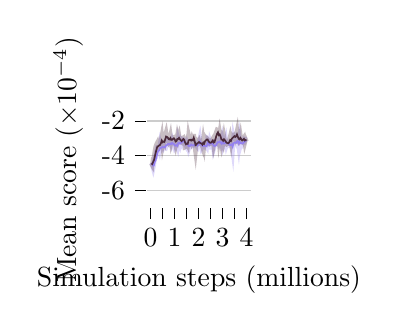
\begin{tikzpicture}

% \begin{axis}[
% axis background/.style={fill=white!82.7450980392157!black},
% axis line style={white},
% legend cell align={left},
% legend style={fill opacity=0.8, draw opacity=1, text opacity=1, at={(1,0.1)}, anchor=south east, draw=white!80!black},
% tick align=outside,
% tick pos=left,
% x grid style={white!69.0196078431373!black},
% xlabel={Timestep},
% xmajorgrids,
% xmin=-162030, xmax=4193970,
% xtick style={color=black},
% xtick={-500000,0,500000,1000000,1500000,2000000,2500000,3000000,3500000,4000000,4500000},
% xticklabels={-0.5M,0.0M,0.5M,1.0M,1.5M,2.0M,2.5M,3.0M,3.5M,4.0M,4.5M},
% y grid style={white!69.0196078431373!black},
% ylabel={Mean score},
% ymajorgrids,
% ymin=-10500, ymax=-1500,
% ytick style={color=black}
% ]
\definecolor{color0}{rgb}{0.83921568627451,0.152941176470588,0.156862745098039}
\definecolor{color1}{rgb}{0.12156862745098,0.966666666666667,0.205882352941177}
\definecolor{color2}{rgb}{0.580392156862745,0.503921568627451,0.941176470588235}
\definecolor{color3}{rgb}{0.290196078431372,0.166666666666667,0.23078431372549}

\begin{axis}[
    width=\figurewidth,
    height=\figureheight,
    axis background/.style={fill=white},
    axis line style={white},
    legend cell align={left},
    legend style={fill opacity=0.8, draw opacity=1, text opacity=1, at={(1,0.1)}, anchor=south east, draw=white!80!black},
    tick align=outside,
    tick pos=left,
    x grid style={white},
    xlabel={Simulation steps (millions)},
    xmajorgrids,
    xmin=-162030, 
    xmax=4193970,
    xtick style={color=black},
    xtick={-500000,0,500000,1000000,1500000,2000000,2500000,3000000,3500000,4000000,4500000},
    xticklabels={,0,,1,,2,,3,,4,},
    y grid style={white!80!black},
    ylabel={Mean score ($\times10^{-4}$)},
    ymajorgrids,
    ymin=-7000, 
    ymax=-1500,
    ytick={-10000,-8000,-6000,-4000,-2000},
    yticklabels={-10,-8,-6,-4,-2},
    ytick style={color=black},
    scaled y ticks = false,
    scaled x ticks = false
]
\addplot [ultra thick, color2, opacity=0.3, forget plot]
table {%
35970 -4429.5419921875
71970 -4551.52978515625
107970 -4734.90380859375
143970 -4494.49951171875
179970 -4107.19091796875
215970 -4093.01782226562
251970 -3709.23608398438
287970 -3528.4462890625
323970 -3535.58935546875
359970 -3693.3115234375
395970 -3350.1982421875
431970 -3584.38232421875
467970 -3450.05346679688
503970 -3458.7236328125
539970 -3565.31396484375
575970 -3464.95581054688
611970 -3507.54614257812
647970 -3254.36987304688
683970 -3384.14208984375
719970 -3247.28344726562
755970 -3332.84814453125
791970 -3369.81030273438
827970 -3238.7666015625
863970 -3371.3701171875
899970 -3177.56665039062
935970 -3386.20068359375
971970 -3342.9296875
1007970 -3545.79638671875
1043970 -3454.72021484375
1079970 -3357.62109375
1115970 -3501.25146484375
1151970 -3052.67749023438
1187970 -3231.93017578125
1223970 -3380.92163085938
1259970 -3161.50610351562
1295970 -3278.56396484375
1331970 -3056.56811523438
1367970 -3076.1875
1403970 -3289.32666015625
1439970 -3317.078125
1475970 -3425.78344726562
1511970 -3267.95849609375
1547970 -3424.02368164062
1583970 -3625.8828125
1619970 -3472.34521484375
1655970 -3365.06811523438
1691970 -3266.96533203125
1727970 -3462.2666015625
1763970 -3445.37670898438
1799970 -3402.03125
1835970 -3293.44458007812
1871970 -3331.9384765625
1907970 -3438.54223632812
1943970 -3505.03002929688
1979970 -3266.9130859375
2015970 -3228.69653320312
2051970 -2999.37084960938
2087970 -3369.078125
2123970 -3587.02734375
2159970 -3495.07543945312
2195970 -3487.0478515625
2231970 -3381.69995117188
2267970 -3472.57055664062
2303970 -3431.3564453125
2339970 -3512.87255859375
2375970 -2996.9560546875
2411970 -3030.24243164062
2447970 -3642.61108398438
2483970 -3177.76684570312
2519970 -3325.9375
2555970 -3312.09204101562
2591970 -3269.04711914062
2627970 -3640.0068359375
2663970 -3472.50073242188
2699970 -3387.80737304688
2735970 -3371.57177734375
2771970 -3121.4404296875
2807970 -3110.82397460938
2843970 -3258.05053710938
2879970 -3115.89428710938
2915970 -3297.0185546875
2951970 -3417.8271484375
2987970 -3103.56469726562
3023970 -3440.76342773438
3059970 -3287.1240234375
3095970 -3251.95751953125
3131970 -3046.8681640625
3167970 -3407.75756835938
3203970 -3264.89453125
3239970 -3365.00268554688
3275970 -3441.82446289062
3311970 -3445.9111328125
3347970 -3364.98657226562
3383970 -3302.4541015625
3419970 -3680.13500976562
3455970 -2981.98828125
3491970 -3221.5576171875
3527970 -3215.58422851562
3563970 -3300.01928710938
3599970 -3026
3635970 -3135.08642578125
3671970 -3499.23657226562
3707970 -3058.1630859375
3743970 -3428.19995117188
3779970 -3247.09204101562
3815970 -3355.41357421875
3851970 -3260.2490234375
3887970 -3109.14624023438
3923970 -3171.45825195312
3959970 -3052.91357421875
3995970 -3065.87841796875
};
\addplot [ultra thick, color3, opacity=0.3, forget plot]
table {%
35970 -4454.12744140625
71970 -4552.79541015625
107970 -4175.72802734375
143970 -4094.0693359375
179970 -3744.87451171875
215970 -3475.09448242188
251970 -3340.90454101562
287970 -3245.08325195312
323970 -3444.45678710938
359970 -3328.29272460938
395970 -3353.88159179688
431970 -3144.68115234375
467970 -2889.3056640625
503970 -3385.52709960938
539970 -3123.23461914062
575970 -3241.73803710938
611970 -2837.63427734375
647970 -2657.3154296875
683970 -2950.78295898438
719970 -3041.75659179688
755970 -3189.22509765625
791970 -3087.48022460938
827970 -2862.50634765625
863970 -3255.47290039062
899970 -3072.69604492188
935970 -2964.24389648438
971970 -2944.46630859375
1007970 -3154.13208007812
1043970 -3389.72924804688
1079970 -3135.2978515625
1115970 -2839.30053710938
1151970 -3054.82592773438
1187970 -2869.51318359375
1223970 -3189.2978515625
1259970 -3203.33935546875
1295970 -3237.12060546875
1331970 -2992.6708984375
1367970 -2962.04028320312
1403970 -3147.1240234375
1439970 -3509.32250976562
1475970 -3483.2255859375
1511970 -3236.73486328125
1547970 -3361.97924804688
1583970 -2820.06518554688
1619970 -3046.64428710938
1655970 -3067.38647460938
1691970 -3213.2392578125
1727970 -3019.90673828125
1763970 -3158.06396484375
1799970 -2754.1181640625
1835970 -3413.17309570312
1871970 -3774.57275390625
1907970 -3319.76293945312
1943970 -3172.6689453125
1979970 -3237.95263671875
2015970 -3144.68505859375
2051970 -3326.09130859375
2087970 -3338.06811523438
2123970 -3304.41088867188
2159970 -3475.90625
2195970 -3086.99169921875
2231970 -3402.77001953125
2267970 -2955.87573242188
2303970 -3041.96704101562
2339970 -3001.40454101562
2375970 -3051.30419921875
2411970 -3308.43115234375
2447970 -3338.5966796875
2483970 -3314.86669921875
2519970 -3237.99682617188
2555970 -3109.3232421875
2591970 -3028.25537109375
2627970 -3423.5654296875
2663970 -3191.24047851562
2699970 -2791.64990234375
2735970 -2648.15112304688
2771970 -2507.94287109375
2807970 -2530.1787109375
2843970 -3068.9990234375
2879970 -2722.36743164062
2915970 -3053.35815429688
2951970 -3357.57299804688
2987970 -3077.8798828125
3023970 -3254.20727539062
3059970 -2918.3251953125
3095970 -3203.41235351562
3131970 -3312.66284179688
3167970 -3348.8037109375
3203970 -3320.71557617188
3239970 -3307.99536132812
3275970 -3133.0029296875
3311970 -2925.47900390625
3347970 -3226.84741210938
3383970 -2832.9482421875
3419970 -2896.45092773438
3455970 -2850.9208984375
3491970 -2804.07397460938
3527970 -2997.25756835938
3563970 -2839.42602539062
3599970 -2603.27954101562
3635970 -3131.9873046875
3671970 -3207.39038085938
3707970 -3111.89477539062
3743970 -2852.54052734375
3779970 -3184.22436523438
3815970 -3215.82299804688
3851970 -3028.18310546875
3887970 -2956.10791015625
3923970 -3266.41918945312
3959970 -3062.765625
3995970 -3181.55102539062
};
\addplot [semithick, color2]
table {%
35970 -4429.5419921875
71970 -4478.337109375
107970 -4580.9637890625
143970 -4546.378078125
179970 -4370.7032140625
215970 -4259.62905734375
251970 -4039.471868
287970 -3835.061636425
323970 -3715.2727240425
359970 -3706.4882438005
395970 -3563.9722431553
431970 -3572.13627558068
467970 -3523.30315206716
503970 -3497.47134436529
539970 -3524.60839255668
575970 -3500.74735975276
611970 -3503.4668728829
647970 -3403.82807294849
683970 -3395.9536797066
719970 -3336.48558673021
755970 -3335.03060985062
791970 -3348.94248700412
827970 -3304.87213282748
863970 -3331.47132657149
899970 -3269.90945609914
935970 -3316.42594709698
971970 -3327.02744325819
1007970 -3414.53502064241
1043970 -3430.60909832295
1079970 -3401.41389649377
1115970 -3441.34892383376
1151970 -3285.88035039401
1187970 -3264.3002805489
1223970 -3310.94882067309
1259970 -3251.17173381011
1295970 -3262.12862622356
1331970 -3179.90442182789
1367970 -3138.41765309673
1403970 -3198.78125592054
1439970 -3246.10000355232
1475970 -3317.97338103764
1511970 -3297.96742706009
1547970 -3348.3899288923
1583970 -3459.38708233538
1619970 -3464.57033533873
1655970 -3424.76944729699
1691970 -3361.64780119069
1727970 -3401.89532133942
1763970 -3419.2878763974
1799970 -3412.38522583844
1835970 -3364.80896753431
1871970 -3351.66077114559
1907970 -3386.4133572186
1943970 -3433.86002604991
1979970 -3367.08125000495
2015970 -3311.72736328422
2051970 -3186.78475781428
2087970 -3259.70210468857
2123970 -3390.63220031314
2159970 -3432.40949596913
2195970 -3454.26483820648
2231970 -3425.23888339264
2267970 -3444.17155269183
2303970 -3439.0455097401
2339970 -3468.57632928156
2375970 -3279.92821944394
2411970 -3180.05390432261
2447970 -3365.07677618732
2483970 -3290.15280399364
2519970 -3304.46668239618
2555970 -3307.51682584396
2591970 -3292.12894316263
2627970 -3431.28010027258
2663970 -3447.7683531323
2699970 -3423.78396109813
2735970 -3402.89908759638
2771970 -3290.31562443283
2807970 -3218.51896450345
2843970 -3234.33159354582
2879970 -3186.95667097124
2915970 -3230.98142445774
2951970 -3305.71971404965
2987970 -3224.85770733604
3023970 -3311.21999549537
3059970 -3301.58160667222
3095970 -3281.73197181583
3131970 -3187.7864487145
3167970 -3275.77489657245
3203970 -3271.42275044347
3239970 -3308.85472448483
3275970 -3362.04261984715
3311970 -3395.59002503329
3347970 -3383.34864392622
3383970 -3350.99082698073
3419970 -3482.64850009469
3455970 -3282.38441255681
3491970 -3258.05369440909
3527970 -3241.0659080517
3563970 -3264.64725967477
3599970 -3169.18835580486
3635970 -3155.54758379542
3671970 -3293.0231791835
3707970 -3199.0791418851
3743970 -3290.72746559981
3779970 -3273.27329576614
3815970 -3306.12940714718
3851970 -3287.77725366331
3887970 -3216.32484829174
3923970 -3198.37820975629
3959970 -3140.19235554127
3995970 -3110.46678051226
};
% \addlegendentry{Training}
\addplot [semithick, color3]
table {%
35970 -4454.12744140625
71970 -4493.59462890625
107970 -4366.44798828125
143970 -4257.49652734375
179970 -4052.44772109375
215970 -3821.506425625
251970 -3629.26567178125
287970 -3475.59270385
323970 -3463.13833715375
359970 -3409.200092136
395970 -3387.07269200035
431970 -3290.11607613771
467970 -3129.79191130763
503970 -3232.08598662833
539970 -3188.54543963325
575970 -3209.8224786237
611970 -3060.94719811172
647970 -2899.49449074203
683970 -2920.00987803897
719970 -2968.70856354213
755970 -3056.91517718778
791970 -3069.14119615642
827970 -2986.48725675635
863970 -3094.08151421006
899970 -3085.52732649479
935970 -3037.01395449062
971970 -2999.99489613187
1007970 -3061.64976971037
1043970 -3192.88156104497
1079970 -3169.84807725198
1115970 -3037.62906119494
1151970 -3044.50780781071
1187970 -2974.50995812393
1223970 -3060.42511549936
1259970 -3117.59081148711
1295970 -3165.40272907977
1331970 -3096.30999682286
1367970 -3042.60211137497
1403970 -3084.41087619998
1439970 -3254.37552962624
1475970 -3345.91555215074
1511970 -3302.24327660295
1547970 -3326.13766518052
1583970 -3123.70867332706
1619970 -3092.88291883999
1655970 -3082.68434114774
1691970 -3134.90630781365
1727970 -3088.90648000069
1763970 -3116.56947393791
1799970 -2971.58894998775
1835970 -3148.2226082739
1871970 -3398.76266652684
1907970 -3367.16277569735
1943970 -3289.36524354341
1979970 -3268.80020081355
2015970 -3219.15414392563
2051970 -3261.92900979288
2087970 -3292.38465196948
2123970 -3297.19514665044
2159970 -3368.67958799026
2195970 -3256.00443248166
2231970 -3314.71066730149
2267970 -3171.17669334965
2303970 -3119.49283241604
2339970 -3072.25751585587
2375970 -3063.87618920102
2411970 -3161.69817445811
2447970 -3232.45757654987
2483970 -3265.42122561742
2519970 -3254.4514658392
2555970 -3196.40017637852
2591970 -3129.14225426461
2627970 -3246.91152443377
2663970 -3224.64310606651
2699970 -3051.44582457741
2735970 -2890.12794396519
2771970 -2737.25391481662
2807970 -2654.42383326497
2843970 -2820.25390933398
2879970 -2781.09931825664
2915970 -2890.00285267273
2951970 -3077.03091082239
2987970 -3077.37049961843
3023970 -3148.10520992731
3059970 -3056.19320408139
3095970 -3115.08086385508
3131970 -3194.1136550318
3167970 -3255.98967739408
3203970 -3281.8800369052
3239970 -3292.32616667437
3275970 -3228.59687187962
3311970 -3107.34972469027
3347970 -3155.14879965791
3383970 -3026.26857666975
3419970 -2974.3415170956
3455970 -2924.97326963236
3491970 -2876.61355162317
3527970 -2924.87115831765
3563970 -2890.69310514684
3599970 -2775.72767949435
3635970 -2918.23152957161
3671970 -3033.89507008672
3707970 -3065.09495220828
3743970 -2980.07318226247
3779970 -3061.73365545123
3815970 -3123.36939248949
3851970 -3085.29487768119
3887970 -3033.62009067122
3923970 -3126.73973018398
3959970 -3101.15008811039
3995970 -3133.31046302248
};
% \addlegendentry{Evaluation}
\end{axis}

\end{tikzpicture}
}
        \caption{OV5}
        \label{fig:OV5}
    \end{subfigure}
    \begin{subfigure}[t]{0.24\textwidth}
        \centering
        \setlength{\figureheight}{0.8\textwidth}
        \setlength{\figurewidth}{\textwidth}
        \footnotesize{% This file was created by tikzplotlib v0.9.1.
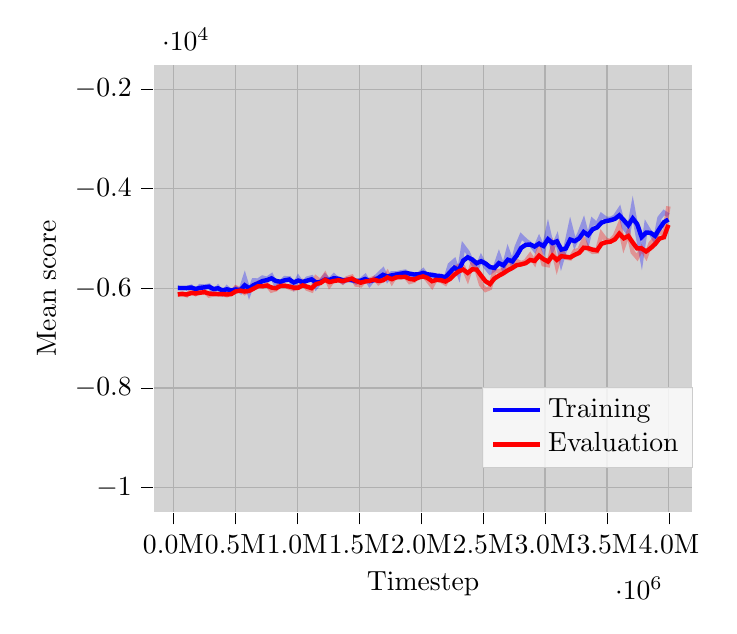
\begin{tikzpicture}

\begin{axis}[
axis background/.style={fill=white!82.7450980392157!black},
axis line style={white},
legend cell align={left},
legend style={fill opacity=0.8, draw opacity=1, text opacity=1, at={(1,0.1)}, anchor=south east, draw=white!80!black},
tick align=outside,
tick pos=left,
x grid style={white!69.0196078431373!black},
xlabel={Timestep},
xmajorgrids,
xmin=-162030, xmax=4193970,
xtick style={color=black},
xtick={-500000,0,500000,1000000,1500000,2000000,2500000,3000000,3500000,4000000,4500000},
xticklabels={-0.5M,0.0M,0.5M,1.0M,1.5M,2.0M,2.5M,3.0M,3.5M,4.0M,4.5M},
y grid style={white!69.0196078431373!black},
ylabel={Mean score},
ymajorgrids,
ymin=-10500, ymax=-1500,
ytick style={color=black}
]
\addplot [ultra thick, blue, opacity=0.3, forget plot]
table {%
35970 -5991.865234375
71970 -5995.392578125
107970 -5994.5078125
143970 -5968.001953125
179970 -6054.9091796875
215970 -5956.39892578125
251970 -5963.923828125
287970 -5947.140625
323970 -6082.361328125
359970 -5978.65625
395970 -6102.05615234375
431970 -5988.3447265625
467970 -6071.6943359375
503970 -5994.8759765625
539970 -6060.4775390625
575970 -5789.15478515625
611970 -6088.0283203125
647970 -5839.47900390625
683970 -5843.189453125
719970 -5784.57470703125
755970 -5808.11376953125
791970 -5745.9208984375
827970 -5930.4912109375
863970 -5888.90380859375
899970 -5795.484375
935970 -5799.177734375
971970 -5968.841796875
1007970 -5788.14990234375
1043970 -5914.52001953125
1079970 -5804.470703125
1115970 -5780.025390625
1151970 -5973.74462890625
1187970 -5861.03369140625
1223970 -5750.888671875
1259970 -5837.6611328125
1295970 -5745.1171875
1331970 -5826.12060546875
1367970 -5874.7607421875
1403970 -5825.64013671875
1439970 -5837.52880859375
1475970 -5880.662109375
1511970 -5838.14306640625
1547970 -5760.20166015625
1583970 -5915.4013671875
1619970 -5806.59521484375
1655970 -5720.8291015625
1691970 -5635.32470703125
1727970 -5819.2001953125
1763970 -5699.23388671875
1799970 -5700.35400390625
1835970 -5679.63330078125
1871970 -5664.23486328125
1907970 -5729.40869140625
1943970 -5746.25439453125
1979970 -5716.4521484375
2015970 -5643.72314453125
2051970 -5763.41064453125
2087970 -5742.28759765625
2123970 -5772.994140625
2159970 -5763.18017578125
2195970 -5816.79638671875
2231970 -5526.5966796875
2267970 -5447.875
2303970 -5705.82177734375
2339970 -5157.884765625
2375970 -5275.78466796875
2411970 -5483.91357421875
2447970 -5610.357421875
2483970 -5393.8857421875
2519970 -5570.75537109375
2555970 -5680.13134765625
2591970 -5615.0234375
2627970 -5349.271484375
2663970 -5602.5908203125
2699970 -5258.439453125
2735970 -5505.55517578125
2771970 -5167.10986328125
2807970 -4952.591796875
2843970 -5039.97412109375
2879970 -5106.4111328125
2915970 -5220.41845703125
2951970 -5016.10205078125
2987970 -5220.7734375
3023970 -4810.22412109375
3059970 -5208.31298828125
3095970 -5002.830078125
3131970 -5467.69384765625
3167970 -5167.68310546875
3203970 -4752.2578125
3239970 -5098.873046875
3275970 -4911.802734375
3311970 -4679.2919921875
3347970 -5023.9775390625
3383970 -4642.3720703125
3419970 -4720.43603515625
3455970 -4534.828125
3491970 -4602.5068359375
3527970 -4608.0146484375
3563970 -4562.2919921875
3599970 -4427.525390625
3635970 -4777.19775390625
3671970 -4888.47119140625
3707970 -4389.5224609375
3743970 -4881.2685546875
3779970 -5364.025390625
3815970 -4743.2373046875
3851970 -4891.81396484375
3887970 -5039.6806640625
3923970 -4587.27587890625
3959970 -4475.78271484375
3995970 -4533.9228515625
};
\addplot [ultra thick, red, opacity=0.3, forget plot]
table {%
35970 -6121.56689453125
71970 -6102.22998046875
107970 -6137.7744140625
143970 -6049.67626953125
179970 -6115.029296875
215970 -6065.6630859375
251970 -6060.7080078125
287970 -6143.87353515625
323970 -6120.75
359970 -6120.515625
395970 -6113.7080078125
431970 -6137.92626953125
467970 -6101.32470703125
503970 -5980.59912109375
539970 -6020.443359375
575970 -6092.412109375
611970 -6029.9326171875
647970 -5936.904296875
683970 -5888.04052734375
719970 -5956.9873046875
755970 -5920.41552734375
791970 -6045.07275390625
827970 -6019.1484375
863970 -5887.03125
899970 -5942.529296875
935970 -5984.8359375
971970 -6016.8515625
1007970 -5989.03173828125
1043970 -5872.3505859375
1079970 -6006.66162109375
1115970 -6040.12451171875
1151970 -5789.99560546875
1187970 -5859.76220703125
1223970 -5733.34814453125
1259970 -5939.3955078125
1295970 -5821.9091796875
1331970 -5813.47314453125
1367970 -5881.11279296875
1403970 -5793.63037109375
1439970 -5765.4033203125
1475970 -5924.5595703125
1511970 -5937.5048828125
1547970 -5826.75146484375
1583970 -5827.20068359375
1619970 -5792.138671875
1655970 -5889.9228515625
1691970 -5819.37158203125
1727970 -5694.2939453125
1763970 -5868.1142578125
1799970 -5722.982421875
1835970 -5768.822265625
1871970 -5760.35693359375
1907970 -5871.7197265625
1943970 -5845.35205078125
1979970 -5720.12158203125
2015970 -5728.03662109375
2051970 -5836.20068359375
2087970 -5952.826171875
2123970 -5792.63623046875
2159970 -5845.802734375
2195970 -5901.36767578125
2231970 -5739.4560546875
2267970 -5597.93310546875
2303970 -5555.03955078125
2339970 -5570.6552734375
2375970 -5791.90087890625
2411970 -5513.7666015625
2447970 -5624.73583984375
2483970 -5925.7490234375
2519970 -6030.849609375
2555970 -5993.95947265625
2591970 -5638.0859375
2627970 -5660.37548828125
2663970 -5624.60205078125
2699970 -5549.5439453125
2735970 -5519.04736328125
2771970 -5450.10009765625
2807970 -5496.5146484375
2843970 -5456.8154296875
2879970 -5336.18115234375
2915970 -5476.46533203125
2951970 -5190.06884765625
2987970 -5516.7607421875
3023970 -5534.873046875
3059970 -5169.10498046875
3095970 -5552.916015625
3131970 -5244.68798828125
3167970 -5383.35107421875
3203970 -5396.90576171875
3239970 -5252.11474609375
3275970 -5228.42919921875
3311970 -5029.4365234375
3347970 -5204.73486328125
3383970 -5267.66455078125
3419970 -5259.8134765625
3455970 -4910.21630859375
3491970 -5028.59912109375
3527970 -5045.40869140625
3563970 -4947.04833984375
3599970 -4729.0771484375
3635970 -5135.41650390625
3671970 -4881.318359375
3707970 -5274.505859375
3743970 -5378.11865234375
3779970 -5198.7021484375
3815970 -5349.9384765625
3851970 -5097.6455078125
3887970 -4987.97412109375
3923970 -4835.74365234375
3959970 -4929.84228515625
3995970 -4354.03076171875
};
\addplot [ultra thick, blue]
table {%
35970 -5991.865234375
71970 -5993.276171875
107970 -5993.768828125
143970 -5983.462078125
179970 -6012.04091875
215970 -5989.7841215625
251970 -5979.4400041875
287970 -5966.5202525125
323970 -6012.8566827575
359970 -5999.1765096545
395970 -6040.3283667302
431970 -6019.53491066312
467970 -6040.39868077287
503970 -6022.18959908872
539970 -6037.50477507823
575970 -5938.16477910944
611970 -5998.11019559066
647970 -5934.6577189169
683970 -5898.07041260014
719970 -5852.67213037258
755970 -5834.84878603605
791970 -5799.27763099663
827970 -5851.76306297298
863970 -5866.61936122129
899970 -5838.16536673277
935970 -5822.57031378966
971970 -5881.0789070238
1007970 -5843.90730515178
1043970 -5872.15239090357
1079970 -5845.07971579214
1115970 -5819.05798572528
1151970 -5880.93264299767
1187970 -5872.9730623611
1223970 -5824.13930616666
1259970 -5829.548036825
1295970 -5795.775697095
1331970 -5807.9136604445
1367970 -5834.6524931417
1403970 -5831.04755057252
1439970 -5833.64005378101
1475970 -5852.44887601861
1511970 -5846.72655217366
1547970 -5812.1165953667
1583970 -5853.43050409502
1619970 -5834.69638839451
1655970 -5789.14947366171
1691970 -5727.61956700952
1727970 -5764.25181833071
1763970 -5738.24464568593
1799970 -5723.08838897406
1835970 -5705.70635369693
1871970 -5689.11775753066
1907970 -5705.2341310809
1943970 -5721.64223646104
1979970 -5719.56620125162
2015970 -5689.22897856347
2051970 -5718.90164495059
2087970 -5728.25602603285
2123970 -5746.15127186971
2159970 -5752.96283343433
2195970 -5778.4962547481
2231970 -5677.73642472386
2267970 -5585.79185483431
2303970 -5633.80382383809
2339970 -5443.43620055285
2375970 -5376.37558751921
2411970 -5419.39078219903
2447970 -5495.77743806942
2483970 -5455.02075971665
2519970 -5501.31460426749
2555970 -5572.84130162299
2591970 -5589.7141559738
2627970 -5493.53708733428
2663970 -5537.15858052557
2699970 -5425.67092956534
2735970 -5457.6246280517
2771970 -5341.41872214352
2807970 -5185.88795203611
2843970 -5127.52241965917
2879970 -5119.0779049205
2915970 -5159.6141257648
2951970 -5102.20929577138
2987970 -5149.63495246283
3023970 -5013.8706199152
3059970 -5091.64756726162
3095970 -5056.12057160697
3131970 -5220.74988202668
3167970 -5199.52317140351
3203970 -5020.61702784211
3239970 -5051.91943545526
3275970 -4995.87275502316
3311970 -4869.24044988889
3347970 -4931.13528555834
3383970 -4815.62999946
3419970 -4777.5524137385
3455970 -4680.4626982431
3491970 -4649.28035332086
3527970 -4632.77407136752
3563970 -4604.58123969551
3599970 -4533.75890006731
3635970 -4631.13444160288
3671970 -4734.06914152423
3707970 -4596.25046928954
3743970 -4710.25770344872
3779970 -4971.76477831923
3815970 -4880.35378886654
3851970 -4884.93785925742
3887970 -4946.83498117946
3923970 -4803.01134027017
3959970 -4672.1198900996
3995970 -4616.84107468476
};
\addlegendentry{Training}
\addplot [ultra thick, red]
table {%
35970 -6121.56689453125
71970 -6113.83212890625
107970 -6123.40904296875
143970 -6093.91593359375
179970 -6102.36127890625
215970 -6087.68200171875
251970 -6076.89240415625
287970 -6103.68485655625
323970 -6110.51091393375
359970 -6114.51279836025
395970 -6114.19088214115
431970 -6123.68503709719
467970 -6114.74090507081
503970 -6061.08419147999
539970 -6044.82785863799
575970 -6063.8615589328
611970 -6050.28998223468
647970 -6004.93570809081
683970 -5958.17763579198
719970 -5957.70150335019
755970 -5942.78711294761
791970 -5983.70136933107
827970 -5997.88019659864
863970 -5953.54061795918
899970 -5949.13608952551
935970 -5963.41602871531
971970 -5984.79024222918
1007970 -5986.48684065001
1043970 -5940.83233876501
1079970 -5967.1640516965
1115970 -5996.3482357054
1151970 -5913.80718361074
1187970 -5892.18919297894
1223970 -5828.65277359987
1259970 -5872.94986728492
1295970 -5852.53359224595
1331970 -5836.90941316007
1367970 -5854.59076508354
1403970 -5830.20660748763
1439970 -5804.28529261758
1475970 -5852.39500369554
1511970 -5886.43895534233
1547970 -5862.5639591429
1583970 -5848.41864892324
1619970 -5825.90665810394
1655970 -5851.51313548736
1691970 -5838.65651410492
1727970 -5780.91148658795
1763970 -5815.79259507777
1799970 -5778.66852579666
1835970 -5774.730021728
1871970 -5768.9807864743
1907970 -5810.07636250958
1943970 -5824.18663781825
1979970 -5782.56061550345
2015970 -5760.75101773957
2051970 -5790.93088408124
2087970 -5855.68899919874
2123970 -5830.46789170675
2159970 -5836.60182877405
2195970 -5862.50816757693
2231970 -5813.28732242116
2267970 -5727.14563564019
2303970 -5658.30320169662
2339970 -5623.24403039297
2375970 -5690.70676979828
2411970 -5619.93070250397
2447970 -5621.85275743988
2483970 -5743.41126383893
2519970 -5858.38660205336
2555970 -5912.61575029451
2591970 -5802.80382517671
2627970 -5745.83249041852
2663970 -5697.34031456361
2699970 -5638.22176686317
2735970 -5590.5520054304
2771970 -5534.37124232074
2807970 -5519.22860476744
2843970 -5494.26333473547
2879970 -5431.03046177878
2915970 -5449.20440987977
2951970 -5345.55018499036
2987970 -5414.03440786922
3023970 -5462.36986347153
3059970 -5345.06391027042
3095970 -5428.20475241225
3131970 -5354.79804675985
3167970 -5366.21925774341
3203970 -5378.49385933355
3239970 -5327.94221403763
3275970 -5288.13700811008
3311970 -5184.65681424105
3347970 -5192.68803385713
3383970 -5222.67864062678
3419970 -5237.53257500107
3455970 -5106.60606843814
3491970 -5075.40328950038
3527970 -5063.40545026273
3563970 -5016.86260609514
3599970 -4901.74842303208
3635970 -4995.21565538175
3671970 -4949.65673697905
3707970 -5079.59638593743
3743970 -5199.00529249996
3779970 -5198.88403487497
3815970 -5259.30581154998
3851970 -5194.64169005499
3887970 -5111.97466247049
3923970 -5001.4822584198
3959970 -4972.82626911438
3995970 -4725.30806615613
};
\addlegendentry{Evaluation}
\end{axis}

\end{tikzpicture}
}
        \caption{OV15}
        \label{fig:OV15}
    \end{subfigure}
    \begin{subfigure}[t]{0.24\textwidth}
        \centering
        \setlength{\figureheight}{0.8\textwidth}
        \setlength{\figurewidth}{\textwidth}
        \footnotesize{% This file was created by tikzplotlib v0.9.1.
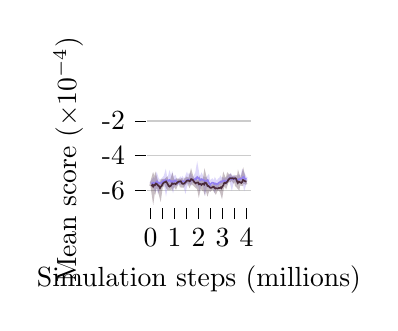
\begin{tikzpicture}

% \begin{axis}[
% axis background/.style={fill=white!82.7450980392157!black},
% axis line style={white},
% legend cell align={left},
% legend style={fill opacity=0.8, draw opacity=1, text opacity=1, at={(1,0.1)}, anchor=south east, draw=white!80!black},
% tick align=outside,
% tick pos=left,
% x grid style={white!69.0196078431373!black},
% xlabel={Simulation steps},
% xmajorgrids,
% xmin=-162030, xmax=4193970,
% xtick style={color=black},
% xtick={-500000,0,500000,1000000,1500000,2000000,2500000,3000000,3500000,4000000,4500000},
% xticklabels={-0.5M,0.0M,0.5M,1.0M,1.5M,2.0M,2.5M,3.0M,3.5M,4.0M,4.5M},
% y grid style={white!69.0196078431373!black},
% ylabel={Mean score},
% ymajorgrids,
% ymin=-7000, ymax=-1500,
% ytick style={color=black}
% ]
\definecolor{color0}{rgb}{0.83921568627451,0.152941176470588,0.156862745098039}
\definecolor{color1}{rgb}{0.12156862745098,0.966666666666667,0.205882352941177}
\definecolor{color2}{rgb}{0.580392156862745,0.503921568627451,0.941176470588235}
\definecolor{color3}{rgb}{0.290196078431372,0.166666666666667,0.23078431372549}

\begin{axis}[
    width=\figurewidth,
    height=\figureheight,
    axis background/.style={fill=white},
    axis line style={white},
    legend cell align={left},
    legend style={fill opacity=0.8, draw opacity=1, text opacity=1, at={(1,0.1)}, anchor=south east, draw=white!80!black},
    tick align=outside,
    tick pos=left,
    x grid style={white},
    xlabel={Simulation steps (millions)},
    xmajorgrids,
    xmin=-162030, 
    xmax=4193970,
    xtick style={color=black},
    xtick={-500000,0,500000,1000000,1500000,2000000,2500000,3000000,3500000,4000000,4500000},
    xticklabels={,0,,1,,2,,3,,4,},
    y grid style={white!80!black},
    ylabel={Mean score ($\times10^{-4}$)},
    ymajorgrids,
    ymin=-7000, 
    ymax=-1500,
    ytick={-10000,-8000,-6000,-4000,-2000},
    yticklabels={-10,-8,-6,-4,-2},
    ytick style={color=black},
    scaled y ticks = false,
    scaled x ticks = false
]
\addplot [ultra thick, color2, opacity=0.3, forget plot]
table {%
35970 -5645.6240234375
71970 -5559.96533203125
107970 -5497.29833984375
143970 -5615.23486328125
179970 -5728.1328125
215970 -5509.2109375
251970 -5359.28759765625
287970 -5525.283203125
323970 -5739.66064453125
359970 -5562.20361328125
395970 -5630.9501953125
431970 -5607.13232421875
467970 -5474.21142578125
503970 -5442.60986328125
539970 -5386.1552734375
575970 -5506.22998046875
611970 -5335.59033203125
647970 -5633.28076171875
683970 -5356.49560546875
719970 -5395.96240234375
755970 -5526.060546875
791970 -5339.80615234375
827970 -5534.31884765625
863970 -5616.02392578125
899970 -5424.69873046875
935970 -5630.638671875
971970 -5416.3623046875
1007970 -5354.1953125
1043970 -5473.912109375
1079970 -5616.48681640625
1115970 -5600.287109375
1151970 -5588.9541015625
1187970 -5499.33447265625
1223970 -5440.30908203125
1259970 -5547.2666015625
1295970 -5515.75244140625
1331970 -5429.12646484375
1367970 -5511.97021484375
1403970 -5502.6259765625
1439970 -5677.0048828125
1475970 -5420.2490234375
1511970 -5294.2294921875
1547970 -5436.5947265625
1583970 -5336.341796875
1619970 -5504.529296875
1655970 -5533.61279296875
1691970 -5301.9248046875
1727970 -5382.5625
1763970 -5403.2978515625
1799970 -5440.07177734375
1835970 -5345.14404296875
1871970 -5244.96337890625
1907970 -5383.5634765625
1943970 -5086.2490234375
1979970 -5371.70068359375
2015970 -5336.89794921875
2051970 -5569.34912109375
2087970 -5405.87841796875
2123970 -5292.8076171875
2159970 -5415.93115234375
2195970 -5466.677734375
2231970 -5437.17529296875
2267970 -5674.79248046875
2303970 -5407.140625
2339970 -5433.3369140625
2375970 -5368.0283203125
2411970 -5709.28173828125
2447970 -5757.37451171875
2483970 -5783.310546875
2519970 -5535.3740234375
2555970 -5497.11865234375
2591970 -5572.72998046875
2627970 -5596.14990234375
2663970 -5741.4267578125
2699970 -5569.806640625
2735970 -5663.248046875
2771970 -5729.1005859375
2807970 -5561.9609375
2843970 -5493.01904296875
2879970 -5534.33935546875
2915970 -5430.54736328125
2951970 -5525.5859375
2987970 -5495.46923828125
3023970 -5399.0537109375
3059970 -5404.29345703125
3095970 -5527.62548828125
3131970 -5543.587890625
3167970 -5402.84912109375
3203970 -5400.5234375
3239970 -5338.74853515625
3275970 -5243.27197265625
3311970 -5202.1474609375
3347970 -5294.470703125
3383970 -5502.22705078125
3419970 -5296.13330078125
3455970 -5273.345703125
3491970 -5359.8681640625
3527970 -5389.71435546875
3563970 -5398.82958984375
3599970 -5452.193359375
3635970 -5358.61767578125
3671970 -5407.39892578125
3707970 -5280.9189453125
3743970 -5325.734375
3779970 -5333.197265625
3815970 -5335.4765625
3851970 -5123.26806640625
3887970 -5217.54052734375
3923970 -5512.7236328125
3959970 -5349.4755859375
3995970 -5383.837890625
};
\addplot [ultra thick, color3, opacity=0.3, forget plot]
table {%
35970 -5775.3779296875
71970 -5595.23095703125
107970 -5939.06689453125
143970 -5565.06982421875
179970 -5733.13134765625
215970 -5473.57275390625
251970 -5648.6337890625
287970 -5787.56103515625
323970 -5824.3935546875
359970 -5835.64892578125
395970 -6030.17041015625
431970 -5669.65771484375
467970 -5682.537109375
503970 -5490.87841796875
539970 -5476.52294921875
575970 -5493.61376953125
611970 -5504.10693359375
647970 -5454.50048828125
683970 -5692.470703125
719970 -5806.52978515625
755970 -5871.6904296875
791970 -5866.70458984375
827970 -5732.3828125
863970 -5615.36962890625
899970 -5460.8994140625
935970 -5686.92724609375
971970 -5602.544921875
1007970 -5612.869140625
1043970 -5696.21044921875
1079970 -5571.70849609375
1115970 -5461.3408203125
1151970 -5472.00341796875
1187970 -5465.966796875
1223970 -5491.18603515625
1259970 -5473.013671875
1295970 -5720.83935546875
1331970 -5725.95947265625
1367970 -5627.0009765625
1403970 -5596.61083984375
1439970 -5500.408203125
1475970 -5423.0458984375
1511970 -5376.88232421875
1547970 -5408.9296875
1583970 -5444.81005859375
1619970 -5555.91162109375
1655970 -5420.04931640625
1691970 -5222.1953125
1727970 -5397.40673828125
1763970 -5469.28955078125
1799970 -5606.32958984375
1835970 -5641.70458984375
1871970 -5689.4072265625
1907970 -5509.328125
1943970 -5562.4208984375
1979970 -5548.9921875
2015970 -5810.85693359375
2051970 -5586.1923828125
2087970 -5703.275390625
2123970 -5769.95556640625
2159970 -5553.7568359375
2195970 -5586.85693359375
2231970 -5750.8681640625
2267970 -5404.7373046875
2303970 -5612.125
2339970 -5740.748046875
2375970 -5922.64794921875
2411970 -5758.87158203125
2447970 -5886.91943359375
2483970 -5929.54150390625
2519970 -5883.97412109375
2555970 -5815.8857421875
2591970 -5789.212890625
2627970 -5782.80224609375
2663970 -5921.0146484375
2699970 -5996.71728515625
2735970 -5868.00244140625
2771970 -5926.8291015625
2807970 -5894.50634765625
2843970 -5834.24658203125
2879970 -5893.39404296875
2915970 -5785.0478515625
2951970 -5956.43603515625
2987970 -5643.7646484375
3023970 -5665.29833984375
3059970 -5396.99365234375
3095970 -5526.79638671875
3131970 -5625.67138671875
3167970 -5473.380859375
3203970 -5450.7001953125
3239970 -5232.22705078125
3275970 -5289.8662109375
3311970 -5247.8486328125
3347970 -5342.95263671875
3383970 -5297.70458984375
3419970 -5305.83349609375
3455970 -5385.0986328125
3491970 -5301.62255859375
3527970 -5285.1083984375
3563970 -5410.05322265625
3599970 -5684.388671875
3635970 -5740.455078125
3671970 -5393.92333984375
3707970 -5560.09228515625
3743970 -5602.86865234375
3779970 -5615.1552734375
3815970 -5442.56201171875
3851970 -5245.53125
3887970 -5482.88134765625
3923970 -5516.01513671875
3959970 -5546.46435546875
3995970 -5525.37841796875
};
\addplot [semithick, color2]
table {%
35970 -5645.6240234375
71970 -5611.360546875
107970 -5565.7356640625
143970 -5585.53534375
179970 -5642.57433125
215970 -5589.22897375
251970 -5497.2524233125
287970 -5508.4647352375
323970 -5600.943098955
359970 -5585.4473046855
395970 -5603.6484609363
431970 -5605.04200624928
467970 -5552.70977406207
503970 -5508.66980974974
539970 -5459.66399522484
575970 -5478.29038932241
611970 -5421.21036640594
647970 -5506.03852453107
683970 -5446.22135690614
719970 -5426.11777508118
755970 -5466.09488379871
791970 -5415.57939121673
827970 -5463.07517379254
863970 -5524.25467458802
899970 -5484.43229694031
935970 -5542.91484691419
971970 -5492.29383002351
1007970 -5437.05442301411
1043970 -5451.79749755846
1079970 -5517.67322509758
1115970 -5550.71877880855
1151970 -5566.01290791013
1187970 -5539.34153380858
1223970 -5499.72855309765
1259970 -5518.74377248359
1295970 -5517.54724005265
1331970 -5482.17892996909
1367970 -5494.09544391896
1403970 -5497.50765697637
1439970 -5569.30654731082
1475970 -5509.68353776149
1511970 -5423.5019195319
1547970 -5428.73904234414
1583970 -5391.78014415648
1619970 -5436.87980524389
1655970 -5475.57300033383
1691970 -5406.1137220753
1727970 -5396.69323324518
1763970 -5399.33508057211
1799970 -5415.62975928077
1835970 -5387.43547275596
1871970 -5330.44663521607
1907970 -5351.69337175464
1943970 -5245.51563242779
1979970 -5295.98965289417
2015970 -5312.352971424
2051970 -5415.1514312919
2087970 -5411.44222596264
2123970 -5363.98838245258
2159970 -5384.76549040905
2195970 -5417.53038799543
2231970 -5425.38834998476
2267970 -5525.15000217835
2303970 -5477.94625130701
2339970 -5460.10251640921
2375970 -5423.27283797052
2411970 -5537.67639809481
2447970 -5625.55564354439
2483970 -5688.65760487663
2519970 -5627.34417230098
2555970 -5575.25396431809
2591970 -5574.24437077835
2627970 -5583.00658340451
2663970 -5646.37465316771
2699970 -5615.74744815062
2735970 -5634.74768764037
2771970 -5672.48884695922
2807970 -5628.27768317553
2843970 -5574.17422709282
2879970 -5558.24027844319
2915970 -5507.16311237842
2951970 -5514.53224242705
2987970 -5506.90704076873
3023970 -5463.76570883624
3059970 -5439.97680811424
3095970 -5475.03628018105
3131970 -5502.45692435863
3167970 -5462.61380305268
3203970 -5437.77765683161
3239970 -5398.16600816146
3275970 -5336.20839395938
3311970 -5282.58402075063
3347970 -5287.33869370038
3383970 -5373.29403653273
3419970 -5342.42974223214
3455970 -5314.79612658928
3491970 -5332.82494157857
3527970 -5355.58070713464
3563970 -5372.88026021828
3599970 -5404.60549988097
3635970 -5386.21037024108
3671970 -5394.68579245715
3707970 -5349.17905359929
3743970 -5339.80118215957
3779970 -5337.15961554574
3815970 -5336.48639432745
3851970 -5251.19906315897
3887970 -5237.73564883288
3923970 -5347.73084242473
3959970 -5348.42873982984
3995970 -5362.5924001479
};
%\addlegendentry{Training}
\addplot [semithick, color3]
table {%
35970 -5775.3779296875
71970 -5703.319140625
107970 -5797.6182421875
143970 -5704.598875
179970 -5716.0118640625
215970 -5619.03622
251970 -5630.875247625
287970 -5693.5495626375
323970 -5745.8871594575
359970 -5781.791865987
395970 -5881.1432836547
431970 -5796.54905613032
467970 -5750.94427742819
503970 -5646.91793364442
539970 -5578.75993987415
575970 -5544.70147173699
611970 -5528.46365647969
647970 -5498.87838920032
683970 -5576.31531477019
719970 -5668.40110292461
755970 -5749.71683362977
791970 -5796.51193611536
827970 -5770.86028666922
863970 -5708.66402356403
899970 -5609.55817976342
935970 -5640.50580629555
971970 -5625.32145252733
1007970 -5620.3405277664
1043970 -5650.68849634734
1079970 -5619.0964962459
1115970 -5555.99422587254
1151970 -5522.39790271103
1187970 -5499.82546037661
1223970 -5496.36969028847
1259970 -5487.02728292308
1295970 -5580.55211194135
1331970 -5638.71505622731
1367970 -5634.02942436139
1403970 -5619.06199055433
1439970 -5571.6004755826
1475970 -5512.17864472456
1511970 -5458.06011652224
1547970 -5438.40794491334
1583970 -5440.9687903855
1619970 -5486.9459226688
1655970 -5460.18728016378
1691970 -5364.99049309827
1727970 -5377.95699117146
1763970 -5414.49001501538
1799970 -5491.22584494673
1835970 -5551.41734290554
1871970 -5606.61329636832
1907970 -5567.69922782099
1943970 -5565.5878960676
1979970 -5558.94961264056
2015970 -5659.71254102183
2051970 -5630.3044777381
2087970 -5659.49284289286
2123970 -5703.67793229822
2159970 -5643.70949375393
2195970 -5620.96846968986
2231970 -5672.92834743891
2267970 -5565.65193033835
2303970 -5584.24115820301
2339970 -5646.84391367181
2375970 -5757.16552789058
2411970 -5757.84794954685
2447970 -5809.47654316561
2483970 -5857.50252746187
2519970 -5868.09116491462
2555970 -5847.20899582377
2591970 -5824.01055374426
2627970 -5807.52723068406
2663970 -5852.92219778543
2699970 -5910.44023273376
2735970 -5893.46511620276
2771970 -5906.81071034665
2807970 -5901.88896527049
2843970 -5874.8320119748
2879970 -5882.25682437238
2915970 -5843.37323524843
2951970 -5888.59835521156
2987970 -5790.66487250193
3023970 -5740.51825943866
3059970 -5603.1084166007
3095970 -5572.58360464792
3131970 -5593.81871747625
3167970 -5545.64357423575
3203970 -5507.66622266645
3239970 -5397.49055391237
3275970 -5354.44081672242
3311970 -5311.80394315845
3347970 -5324.26342058257
3383970 -5313.63988828704
3419970 -5310.51733140973
3455970 -5340.34985197084
3491970 -5324.85893462
3527970 -5308.958720147
3563970 -5349.3965211507
3599970 -5483.39338144042
3635970 -5586.21806011425
3671970 -5509.30017200605
3707970 -5529.61701726613
3743970 -5558.91767129718
3779970 -5581.41271215331
3815970 -5525.87243197948
3851970 -5413.73595918769
3887970 -5441.39411457511
3923970 -5471.24252343257
3959970 -5501.33125624704
3995970 -5510.95012093572
};
%\addlegendentry{Evaluation}
\end{axis}

\end{tikzpicture}
}
        \caption{OV25}
        \label{fig:OV25}
    \end{subfigure}
    \caption{Simulation results where we show the training in perturbance-free environment, and 12 cases where we analyze the effect of a modified environment (fixed and variable perturbances on both sensing and actuation) on 5, 15 and 25 agents. The total number of agents is 30 in all cases. The legend is common across all graphs and has been omitted in subfigures (b) through (m) to improve readability.}
    \label{fig:main_results}
\end{figure*}

\section{Experimentation and Results}
\label{sec:results}

In this section, we describe the training parameters utilized through our simulations, and the ways in which the environments have been modified to introduce disturbances in both sensors and actuators. We then present the results of multiple simulations where different numbers of agents have been trained in different environments but treated equally from the point of view of the collaborative learning process.

\subsection{Training Method}

The maximal number of steps in one episode is set to 1200, and the maximum number of steps for the whole training process is set to 4 million. If the gripper contacts the object or approaches it at a very small distance (0.008\,m), the episode will be terminated. The final score for this episode is thus calculated by summing all the rewards obtained in all the steps until termination.

The initial reward is set as -1000 for each step if the distance is larger than 1\,m. However, if the distance between the finger on the gripper and the object is smaller than 1\,m, the reward is computed as $reward_{raw} = -10\cdot distance$. Moreover, we also add the cost of each step, in order to encourage the gripper to approach the target as soon as possible. The cost of each step is set as 1. Therefore, the final reward for this step is hence: $ reward_{final} = -10\cdot distance - 1$, where the distance is given in meters. If the gripper finally contacts its target or approach it in a threshold, we give it a significantly larger reward (1000) to help the model learn faster and clearly.

In total, in our simulations, we utilize 30 agents parallelized on the GPU processes to produce experience data based on a vectorized environment. Therefore, these agents can represent a multi-robot system learning a collaborative RL task. We give different settings on individual environments to manually simulate the possible perturbations that robots find in real-world scenarios. 


\subsection{Calibration and Accuracy Noises}

To emulate the practical noises and errors that robots could encounter when training an RL algorithm, we consider the following four types of perturbations, for each of which we generate a different environment to expose a variable number of robots to: fixed input errors on all the nine elements by $0.005\,m$, uniformly distributed sensing errors in the interval $[0.005\,m, 0.01\,m]$, fixed output errors modifying the gripper actuators by an offset of $0.005\,m$ on the $x$ axis, and uniformly distributed output errors in the interval $[0.005\,m, 0.01\,m]$. It should be noted that the uniform distributed errors on input and output could be different in each step, which can be regarded as inaccurate sensing errors, or reduced repeatability in the actuation of real robots.

Moreover, in order to further analyze how more extreme cases affect the collaborative learning process, we also consider fixed disturbances on larger magnitude (0.015\,m on all the values for the sensing error and 0.015\,m on the x-axis for the actuation error) as well as scenarios where the noise is different for each of the agents exposed to the modified environment (in the interval 0.005\,m to 0.025\,m for 25 agents).

\subsection{Simulation Results}

Figure~\ref{fig:main_results} shows the results of our simulations. The notation describing each subfigure is as follows: \{I,O\}: representing the input (sensing) and output (actuation) perturbances, \{F,V\}: representing fixed and variable perturbances, and \{5, 15, 25\}: representing the number of agents exposed to the modified environment where the perturbances occur.

\begin{figure*}
    \centering
    \begin{subfigure}[t]{0.48\textwidth}
        \centering
        \setlength{\figureheight}{0.5\textwidth}
        \setlength{\figurewidth}{\textwidth}
        \footnotesize{% This file was created by tikzplotlib v0.9.1.
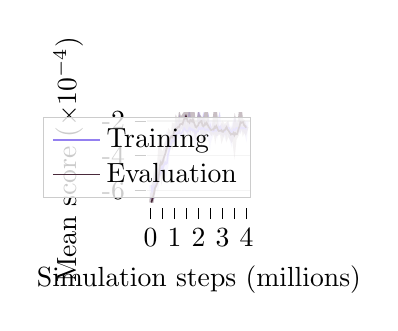
\begin{tikzpicture}

% \begin{axis}[
% axis background/.style={fill=white!82.7450980392157!black},
% axis line style={white},
% legend cell align={left},
% legend style={fill opacity=0.8, draw opacity=1, text opacity=1, at={(1,0.1)}, anchor=south east, draw=white!80!black},
% tick align=outside,
% tick pos=left,
% x grid style={white!69.0196078431373!black},
% xlabel={Simulation steps},
% xmajorgrids,
% xmin=-162030, xmax=4193970,
% xtick style={color=black},
% xtick={-500000,0,500000,1000000,1500000,2000000,2500000,3000000,3500000,4000000,4500000},
% xticklabels={-0.5M,0.0M,0.5M,1.0M,1.5M,2.0M,2.5M,3.0M,3.5M,4.0M,4.5M},
% y grid style={white!69.0196078431373!black},
% ylabel={Mean score},
% ymajorgrids,
% ymin=-7000, ymax=-1500,
% ytick style={color=black}
% ]
\definecolor{color0}{rgb}{0.83921568627451,0.152941176470588,0.156862745098039}
\definecolor{color1}{rgb}{0.12156862745098,0.966666666666667,0.205882352941177}
\definecolor{color2}{rgb}{0.580392156862745,0.503921568627451,0.941176470588235}
\definecolor{color3}{rgb}{0.290196078431372,0.166666666666667,0.23078431372549}

\begin{axis}[
    width=\figurewidth,
    height=\figureheight,
    axis background/.style={fill=white},
    axis line style={white},
    legend cell align={left},
    legend style={fill opacity=0.8, draw opacity=1, text opacity=1, at={(1,0.1)}, anchor=south east, draw=white!80!black},
    tick align=outside,
    tick pos=left,
    x grid style={white},
    xlabel={Simulation steps (millions)},
    xmajorgrids,
    xmin=-162030, 
    xmax=4193970,
    xtick style={color=black},
    xtick={-500000,0,500000,1000000,1500000,2000000,2500000,3000000,3500000,4000000,4500000},
    xticklabels={,0,,1,,2,,3,,4,},
    y grid style={white!80!black},
    ylabel={Mean score ($\times10^{-4}$)},
    ymajorgrids,
    ymin=-7000, 
    ymax=-1500,
    ytick={-10000,-8000,-6000,-4000,-2000},
    yticklabels={-10,-8,-6,-4,-2},
    ytick style={color=black},
    scaled y ticks = false,
    scaled x ticks = false
]
\addplot [ultra thick, color2, opacity=0.3, forget plot]
table {%
35970 -5717.9658203125
71970 -6527.7197265625
107970 -5710.10693359375
143970 -5590.13525390625
179970 -5667.93603515625
215970 -5477.28759765625
251970 -5249.71826171875
287970 -5455.59521484375
323970 -5151.732421875
359970 -4914.23193359375
395970 -4940.73486328125
431970 -4734.75341796875
467970 -4236.5986328125
503970 -4862.49267578125
539970 -4428.56982421875
575970 -4345.30126953125
611970 -4221.07470703125
647970 -4622.47412109375
683970 -4347.73193359375
719970 -3325.75561523438
755970 -3499.94677734375
791970 -3406.83618164062
827970 -3041.74584960938
863970 -2998.71362304688
899970 -2944.29663085938
935970 -3179.16943359375
971970 -3201.15063476562
1007970 -2680.78393554688
1043970 -2683.05712890625
1079970 -2493.4677734375
1115970 -2701.7412109375
1151970 -2700.35717773438
1187970 -2436.07592773438
1223970 -2852.67016601562
1259970 -2833.64526367188
1295970 -2617.94970703125
1331970 -2460.80053710938
1367970 -2423.41772460938
1403970 -2236.19262695312
1439970 -2560.19091796875
1475970 -2679.89086914062
1511970 -2681.22216796875
1547970 -2525.71142578125
1583970 -2526.21044921875
1619970 -2122.64013671875
1655970 -2456.21435546875
1691970 -2659.89990234375
1727970 -2424.8271484375
1763970 -2673.1318359375
1799970 -2435.55224609375
1835970 -2638.96533203125
1871970 -2894.52319335938
1907970 -2572.91088867188
1943970 -2543.2734375
1979970 -2575.82348632812
2015970 -2083.85693359375
2051970 -2565.90966796875
2087970 -2490.20092773438
2123970 -2312.95263671875
2159970 -2493.10668945312
2195970 -2219.71044921875
2231970 -2534.76123046875
2267970 -2657.39184570312
2303970 -2505.4375
2339970 -2438.04858398438
2375970 -2599.87548828125
2411970 -2293.65405273438
2447970 -2603.7470703125
2483970 -1956.734375
2519970 -2808.02514648438
2555970 -2657.88134765625
2591970 -2663.13256835938
2627970 -2626.57495117188
2663970 -2391.04565429688
2699970 -2522.55493164062
2735970 -2631.59814453125
2771970 -2380.25146484375
2807970 -2382.3203125
2843970 -2181.24658203125
2879970 -2738.96704101562
2915970 -2166.55908203125
2951970 -2623.14892578125
2987970 -2675.85864257812
3023970 -2491.10693359375
3059970 -2566.08935546875
3095970 -2679.09887695312
3131970 -2349.10668945312
3167970 -2355.5400390625
3203970 -2468.14013671875
3239970 -2334.83837890625
3275970 -2424.52294921875
3311970 -2756.02124023438
3347970 -2924.38525390625
3383970 -2526.09399414062
3419970 -2490.97241210938
3455970 -2322.40966796875
3491970 -2621.28125
3527970 -2504.16455078125
3563970 -2245.97924804688
3599970 -2392.48803710938
3635970 -2494.2978515625
3671970 -2462.47485351562
3707970 -2511.86010742188
3743970 -2245.16162109375
3779970 -2346.8544921875
3815970 -2463.86376953125
3851970 -2491.453125
3887970 -2344.17407226562
3923970 -2335.02099609375
3959970 -2520.03002929688
3995970 -2009.64904785156
};
\addplot [ultra thick, color3, opacity=0.3, forget plot]
table {%
35970 -6719.6083984375
71970 -6236.591796875
107970 -6182.20458984375
143970 -5896.4560546875
179970 -5466.318359375
215970 -5641.85107421875
251970 -5532.64111328125
287970 -5337.7490234375
323970 -4977.8935546875
359970 -4593.2890625
395970 -3848.08935546875
431970 -4143.34326171875
467970 -4646.28076171875
503970 -4278.3974609375
539970 -3828.50952148438
575970 -3819.96166992188
611970 -3730.05590820312
647970 -3365.81201171875
683970 -3280.53515625
719970 -3354.62866210938
755970 -3012.92919921875
791970 -2717.02221679688
827970 -2781.72216796875
863970 -2803.5810546875
899970 -3052.96166992188
935970 -2803.65551757812
971970 -2279.17553710938
1007970 -2303.54321289062
1043970 -2579.13061523438
1079970 -2238.98852539062
1115970 -2420.93481445312
1151970 -2219.39819335938
1187970 -2345.7109375
1223970 -1985.31372070312
1259970 -2158.07006835938
1295970 -2112.80126953125
1331970 -2249.98291015625
1367970 -1747.04968261719
1403970 -1673.68981933594
1439970 -1866.26220703125
1475970 -1528.25720214844
1511970 -2053.78515625
1547970 -2272.56420898438
1583970 -2022.50390625
1619970 -2198.50805664062
1655970 -1704.84375
1691970 -1978.10681152344
1727970 -2133.98071289062
1763970 -1751.22155761719
1799970 -2273.5361328125
1835970 -2363.53686523438
1871970 -2580.07104492188
1907970 -2415.60986328125
1943970 -2188.39379882812
1979970 -2201.48608398438
2015970 -1901.93212890625
2051970 -2054.44360351562
2087970 -1908.13024902344
2123970 -1977.82189941406
2159970 -2625.55249023438
2195970 -2399.85913085938
2231970 -2178.65014648438
2267970 -1944.18920898438
2303970 -2293.8154296875
2339970 -1971.82397460938
2375970 -2355.0458984375
2411970 -2502.90576171875
2447970 -2489.39379882812
2483970 -2568.86791992188
2519970 -2630.26440429688
2555970 -2490.18701171875
2591970 -2427.63916015625
2627970 -2540.85205078125
2663970 -2094.72729492188
2699970 -2460.74536132812
2735970 -2138.56079101562
2771970 -2539.52807617188
2807970 -2706.23461914062
2843970 -2684.91674804688
2879970 -2533.27075195312
2915970 -2583.59130859375
2951970 -2453.10791015625
2987970 -2783.49926757812
3023970 -2633.94311523438
3059970 -2398.47241210938
3095970 -2494.85302734375
3131970 -2277.875
3167970 -2233.85888671875
3203970 -2726.90625
3239970 -2605.62353515625
3275970 -2764.27905273438
3311970 -2812.78784179688
3347970 -2914.06201171875
3383970 -2692.91186523438
3419970 -2786.08911132812
3455970 -2578.9052734375
3491970 -3022.43408203125
3527970 -2534.83203125
3563970 -2850.97045898438
3599970 -2762.17236328125
3635970 -2391.58154296875
3671970 -2150.82299804688
3707970 -2113.83203125
3743970 -1729.28625488281
3779970 -2156.58569335938
3815970 -2014.46923828125
3851970 -2051.8642578125
3887970 -2450.95776367188
3923970 -2342.0302734375
3959970 -2480.98950195312
3995970 -2315.67651367188
};
\addplot [semithick, color2]
table {%
35970 -5717.9658203125
71970 -6041.8673828125
107970 -5909.163203125
143970 -5781.5520234375
179970 -5736.105628125
215970 -5632.5784159375
251970 -5479.43435425
287970 -5469.8986984875
323970 -5342.6321878425
359970 -5171.272086143
395970 -5079.0571969983
431970 -4941.33568538648
467970 -4659.44086435689
503970 -4740.66158892663
539970 -4615.82488304348
575970 -4507.61543763859
611970 -4392.99914539565
647970 -4484.78913567489
683970 -4429.96625484243
719970 -3988.28199899921
755970 -3792.94791033703
791970 -3638.50321885847
827970 -3399.80027115883
863970 -3239.36561191405
899970 -3121.33801949218
935970 -3144.47058513281
971970 -3167.14260498593
1007970 -2972.59913721031
1043970 -2856.78233388869
1079970 -2711.45650970821
1115970 -2707.57039019993
1151970 -2704.68510521371
1187970 -2597.24143422197
1223970 -2699.41292693943
1259970 -2753.10586163241
1295970 -2699.04339979195
1331970 -2603.74625471892
1367970 -2531.6148426751
1403970 -2413.44595638631
1439970 -2472.14394101929
1475970 -2555.24271226782
1511970 -2605.63449454819
1547970 -2573.66526704142
1583970 -2554.68333991235
1619970 -2381.86605863491
1655970 -2411.60537736845
1691970 -2510.92318735857
1727970 -2476.48477179014
1763970 -2555.14359744908
1799970 -2507.30705690695
1835970 -2559.97036695667
1871970 -2693.79149751775
1907970 -2645.4392539794
1943970 -2604.57292738764
1979970 -2593.07315096383
2015970 -2389.3866640158
2051970 -2459.99586559698
2087970 -2472.07789045194
2123970 -2408.42778895866
2159970 -2442.29934915645
2195970 -2353.26378918137
2231970 -2425.86276569632
2267970 -2518.47439769904
2303970 -2513.25963861943
2339970 -2483.17521676541
2375970 -2529.85532537174
2411970 -2435.3748163168
2447970 -2502.72371791508
2483970 -2284.32798074905
2519970 -2493.80684704318
2555970 -2559.43664728841
2591970 -2600.91501571679
2627970 -2611.17898989883
2663970 -2523.12565565805
2699970 -2522.89736605108
2735970 -2566.37767744315
2771970 -2491.92719240339
2807970 -2448.08444044203
2843970 -2341.34929707772
2879970 -2500.39639465288
2915970 -2366.86146960423
2951970 -2469.37645207504
2987970 -2551.96932827627
3023970 -2527.62437040326
3059970 -2543.01036442946
3095970 -2597.44576943892
3131970 -2498.11013744461
3167970 -2441.08209809176
3203970 -2451.90531354256
3239970 -2405.07853968803
3275970 -2412.85630350032
3311970 -2550.12227819394
3347970 -2699.82746847887
3383970 -2630.33407874357
3419970 -2574.58941208989
3455970 -2473.71751444144
3491970 -2532.74300866486
3527970 -2521.31162551142
3563970 -2411.1786745256
3599970 -2403.70241955911
3635970 -2439.94059236047
3671970 -2448.95429682253
3707970 -2474.11662106227
3743970 -2382.53462107486
3779970 -2368.26256951992
3815970 -2406.50304952445
3851970 -2440.48307971467
3887970 -2401.95947673505
3923970 -2375.18408447853
3959970 -2433.12246240587
3995970 -2263.73309658415
};
\addlegendentry{Training}
\addplot [semithick, color3]
table {%
35970 -6719.6083984375
71970 -6526.4017578125
107970 -6388.722890625
143970 -6191.81615625
179970 -5901.6170375
215970 -5797.7106521875
251970 -5691.682836625
287970 -5550.10931135
323970 -5321.223008685
359970 -5030.049430211
395970 -4557.2654003141
431970 -4391.69654487596
467970 -4493.53023161308
503970 -4407.47712334285
539970 -4175.89008259946
575970 -4033.51871752842
611970 -3912.1335937983
647970 -3693.60496096648
683970 -3528.37703907989
719970 -3458.87768829168
755970 -3280.49829266251
791970 -3055.10786231626
827970 -2945.75358457725
863970 -2888.88457262135
899970 -2954.51541154156
935970 -2894.17145395619
971970 -2648.17308721746
1007970 -2510.32113748673
1043970 -2537.84492858579
1079970 -2418.30236730772
1115970 -2419.35534616588
1151970 -2339.37248504328
1187970 -2341.90786602597
1223970 -2199.27020789683
1259970 -2182.79015208185
1295970 -2154.79459906161
1331970 -2192.86992349947
1367970 -2014.54182714655
1403970 -1878.20102402231
1439970 -1873.42549722588
1475970 -1735.35817919491
1511970 -1862.72897001694
1547970 -2026.66306560392
1583970 -2024.99940186235
1619970 -2094.40286377366
1655970 -1938.5792182642
1691970 -1954.39025556789
1727970 -2026.22643849699
1763970 -1916.22448614507
1799970 -2059.14914481204
1835970 -2180.90423298097
1871970 -2340.57095775733
1907970 -2370.5865199669
1943970 -2297.70943151139
1979970 -2259.22009250058
2015970 -2116.30490706285
2051970 -2091.56038564396
2087970 -2018.18833099575
2123970 -2002.04175836308
2159970 -2251.4460511116
2195970 -2310.81128301071
2231970 -2257.94682840017
2267970 -2132.44378063385
2303970 -2196.99244025531
2339970 -2106.92505399694
2375970 -2206.17339177316
2411970 -2324.8663397514
2447970 -2390.67732338209
2483970 -2461.953561998
2519970 -2529.27789891755
2555970 -2513.64154403803
2591970 -2479.24059048532
2627970 -2503.88517460369
2663970 -2340.22202273096
2699970 -2388.43135816983
2735970 -2288.48313130815
2771970 -2388.90110925364
2807970 -2515.83451320843
2843970 -2583.46740714381
2879970 -2563.38874506754
2915970 -2571.46977047802
2951970 -2524.12502634931
2987970 -2627.87472284084
3023970 -2630.30207979825
3059970 -2537.5702127227
3095970 -2520.48333857112
3131970 -2423.44000314267
3167970 -2347.6075565731
3203970 -2499.32703394386
3239970 -2541.84563442882
3275970 -2630.81900175104
3311970 -2703.60653776937
3347970 -2787.78872734912
3383970 -2749.83798250322
3419970 -2764.33843403318
3455970 -2690.16516979491
3491970 -2823.07273468945
3527970 -2707.77645331367
3563970 -2765.05405558195
3599970 -2763.90137866167
3635970 -2614.9734443845
3671970 -2429.31326584945
3707970 -2303.12077200967
3743970 -2073.58696515893
3779970 -2106.78645643911
3815970 -2069.85956917596
3851970 -2062.66144463058
3887970 -2217.9799722471
3923970 -2267.60009272326
3959970 -2352.9558564152
3995970 -2338.04411931787
};
\addlegendentry{Evaluation}
\end{axis}

\end{tikzpicture}
}
        \caption{IF15 - Large perturbations}
        \label{fig:IF15BigNoise}
    \end{subfigure}
    \begin{subfigure}[t]{0.48\textwidth}
        \centering
        \setlength{\figureheight}{0.5\textwidth}
        \setlength{\figurewidth}{\textwidth}
        \footnotesize{% This file was created by tikzplotlib v0.9.1.
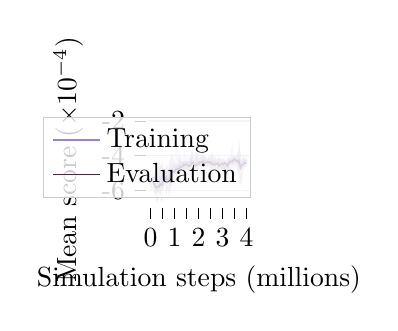
\begin{tikzpicture}

% \begin{axis}[
% axis background/.style={fill=white!82.7450980392157!black},
% axis line style={white},
% legend cell align={left},
% legend style={fill opacity=0.8, draw opacity=1, text opacity=1, at={(1,0.1)}, anchor=south east, draw=white!80!black},
% tick align=outside,
% tick pos=left,
% x grid style={white!69.0196078431373!black},
% xlabel={Simulation steps},
% xmajorgrids,
% xmin=-162030, xmax=4193970,
% xtick style={color=black},
% xtick={-500000,0,500000,1000000,1500000,2000000,2500000,3000000,3500000,4000000,4500000},
% xticklabels={-0.5M,0.0M,0.5M,1.0M,1.5M,2.0M,2.5M,3.0M,3.5M,4.0M,4.5M},
% y grid style={white!69.0196078431373!black},
% ylabel={Mean score},
% ymajorgrids,
% ymin=-7000, ymax=-1500,
% ytick style={color=black}
% ]
\definecolor{color0}{rgb}{0.83921568627451,0.152941176470588,0.156862745098039}
\definecolor{color1}{rgb}{0.12156862745098,0.966666666666667,0.205882352941177}
\definecolor{color2}{rgb}{0.580392156862745,0.503921568627451,0.941176470588235}
\definecolor{color3}{rgb}{0.290196078431372,0.166666666666667,0.23078431372549}

\begin{axis}[
    width=\figurewidth,
    height=\figureheight,
    axis background/.style={fill=white},
    axis line style={white},
    legend cell align={left},
    legend style={fill opacity=0.8, draw opacity=1, text opacity=1, at={(1,0.1)}, anchor=south east, draw=white!80!black},
    tick align=outside,
    tick pos=left,
    x grid style={white},
    xlabel={Simulation steps (millions)},
    xmajorgrids,
    xmin=-162030, 
    xmax=4193970,
    xtick style={color=black},
    xtick={-500000,0,500000,1000000,1500000,2000000,2500000,3000000,3500000,4000000,4500000},
    xticklabels={,0,,1,,2,,3,,4,},
    y grid style={white!80!black},
    ylabel={Mean score ($\times10^{-4}$)},
    ymajorgrids,
    ymin=-7000, 
    ymax=-1500,
    ytick={-10000,-8000,-6000,-4000,-2000},
    yticklabels={-10,-8,-6,-4,-2},
    ytick style={color=black},
    scaled y ticks = false,
    scaled x ticks = false
]
\addplot [ultra thick, color2, opacity=0.3, forget plot]
table {%
35970 -5317.88427734375
71970 -5322.189453125
107970 -5166.73779296875
143970 -5243.4833984375
179970 -5465.33447265625
215970 -5349.076171875
251970 -5393.81689453125
287970 -5832.51513671875
323970 -5530.68505859375
359970 -5274.5556640625
395970 -5000.19677734375
431970 -5164.30126953125
467970 -5587.755859375
503970 -5116.3046875
539970 -5256.17724609375
575970 -5334.36376953125
611970 -5237.8564453125
647970 -5280.3623046875
683970 -5191.02001953125
719970 -5208.501953125
755970 -4865.50048828125
791970 -4861.365234375
827970 -5222.595703125
863970 -4929.623046875
899970 -4836.81005859375
935970 -4856.666015625
971970 -4618.90673828125
1007970 -4546.20556640625
1043970 -4834.41064453125
1079970 -4329.8720703125
1115970 -4614.42236328125
1151970 -4683.42724609375
1187970 -4683.265625
1223970 -4319.74072265625
1259970 -4492.78125
1295970 -4390.68310546875
1331970 -4548.16064453125
1367970 -4438.8828125
1403970 -4637.29052734375
1439970 -4273.55224609375
1475970 -4398.58544921875
1511970 -4354.76904296875
1547970 -4335.16064453125
1583970 -4567.82470703125
1619970 -4255.0439453125
1655970 -4285.923828125
1691970 -4249.2529296875
1727970 -4500.4755859375
1763970 -4438.94091796875
1799970 -4457.521484375
1835970 -4430.2685546875
1871970 -4476.62841796875
1907970 -4429.2021484375
1943970 -4213.060546875
1979970 -4466.50830078125
2015970 -4474.875
2051970 -4700.68115234375
2087970 -4457.14794921875
2123970 -4414.57470703125
2159970 -4114.77490234375
2195970 -4376.7470703125
2231970 -4297.4892578125
2267970 -4220.42578125
2303970 -4382.79736328125
2339970 -4367.68896484375
2375970 -4439.00244140625
2411970 -4334.408203125
2447970 -4458.15966796875
2483970 -4488.705078125
2519970 -4509.79150390625
2555970 -4512.84716796875
2591970 -4178.8544921875
2627970 -4277.28759765625
2663970 -4400.17333984375
2699970 -4420.748046875
2735970 -4545.38916015625
2771970 -4553.6162109375
2807970 -4407.14697265625
2843970 -4614.2509765625
2879970 -4638.0546875
2915970 -4385.4111328125
2951970 -4422.05615234375
2987970 -4464.23095703125
3023970 -4715.94873046875
3059970 -4718.810546875
3095970 -4532.19775390625
3131970 -4568.50830078125
3167970 -4639.21337890625
3203970 -4550.330078125
3239970 -4575.10791015625
3275970 -4362.6669921875
3311970 -4406.0244140625
3347970 -4444.88916015625
3383970 -4177.29833984375
3419970 -4706.60595703125
3455970 -4441.75830078125
3491970 -4224.486328125
3527970 -4233.181640625
3563970 -4356.1455078125
3599970 -4241.8544921875
3635970 -4146.5732421875
3671970 -4518.146484375
3707970 -4431.8623046875
3743970 -4593.89892578125
3779970 -4625.33740234375
3815970 -4572.86083984375
3851970 -4346.36279296875
3887970 -4130.1796875
3923970 -4144.62060546875
3959970 -4317.59716796875
3995970 -4326.37939453125
};
\addplot [ultra thick, color3, opacity=0.3, forget plot]
table {%
35970 -5325.0419921875
71970 -5680.65966796875
107970 -5603.9970703125
143970 -5758.970703125
179970 -5859.8154296875
215970 -6011.02490234375
251970 -5942.39501953125
287970 -5706.1689453125
323970 -5732.15283203125
359970 -5843.3662109375
395970 -5377.7578125
431970 -5784.9111328125
467970 -5722.19970703125
503970 -5225.3017578125
539970 -5509.22412109375
575970 -5350.767578125
611970 -5249.31396484375
647970 -5085.8017578125
683970 -5558.328125
719970 -5355.64501953125
755970 -5577.04541015625
791970 -5105.9677734375
827970 -4789.74169921875
863970 -5046.40185546875
899970 -4677.76416015625
935970 -5010.1279296875
971970 -4967.7265625
1007970 -4904.80224609375
1043970 -4633.32177734375
1079970 -4668.21044921875
1115970 -4839.72509765625
1151970 -4711.705078125
1187970 -4779.884765625
1223970 -4501.14892578125
1259970 -4609.9443359375
1295970 -4660.8193359375
1331970 -4603.5537109375
1367970 -4462.0830078125
1403970 -4472.4013671875
1439970 -4610.0927734375
1475970 -4458.1591796875
1511970 -4492.3369140625
1547970 -4624.3212890625
1583970 -4696.986328125
1619970 -4610.6904296875
1655970 -4467.15869140625
1691970 -4485.20556640625
1727970 -4230.00634765625
1763970 -4495.1513671875
1799970 -4506.53759765625
1835970 -4713.57373046875
1871970 -4661.1357421875
1907970 -4371.80322265625
1943970 -4569.5205078125
1979970 -4480.8115234375
2015970 -4341.822265625
2051970 -4281.5126953125
2087970 -4392.9404296875
2123970 -4371.900390625
2159970 -4246.853515625
2195970 -4466.376953125
2231970 -4445.162109375
2267970 -4347.5107421875
2303970 -4465.78564453125
2339970 -4352.45458984375
2375970 -4377.1904296875
2411970 -4433.83544921875
2447970 -4306.4599609375
2483970 -4388.02099609375
2519970 -4610.41748046875
2555970 -4399.7646484375
2591970 -4628.35986328125
2627970 -4570.16748046875
2663970 -4510.79443359375
2699970 -4386.10107421875
2735970 -4507.65673828125
2771970 -4448.294921875
2807970 -4394.4423828125
2843970 -4834.21240234375
2879970 -4525.52001953125
2915970 -4455.44775390625
2951970 -4375.07861328125
2987970 -4446.81396484375
3023970 -4603.95166015625
3059970 -4352.4208984375
3095970 -4380.45458984375
3131970 -4600.70361328125
3167970 -4516.0185546875
3203970 -4719.4130859375
3239970 -4317.68505859375
3275970 -4251.4130859375
3311970 -4255.07958984375
3347970 -4370.4541015625
3383970 -4348.2197265625
3419970 -4245.951171875
3455970 -4165.0380859375
3491970 -4154.58837890625
3527970 -4329.4443359375
3563970 -4346.52099609375
3599970 -4347.228515625
3635970 -4462.75830078125
3671970 -4179.27099609375
3707970 -4781.92138671875
3743970 -5000.4541015625
3779970 -4436.72607421875
3815970 -4447.30517578125
3851970 -4512.71875
3887970 -4336.515625
3923970 -4361.78662109375
3959970 -4489.162109375
3995970 -4449.84619140625
};
\addplot [semithick, color2]
table {%
35970 -5317.88427734375
71970 -5319.60634765625
107970 -5258.45892578125
143970 -5252.46871484375
179970 -5337.61501796875
215970 -5342.19947953125
251970 -5362.84644553125
287970 -5550.71392200625
323970 -5542.70237664125
359970 -5435.44369160975
395970 -5261.34492590335
431970 -5222.52746335451
467970 -5368.61882176271
503970 -5267.69316805762
539970 -5263.08679927207
575970 -5291.59758737574
611970 -5270.10113055045
647970 -5274.20560020527
683970 -5240.93136793566
719970 -5227.9596020114
755970 -5082.97595651934
791970 -4994.3316676616
827970 -5085.63728184696
863970 -5023.23158785818
899970 -4948.66297615241
935970 -4911.86419194144
971970 -4794.68121047737
1007970 -4695.29095284892
1043970 -4750.93882952185
1079970 -4582.51212583811
1115970 -4595.27622081537
1151970 -4630.53663092672
1187970 -4651.62822855603
1223970 -4518.87322619612
1259970 -4508.43643571767
1295970 -4461.3351036181
1331970 -4496.06531998336
1367970 -4473.19231699002
1403970 -4538.83160113151
1439970 -4432.71985911641
1475970 -4419.06609515734
1511970 -4393.34727428191
1547970 -4370.07262238164
1583970 -4449.17345624149
1619970 -4371.52165186989
1655970 -4337.28252237193
1691970 -4302.07068529816
1727970 -4381.4326455539
1763970 -4404.43595451984
1799970 -4425.6701664619
1835970 -4427.50952175214
1871970 -4447.15708023879
1907970 -4439.97510751827
1943970 -4349.20928326096
1979970 -4396.12889026908
2015970 -4427.62733416145
2051970 -4536.84886143437
2087970 -4504.96849654812
2123970 -4468.81098074137
2159970 -4327.19654938232
2195970 -4347.01675775439
2231970 -4327.20575777764
2267970 -4284.49376716658
2303970 -4323.81520561245
2339970 -4341.36470930497
2375970 -4380.41980214548
2411970 -4362.01516253729
2447970 -4400.47296470987
2483970 -4435.76581007592
2519970 -4465.37608760805
2555970 -4484.36451975233
2591970 -4362.1605087264
2627970 -4328.21134429834
2663970 -4356.9961425165
2699970 -4382.4969042599
2735970 -4447.65380661844
2771970 -4490.03876834606
2807970 -4456.88205007014
2843970 -4519.82962066708
2879970 -4567.11964740025
2915970 -4494.43624156515
2951970 -4465.48420587659
2987970 -4464.98290633845
3023970 -4565.36923599057
3059970 -4626.74576034434
3095970 -4588.92655776911
3131970 -4580.75925497396
3167970 -4604.14090454688
3203970 -4582.61657397813
3239970 -4579.61310844938
3275970 -4492.83466194463
3311970 -4458.11056279178
3347970 -4452.82200173757
3383970 -4342.61253698004
3419970 -4488.20990500052
3455970 -4469.62926331281
3491970 -4371.57208923769
3527970 -4316.21590979261
3563970 -4332.18774900057
3599970 -4296.05444627534
3635970 -4236.2619646402
3671970 -4349.01577253412
3707970 -4382.15438539547
3743970 -4466.85220154978
3779970 -4530.24628186737
3815970 -4547.29210505792
3851970 -4466.92038022225
3887970 -4332.22410313335
3923970 -4257.18270406751
3959970 -4281.34848962801
3995970 -4299.3608515893
};
\addlegendentry{Training}
\addplot [semithick, color3]
table {%
35970 -5325.0419921875
71970 -5467.2890625
107970 -5521.972265625
143970 -5616.771640625
179970 -5713.98915625
215970 -5832.8034546875
251970 -5876.640080625
287970 -5808.4516265
323970 -5777.9321087125
359970 -5804.1057496025
395970 -5633.5665747615
431970 -5694.1043979819
467970 -5705.34252160164
503970 -5513.32621608598
539970 -5511.68537808909
575970 -5447.31825810345
611970 -5368.11654079957
647970 -5255.19062760474
683970 -5376.44562656285
719970 -5368.12538375021
755970 -5451.69339431263
791970 -5313.40314596257
827970 -5103.93856726505
863970 -5080.92388254653
899970 -4919.65999359042
935970 -4955.84716802925
971970 -4960.59892581755
1007970 -4938.28025392803
1043970 -4816.29686329432
1079970 -4757.06229766409
1115970 -4790.12741766095
1151970 -4758.75848184657
1187970 -4767.20899535794
1223970 -4660.78496752727
1259970 -4640.44871489136
1295970 -4648.59696330982
1331970 -4630.57966236089
1367970 -4563.18100054153
1403970 -4526.86914719992
1439970 -4560.15859769495
1475970 -4519.35883049197
1511970 -4508.55006392018
1547970 -4554.85855397711
1583970 -4611.70966363626
1619970 -4611.30197005676
1655970 -4553.64465859656
1691970 -4526.26902172043
1727970 -4407.76395209476
1763970 -4442.71891813186
1799970 -4468.24638994161
1835970 -4566.37732615247
1871970 -4604.28069256648
1907970 -4511.28970460239
1943970 -4534.58202588643
1979970 -4513.07382490686
2015970 -4444.57320119412
2051970 -4379.34899884147
2087970 -4384.78557117988
2123970 -4379.63149895793
2159970 -4326.52030562476
2195970 -4382.46296462485
2231970 -4407.54262252491
2267970 -4383.52987038995
2303970 -4416.43218004647
2339970 -4390.84114396538
2375970 -4385.38085825423
2411970 -4404.76269464004
2447970 -4365.44160115902
2483970 -4374.47335913291
2519970 -4468.85100766725
2555970 -4441.21646397535
2591970 -4516.07382369771
2627970 -4537.71128640613
2663970 -4526.94454528118
2699970 -4470.60715685621
2735970 -4485.42698942622
2771970 -4470.57416240573
2807970 -4440.12145056844
2843970 -4597.75783127856
2879970 -4568.86270657964
2915970 -4523.49672551028
2951970 -4464.12948061867
2987970 -4457.2032743087
3023970 -4515.90262864772
3059970 -4450.50993656363
3095970 -4422.48779787568
3131970 -4493.77412403791
3167970 -4502.67189629774
3203970 -4589.36837215365
3239970 -4480.69504672969
3275970 -4388.98226241281
3311970 -4335.42119338519
3347970 -4349.43435665611
3383970 -4348.94850461867
3419970 -4307.7495715212
3455970 -4250.66497728772
3491970 -4212.23433793513
3527970 -4259.11833713608
3563970 -4294.07940071915
3599970 -4315.33904668149
3635970 -4374.30674832139
3671970 -4296.29244743034
3707970 -4490.5440231457
3743970 -4694.50805451242
3779970 -4591.39526239495
3815970 -4533.75922774947
3851970 -4525.34303664968
3887970 -4449.81207198981
3923970 -4414.60189163139
3959970 -4444.42597872883
3995970 -4446.5940637998
};
\addlegendentry{Evaluation}
\end{axis}

\end{tikzpicture}
}
        \caption{OF15 - Large perturbations}
        \label{fig:OF15BigNoise}
    \end{subfigure}
    \begin{subfigure}[t]{0.48\textwidth}
        \centering
        \setlength{\figureheight}{0.5\textwidth}
        \setlength{\figurewidth}{\textwidth}
        \footnotesize{\input{fig_latex_v2/20200629T101439}}
        \caption{OF25 - Each agent exposed to a different environment}
        \label{fig:OFMN25}
    \end{subfigure}
    \begin{subfigure}[t]{0.48\textwidth}
        \centering
        \setlength{\figureheight}{0.5\textwidth}
        \setlength{\figurewidth}{\textwidth}
        \footnotesize{% This file was created by tikzplotlib v0.9.1.
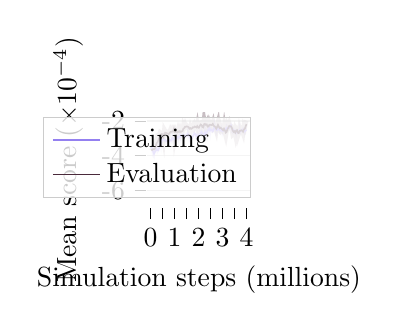
\begin{tikzpicture}

% \begin{axis}[
% axis background/.style={fill=white!82.7450980392157!black},
% axis line style={white},
% legend cell align={left},
% legend style={fill opacity=0.8, draw opacity=1, text opacity=1, at={(1,0.1)}, anchor=south east, draw=white!80!black},
% tick align=outside,
% tick pos=left,
% x grid style={white!69.0196078431373!black},
% xlabel={Timestep},
% xmajorgrids,
% xmin=-162030, xmax=4193970,
% xtick style={color=black},
% xtick={-500000,0,500000,1000000,1500000,2000000,2500000,3000000,3500000,4000000,4500000},
% xticklabels={-0.5M,0.0M,0.5M,1.0M,1.5M,2.0M,2.5M,3.0M,3.5M,4.0M,4.5M},
% y grid style={white!69.0196078431373!black},
% ylabel={Mean score},
% ymajorgrids,
% ymin=-10500, ymax=-1500,
% ytick style={color=black}
% ]
\definecolor{color0}{rgb}{0.83921568627451,0.152941176470588,0.156862745098039}
\definecolor{color1}{rgb}{0.12156862745098,0.966666666666667,0.205882352941177}
\definecolor{color2}{rgb}{0.580392156862745,0.503921568627451,0.941176470588235}
\definecolor{color3}{rgb}{0.290196078431372,0.166666666666667,0.23078431372549}

\begin{axis}[
    width=\figurewidth,
    height=\figureheight,
    axis background/.style={fill=white},
    axis line style={white},
    legend cell align={left},
    legend style={fill opacity=0.8, draw opacity=1, text opacity=1, at={(1,0.1)}, anchor=south east, draw=white!80!black},
    tick align=outside,
    tick pos=left,
    x grid style={white},
    xlabel={Simulation steps (millions)},
    xmajorgrids,
    xmin=-162030, 
    xmax=4193970,
    xtick style={color=black},
    xtick={-500000,0,500000,1000000,1500000,2000000,2500000,3000000,3500000,4000000,4500000},
    xticklabels={,0,,1,,2,,3,,4,},
    y grid style={white!80!black},
    ylabel={Mean score ($\times10^{-4}$)},
    ymajorgrids,
    ymin=-7000, 
    ymax=-1500,
    ytick={-10000,-8000,-6000,-4000,-2000},
    yticklabels={-10,-8,-6,-4,-2},
    ytick style={color=black},
    scaled y ticks = false,
    scaled x ticks = false
]

\addplot [semithick, color2, opacity=0.3, forget plot]
table {%
35970 -3488.79174804688
71970 -3756.9609375
107970 -4009.18725585938
143970 -4087.7333984375
179970 -3644.32275390625
215970 -3618.22094726562
251970 -3442.68920898438
287970 -3790.08911132812
323970 -3712.85302734375
359970 -3321.1298828125
395970 -3058.10229492188
431970 -3412.46020507812
467970 -2701.01147460938
503970 -3125.79174804688
539970 -2886.7119140625
575970 -3156.84985351562
611970 -3143.08715820312
647970 -3264.4033203125
683970 -3149.21826171875
719970 -3025.52734375
755970 -3034.17065429688
791970 -3289.21923828125
827970 -3029.56665039062
863970 -3148.62939453125
899970 -2778.93432617188
935970 -3120.1259765625
971970 -2993.88647460938
1007970 -3152.12060546875
1043970 -3015.73315429688
1079970 -2707.37573242188
1115970 -2931.97314453125
1151970 -3103.54541015625
1187970 -2804.5126953125
1223970 -2672.52807617188
1259970 -3039.44848632812
1295970 -2784.25073242188
1331970 -2797.72900390625
1367970 -2736.18823242188
1403970 -3015.41870117188
1439970 -2905.62353515625
1475970 -2762.68139648438
1511970 -2880.66845703125
1547970 -2565.5732421875
1583970 -2834.31225585938
1619970 -3110.17236328125
1655970 -2966.8603515625
1691970 -3140.90502929688
1727970 -2929.96655273438
1763970 -2766.16137695312
1799970 -2653.43188476562
1835970 -2590.20166015625
1871970 -2844.2041015625
1907970 -3027.8916015625
1943970 -2723.28100585938
1979970 -3024.43505859375
2015970 -2809.39111328125
2051970 -2576.89013671875
2087970 -2647.96875
2123970 -2512.15356445312
2159970 -2848.1005859375
2195970 -2854.38330078125
2231970 -2890.13647460938
2267970 -2411.99243164062
2303970 -2920.16625976562
2339970 -2554.49560546875
2375970 -2416.94506835938
2411970 -2355.7724609375
2447970 -2323.28588867188
2483970 -2748.5810546875
2519970 -2420.71508789062
2555970 -2636.26245117188
2591970 -2640.92895507812
2627970 -2381.44848632812
2663970 -2103.77734375
2699970 -2433.71508789062
2735970 -2725.3505859375
2771970 -2560.62280273438
2807970 -2361.5791015625
2843970 -2366.14770507812
2879970 -2654.921875
2915970 -2568.94702148438
2951970 -2411.9755859375
2987970 -2721.9931640625
3023970 -2538.91284179688
3059970 -2486.6494140625
3095970 -2443.58862304688
3131970 -2462.3525390625
3167970 -2278.6884765625
3203970 -2376.73510742188
3239970 -2480.7197265625
3275970 -2381.97094726562
3311970 -2231.43969726562
3347970 -2163.27612304688
3383970 -2635.28637695312
3419970 -2687.94140625
3455970 -2517.92407226562
3491970 -2663.86767578125
3527970 -2575.4619140625
3563970 -2782.81298828125
3599970 -2577.3271484375
3635970 -2716.13745117188
3671970 -2693.06665039062
3707970 -2373.37158203125
3743970 -2661.74243164062
3779970 -2531.13598632812
3815970 -2480.98974609375
3851970 -2416.30688476562
3887970 -2552.51318359375
3923970 -2725.03442382812
3959970 -2480.75659179688
3995970 -2486.65502929688
};
\addplot [ultra thick, color3, opacity=0.3, forget plot]
table {%
35970 -3700.51000976562
71970 -3594.20825195312
107970 -3578.27685546875
143970 -3636.07958984375
179970 -3560.24536132812
215970 -3222.09350585938
251970 -3039.92846679688
287970 -3151.86987304688
323970 -2967.29614257812
359970 -2780.93115234375
395970 -2649.9716796875
431970 -2684.97387695312
467970 -2699.87426757812
503970 -2814.45751953125
539970 -3106.32592773438
575970 -2493.51928710938
611970 -2581.92602539062
647970 -2716.26782226562
683970 -2790.69384765625
719970 -2714.4326171875
755970 -2813.28833007812
791970 -2643.7587890625
827970 -2507.91357421875
863970 -2617.5390625
899970 -2588.63403320312
935970 -2613.93969726562
971970 -2220.83447265625
1007970 -2949.95678710938
1043970 -2641.1787109375
1079970 -2602.89111328125
1115970 -2721.61352539062
1151970 -2510.46948242188
1187970 -2682.98608398438
1223970 -2513.63208007812
1259970 -2702.62768554688
1295970 -2549.05688476562
1331970 -2567.99047851562
1367970 -2238.06884765625
1403970 -2351.63330078125
1439970 -2203.88110351562
1475970 -2338.1474609375
1511970 -2282.5185546875
1547970 -2350.83520507812
1583970 -2403.62939453125
1619970 -2575.66528320312
1655970 -2363.82763671875
1691970 -2521.13647460938
1727970 -2376.95361328125
1763970 -2272.75903320312
1799970 -2397.59643554688
1835970 -2238.15161132812
1871970 -2362.69946289062
1907970 -2417.68310546875
1943970 -2187.7587890625
1979970 -2516.95654296875
2015970 -2403.16235351562
2051970 -2106.41137695312
2087970 -2092.4912109375
2123970 -2269.29077148438
2159970 -2529.74438476562
2195970 -2411.19116210938
2231970 -1898.97790527344
2267970 -2150.56201171875
2303970 -2294.9365234375
2339970 -2163.01245117188
2375970 -2526.9306640625
2411970 -2319.87963867188
2447970 -2073.19799804688
2483970 -2205.49438476562
2519970 -2260.33984375
2555970 -2220.1943359375
2591970 -2080.34033203125
2627970 -2428.74633789062
2663970 -2372.40356445312
2699970 -2403.13549804688
2735970 -2578.64892578125
2771970 -2222.0302734375
2807970 -2045.22521972656
2843970 -2478.66455078125
2879970 -2540.3994140625
2915970 -2337.69165039062
2951970 -2503.51611328125
2987970 -2571.96362304688
3023970 -2620.46069335938
3059970 -2308.46850585938
3095970 -2681.00732421875
3131970 -2873.4873046875
3167970 -2574.96826171875
3203970 -2200.2529296875
3239970 -2292.55444335938
3275970 -2144.57543945312
3311970 -2309.24829101562
3347970 -2310.47680664062
3383970 -2518.61010742188
3419970 -2788.25659179688
3455970 -2738.55517578125
3491970 -2549.07934570312
3527970 -2790.34790039062
3563970 -2413.42553710938
3599970 -2479.17407226562
3635970 -2889.03247070312
3671970 -2734.72924804688
3707970 -2401.47924804688
3743970 -2559.546875
3779970 -2486.7705078125
3815970 -2577.72143554688
3851970 -2722.33862304688
3887970 -2296.82250976562
3923970 -2395.76196289062
3959970 -2106.31420898438
3995970 -1981.36193847656
};
\addplot [semithick, color2]
table {%
35970 -3488.79174804688
71970 -3596.05942382813
107970 -3761.31055664063
143970 -3891.87969335938
179970 -3792.85691757813
215970 -3723.00252945313
251970 -3610.87720126562
287970 -3682.56196529062
323970 -3694.67839011187
359970 -3545.25898719212
395970 -3350.39631028402
431970 -3375.22186820166
467970 -3105.53771076475
503970 -3113.6393256776
539970 -3022.86836103156
575970 -3076.46095802519
611970 -3103.11143809636
647970 -3167.62819098282
683970 -3160.26421927719
719970 -3106.36946906631
755970 -3077.48994315854
791970 -3162.18166120762
827970 -3109.13565688082
863970 -3124.93315194099
899970 -2986.53362163335
935970 -3039.97056360501
971970 -3021.53692800675
1007970 -3073.77039899155
1043970 -3050.55550111368
1079970 -2913.28359363696
1115970 -2920.75941399468
1151970 -2993.87381245931
1187970 -2918.12936560058
1223970 -2819.8888498291
1259970 -2907.71270442871
1295970 -2858.32791562598
1331970 -2834.08835093809
1367970 -2794.9283035316
1403970 -2883.12446258771
1439970 -2892.12409161513
1475970 -2840.34701356283
1511970 -2856.4755909502
1547970 -2740.11465144512
1583970 -2777.79369321082
1619970 -2910.74516123899
1655970 -2933.1912373684
1691970 -3016.27675413979
1727970 -2981.75267357762
1763970 -2895.51615492782
1799970 -2798.68244686294
1835970 -2715.29013218027
1871970 -2766.85571993316
1907970 -2871.2700725849
1943970 -2812.07444589469
1979970 -2897.01869097431
2015970 -2861.96765989709
2051970 -2747.93665062575
2087970 -2707.94949037545
2123970 -2629.63112000652
2159970 -2717.01890637891
2195970 -2771.96466413985
2231970 -2819.23338832766
2267970 -2656.33700565285
2303970 -2761.86870729796
2339970 -2678.91946656627
2375970 -2574.12970728351
2411970 -2486.78680874511
2447970 -2421.38644071582
2483970 -2552.26428630449
2519970 -2499.64460693894
2555970 -2554.29174463212
2591970 -2588.94662881052
2627970 -2505.94737181756
2663970 -2345.07936059054
2699970 -2380.53365151057
2735970 -2518.46042528134
2771970 -2535.32537626256
2807970 -2465.82686638253
2843970 -2425.95520186077
2879970 -2517.54187111646
2915970 -2538.10393126363
2951970 -2487.65259313318
2987970 -2581.38882150491
3023970 -2564.39842962169
3059970 -2533.29882339802
3095970 -2497.41474325756
3131970 -2483.38986157954
3167970 -2401.50930757272
3203970 -2391.59962751238
3239970 -2427.24766713243
3275970 -2409.13697918571
3311970 -2338.05806641767
3347970 -2268.14528906935
3383970 -2415.00172422286
3419970 -2524.17759703372
3455970 -2521.67618712648
3491970 -2578.55278258839
3527970 -2577.31643517803
3563970 -2659.51505641932
3599970 -2626.63989322659
3635970 -2662.43891640471
3671970 -2674.69000999907
3707970 -2554.16263881194
3743970 -2597.19455594342
3779970 -2570.7711280973
3815970 -2534.85857529588
3851970 -2487.43789908378
3887970 -2513.46801288777
3923970 -2598.09457726391
3959970 -2551.1593830771
3995970 -2525.35764156501
};
\addlegendentry{Training}
\addplot [semithick, color3]
table {%
35970 -3700.51000976562
71970 -3657.98930664063
107970 -3626.10432617188
143970 -3630.09443164063
179970 -3602.15480351563
215970 -3450.13028445313
251970 -3286.04955739062
287970 -3232.37768365313
323970 -3126.34506722312
359970 -2988.17950127137
395970 -2852.89637263783
431970 -2785.72737436395
467970 -2751.38613164962
503970 -2776.61468680227
539970 -2908.49918317511
575970 -2742.50722474882
611970 -2678.27474500554
647970 -2693.47197590957
683970 -2732.36072460824
719970 -2725.18948163995
755970 -2760.42902101522
791970 -2713.76092823413
827970 -2631.42198662798
863970 -2625.86881697679
899970 -2610.97490346732
935970 -2612.16082098664
971970 -2455.63028165449
1007970 -2653.36088383644
1043970 -2648.48801467687
1079970 -2630.24925411862
1115970 -2666.79496262742
1151970 -2604.2647705452
1187970 -2635.75329592087
1223970 -2586.90480958377
1259970 -2633.19395996901
1295970 -2599.53912988766
1331970 -2586.91966933884
1367970 -2447.37934066581
1403970 -2409.08092471198
1439970 -2327.00099623344
1475970 -2331.45958211506
1511970 -2311.88317114404
1547970 -2327.46398471767
1583970 -2357.9301486431
1619970 -2445.02420246711
1655970 -2412.54557616777
1691970 -2455.98193554441
1727970 -2424.37060663915
1763970 -2363.72597726474
1799970 -2377.27416057759
1835970 -2321.62514087781
1871970 -2338.05486968293
1907970 -2369.90616399726
1943970 -2297.04721402336
1979970 -2385.01094560151
2015970 -2392.27150876716
2051970 -2277.92745604155
2087970 -2203.75295799993
2123970 -2229.96808339371
2159970 -2349.87860394247
2195970 -2374.40362720923
2231970 -2184.23333843492
2267970 -2170.76480774845
2303970 -2220.43349402407
2339970 -2197.46507688319
2375970 -2329.25131175492
2411970 -2325.5026425217
2447970 -2224.58078473177
2483970 -2216.94622474531
2519970 -2234.30367234719
2555970 -2228.65993778331
2591970 -2169.33209548249
2627970 -2273.09779244574
2663970 -2312.8201012487
2699970 -2348.94625996797
2735970 -2440.82732629328
2771970 -2353.30850515097
2807970 -2230.07519098121
2843970 -2329.51093490122
2879970 -2413.86632656573
2915970 -2383.39645609569
2951970 -2431.44431896991
2987970 -2487.6520406007
3023970 -2540.77550170417
3059970 -2447.85270336625
3095970 -2541.11455170725
3131970 -2674.06365289935
3167970 -2634.42549642711
3203970 -2460.75646973127
3239970 -2393.47565918251
3275970 -2293.91557129076
3311970 -2300.0486591807
3347970 -2304.21991816467
3383970 -2389.97599386755
3419970 -2549.28823303928
3455970 -2624.99501013607
3491970 -2594.62874436289
3527970 -2672.91640677398
3563970 -2569.12005890814
3599970 -2533.14166425113
3635970 -2675.49798683193
3671970 -2699.19049131791
3707970 -2580.1059940095
3743970 -2571.8823464057
3779970 -2537.83761096842
3815970 -2553.7911407998
3851970 -2621.21013369863
3887970 -2491.45508412543
3923970 -2453.17783563151
3959970 -2314.43238497265
3995970 -2181.20420637422
};
\addlegendentry{Evaluation}
\end{axis}

\end{tikzpicture}
}
        \caption{IF25 - Each agent exposed to a different environment}
        \label{fig:IFMN25}
    \end{subfigure}
    \caption{Simulation results with an extra 4 scenarios analyzed: two of them where we consider perturbations of larger magnitude, and two more where we consider that each of the agents in a modified environment is affected differently.}
    \label{fig:more_results}
\end{figure*}

Comparing perturbations in the sensors versus perturbations in the actuators, we see an overall more robust performance against adversarial elements in the sensing part. In Figures~\ref{fig:IF5} to~\ref{fig:IF25}, we see that the network always converges and we only see more unstable behaviour when there is a large fraction of agents suffering of variable sensing errors (50\% and 83\%). When we compare the effect of constant or fixed perturbations against variable ones, we notice that variable perturbations induce less stable convergence. This can be to some extent explained by the fact that there are no large subsets of agents being exposed to a common environment.

For small fixed perturbations affecting actuation (output disturbances), we have seen that the agents are able to converge towards a working policy. In the cases where 5 or 25 of the agents are affected, this was expected as there is a majority (25) of agents, in both cases, that work in exactly the same way, and a small subset (5) that work in a slightly different way (but still the same within that subset). When this fixed perturbation is introduced to half of the agents, then we have two subsets of the same size operating in different ways, but again consistently across each of the subsets. In this case, we have seen that for a small magnitude in the perturbation, the agents still converge on a policy that works for both subsets. As the difference between the operation of the agents in these two subsets diverges, the performance of the system as a whole drops significantly. Nonetheless, we have observed that the case were half of the agents have a common fixed perturbation of small magnitude the system is able to converge even when the initial conditions are disadvantageous. 

In order to analyze the effect of perturbations with larger magnitude as well as fixed perturbations in both sensing and actuation that vary across the robots exposed to a modified environment, we have analyzed four more cases shown in Fig.~\ref{fig:more_results}. In Figures~\ref{fig:IF15BigNoise} and~\ref{fig:OF15BigNoise}, we analyze how perturbations with larger magnitude affect the learning process, with half of the agents being affected as the worst-case scenario. We see that the trend from the previous results is followed, with the network being able to converge to a common policy when a constant error is added to the sensors interface, but not when the disturbances affect to the actuators. Finally, Figures~\ref{fig:OFMN25} and~\ref{fig:IFMN25} show that when there are no differentiated subsets of agents with a common behaviour and the perturbations are different across a large number of agents, then the system is not able to converge.


   

\section{Conclusion and Future Work}\label{sec:conclusion}

Adversarial agents and closing the simulation-to-reality gap are among the key challenges preventing wider adoption of reinforcement learning in real-world applications. In this paper, we have addressed the latter one from the perspective of the former: by introducing adversarial conditions inspired by real-world perturbances to a subset of agents in a multi-robot system during a collaborative reinforcement learning process, we have been able to identify points where the robustness of distributed multi-agent DRL algorithms needs to be improved. In this paper, we have considered multiple robotic arms in a simulation environment collaborating towards learning a common policy to reach an object. In order to emulate more realistic conditions and understand how perturbances in the environment affect the learning process, we have considered variability across the agents in terms of their ability to sense and actuate accurately. We have shown how different types of disturbances in the model's input (sensing) and output (actuation) affect the robustness and ability to converge towards an effective policy. We have seen how variable perturbances have the most effect on the ability of the network to converge, while disturbances in the ability of the robots to actuate properly have had a comparatively worse effect than those in their ability to sense the position of the object accurately.

The conclusions of this work serve as a starting point towards the design and development of more robust methods able to identify and take into account these disturbances in the environment that do not occur across all robots equally. This will be the subject of our future work, as well as the study of other types or combinations of disturbances in the environment. We will also work towards modeling more accurately real-world errors for RL simulation environments.

%%%%%%%%%%%%%%%%%%%%%%%%%%%%%%%%%%%%%%%%%%%%%%
%%                                          %%
%%     ACKNOWLEDGEMENT AND BIBLIOGRAPHY     %%
%%                                          %%
%%%%%%%%%%%%%%%%%%%%%%%%%%%%%%%%%%%%%%%%%%%%%%

\section*{Acknowledgements}

This work was supported by the Academy of Finland's AutoSOS project with grant number 328755.


% \nocite{*}
\bibliographystyle{unsrt}
\bibliography{ref}

% \clearpage
% \newpage
% \Large{\textbf{Authors' Background}} \\[+23pt]
% \normalsize
% \begin{tabular}{@{}llll@{}}
%     \toprule
%     \textbf{Name} & \textbf{Title} & \textbf{Research Field} & \textbf{Personal Website} \\
%     \midrule
%     Wenshuai Zhao & Master student & Embedded and Robotic Systems &     tiers.utu.fi \\
%     Jorge Peña Queralta & PhD Student & Embedded and Robotic Systems & tiers.utu.fi \\
%     Qingqing Li & PhD Student & Embedded and Robotic Systems & tiers.utu.fi \\
%     Tomi Westerlund & Associate Professor & Embedded and Robotic Systems & tiers.utu.fi \\
%     \bottomrule
% \end{tabular}

\end{document}


